% ======================================================================================================================
%                                                                 
% Title: Introduction 
% Author: Jan JOHANNES, Ensai, Rue Blaise Pascal - BP 37203, 35172 Bruz Cedex, France
% Email: jan.johannes@ensai.fr
% Date: %%ts latex start%%[2016-02-11 Thu 14:22]%%ts latex end%%
% Main-TeX-File: _2015-01-Paris-Vortrag in der form "Name"
%
% ======================================================================================================================
% % --------------------------------------------------------------------
% % <<Intro-F1>>
% % --------------------------------------------------------------------
\bframeVL{1,2,4,5}{5}
\frametitle{{\dgrau A glimpse to the
    essential:} \invisible<1-4>{\invisible<1-3>{statistical} inverse problem}}
\centerline{%
\includegraphics<1>[scale=.8]{./Images/inv-gssm.12}%
\includegraphics<2>[scale=.8]{./Images/inv-gssm.13}%
\includegraphics<3>[scale=.8]{./Images/inv-gssm.14}%
\includegraphics<4>[scale=.8]{./Images/inv-gssm.15}%
\includegraphics<5>[scale=.8]{./Images/inv-gssm.16}%
}
\begin{textblock}{6}(2,14.5) \only<1->{{\dgrau Parameter of interest}}\end{textblock} 
\begin{textblock}{6}(9.5,14.5)\only<1->{{\dgrau Transformed  parameter}}\end{textblock} 
\begin{textblock}{6}(10.8,12.5)\small\only<4->{{\dg Observation}}\end{textblock} 
\end{frame}

% --------------------------------------------------------------------
% <<Intro-F2>>
% --------------------------------------------------------------------
\bframeVL{1-5}{5}
\frametitle{{\dgrau Background:} analytical inverse problem}
Consider $(\colF,\skalar)$, $(\colG,\skalar)$ and
$\colT:\colF\to\colG$ linear\\[1.5ex]
\hspace*{5ex}{\xymatrix{
\colf \ar@{|->}[r]^\colT\only<3->{\ar@{<->}[d]}& \colg \only<5->{\ar@{<->}[d]}\\
\uncover<3->{(\alt<3>{\skalarV{\colf,\colbasF_j}}{\coltheta_j})_{j}}\only<5->{\ar@{|->}[r]^\collambda}& 
\uncover<5->{(\collambda_j\coltheta_j)_{j}}}}\hfill\\[1.5ex]
\mywboxinvisible{-1}{{special case}
 $\colT$ permits a singular value decomposition  
\begin{rudiListeS}[\setListeL{2ex}{2ex}{5ex}{5ex}] 
  \item<2-> Singular values $\collambda:=(\collambda_j)_{j}$
  \item<2-> Eigenfunctions $\{\colbasF_j\}_{j}$ and
    $\{\colbasG_j\}_{j}$ ONB of $\colF$ and $\colG$, resp.
  \end{rudiListeS}}

\mywboxinvisible{-2}{{\rudicolor Representation}
\begin{rudiListeS}[\setListeL{2ex}{2ex}{5ex}{5ex}] 
  \item<3-> $ \colf\in \colF$\uncover<4->{$\leftrightarrow \coltheta \in \colTheta:=\ell^2  $ via $\coltheta_j =\skalarV{\colf,\colbasF_j}$} 
  \item<5-> Operator $\colT \leftrightarrow$ Multiplication with $\collambda$
  \end{rudiListeS}}
\end{frame}



% --------------------------------------------------------------------
% <<Intro-F3>>
% --------------------------------------------------------------------
\bframeVL{2-6}{6}
 \frametitle{{\dgrau Framework:} Gaussian sequence space models}
\begin{overlayarea}{\textwidth}{.9\textheight}
\begin{columns}[t]
\hspace*{5ex}\begin{column}{0.5\textwidth}
\mywboxinvisible{-1}{{\rudicolor indirect GSSM}% \\[1ex]
% {\dw Observation $Y:=(Y_j)_j$ obeying}
\[Y_j=\collambda_j\TrSo[{\ds j}]+\sqrt{\epsilon}Z_j,\]
\begin{rudiListeB}[\setListeL{2ex}{2ex}{6ex}{5ex}] 
\item<2->$\{Z_j\}_j\stackrel{iid}{\sim}\cN(0,1)$,
\item<3->$\collambda:=(\collambda_j)_{j}\to0$.
\end{rudiListeB}}
\end{column}
\begin{column}{0.5\textwidth}
\mywboxinvisible{-3}{{\rudicolor direct GSSM}% \\[1ex]
% {\dw Observation $Y:=(Y_j)_j$ obeying}
\[\collambda_j=1\]
\begin{rudiListeB}[\setListeL{2ex}{2ex}{6ex}{5ex}] 
\item<0>$\{Z_j\}_j\stackrel{iid}{\sim}\cN(0,1)$,
\item<0>$\collambda:=(\collambda_j)_{j}\to0$.
\end{rudiListeB}}
\end{column}
\end{columns}
\hfill\\[1ex]
\begin{columns}[t]
\hspace*{5ex}\begin{column}[t]{0.5\textwidth}
\mywboxinvisible{-4}{{\rudicolor indirect Gaussian regression}
\[dY =\colT\colf +\sqrt{\epsilon}dW\]}
\end{column}
\begin{column}[t]{0.5\textwidth}
\mywboxinvisible{-5}{{\rudicolor direct Gaussian regression}
\[\colT= {id}\]}
\end{column}
\end{columns}
\end{overlayarea}
% \begin{textblock}{10}(4,4)
% {\ds Observation $Y:=(Y_j)_j$ obeying}
% \end{textblock} 
\end{frame}
% --------------------------------------------------------------------
% <<Intro-F4>>
% --------------------------------------------------------------------
\bframeVL{2-3}{2}
\frametitle{{\dgrau Frequentist point of view:} 
  \only<1-2>{\invisible<1>{statistical} inverse problem} \only<3>{regularised estimation}}
\centerline{%
\includegraphics<1>[scale=.8]{./Images/inv-gssm.1}%
\includegraphics<2>[scale=.8]{./Images/inv-gssm.2}%
\includegraphics<3>[scale=.8]{./Images/inv-gssm.3}%
}
\begin{textblock}{6}(2,14.5) \only<1->{{\dgrau Parameter of interest}}\end{textblock} 
\begin{textblock}{6}(9.5,14.5)\only<1->{{\dgrau Transformed  parameter}}\end{textblock} 
\begin{textblock}{6}(10.8,12.5)\small\only<2->{{\dg Observation}}\end{textblock} 
\begin{textblock}{6}(1.8,12.5)\small\only<3->{{\dg Projection estimator}}\end{textblock} 
\begin{textblock}{6}(6.4,12.5)\small\only<3->{{\dg Regularised inverse}}\end{textblock} 
\end{frame}
% --------------------------------------------------------------------
% <<Intro-F5>>
% --------------------------------------------------------------------
\bframeVL{1-9}{9}
\frametitle{{\dgrau Frequentist point of view:} oracle optimality}
\begin{overlayarea}{\textwidth}{.9\textheight}
\begin{columns}
\begin{column}[T]{.4\textwidth}%
\hspace*{8ex}\includegraphics<1>[scale=.8]{./Images/inv-gssm.11}%
\includegraphics<2>[scale=.8]{./Images/inv-gssm.4}%
\includegraphics<3>[scale=.8]{./Images/inv-gssm.8}% lower
\includegraphics<4>[scale=.8]{./Images/inv-gssm.9}%
\includegraphics<5>[scale=.8]{./Images/inv-gssm.10}%
\includegraphics<6>[scale=.8]{./Images/inv-gssm.5}% upper + lower
\includegraphics<7>[scale=.8]{./Images/inv-gssm.6}%
\includegraphics<8->[scale=.8]{./Images/inv-gssm.7}%
\begin{textblock}{6}(2,14.5) \only<1->{{\dgrau Parameter of interest}}\end{textblock} 
\end{column}\begin{column}[T]{.7\textwidth}%
\begin{drListeT}[\setListeL{2ex}{0ex}{5ex}{0ex}] \item<2->  Measure the performance --  {\dr risk}
  \begin{equation*}
{\dbonly{2,6-}\dwonly{1}\Ex_{\invisible<1>{\TrSo}}\big[\,\dbonly{2,6-}\normV{\hDiSo[m]-\TrSo}^2\dwonly{1}\big]}
\end{equation*}
 \item<3->  Complexity  -- {\dr lower bound} 
  \begin{equation*}
\db\inf_{m}\ds\Ex_{\TrSo}\big[\,\normV{{\dbonly{3-}\hDiSo[m]}-\TrSo}^2\big]\db\gtrsim\treRa(\TrSo)
\end{equation*}
over a  family $\{\hDiSo[\colm]\}$ of estimators
\item<6-> ${\db\hDiSo[]}\in\{\hDiSo[m]\}$ is called an {\dr oracle} if
  \begin{equation*}
\ds\Ex_{\TrSo}\big[\,\normV{{\dbonly{6-}\hDiSo[]}-\TrSo}^2\big]\db\lesssim \treRa(\TrSo)
\end{equation*}%
\invisible<-8>{and {\dr adaptive} if $\hSo$ does not depend on $\TrSo$.}
\end{drListeT}
\end{column}
\end{columns}
\end{overlayarea}
\end{frame}
% --------------------------------------------------------------------
% <<Intro-F6>>
% --------------------------------------------------------------------
\bframeVL{2-9}{9}
\frametitle{{\dgrau Frequentist point of view:} minimax optimality}
\begin{overlayarea}{\textwidth}{.9\textheight}
\begin{columns}
\begin{column}[T]{.4\textwidth}%
\hspace*{8ex}\includegraphics<1-2>[scale=.8]{./Images/inv-gssm-minimax.1}%
\includegraphics<3>[scale=.8]{./Images/inv-gssm-minimax.2}% lower
\includegraphics<4>[scale=.8]{./Images/inv-gssm-minimax.3}%
\includegraphics<5>[scale=.8]{./Images/inv-gssm-minimax.4}%
\includegraphics<6>[scale=.8]{./Images/inv-gssm-minimax.5}% upper + lower
\includegraphics<7>[scale=.8]{./Images/inv-gssm-minimax.6}%
\includegraphics<8->[scale=.8]{./Images/inv-gssm-minimax.7}%
\begin{textblock}{6}(2,14.5) \only<1->{{\dgrau Parameter of interest}}\end{textblock} 
\end{column}\begin{column}[T]{.7\textwidth}%
\begin{drListeT}[\setListeL{2ex}{0ex}{5ex}{0ex}] \item<2->  Measure
  the performance --  {\dr maximal risk}
  \begin{equation*}
{\dbonly{2,6-}\dwonly{1}\sup_{\TrSo\in\cwSo}\Ex_{\invisible<1>{\TrSo}}\big[\,\dbonly{2,6-}\normV{\tSo-\TrSo}^2\dwonly{1}\big]}
\end{equation*}
over a  class $\cwSo$  of paramters
 \item<3->  Complexity  -- {\dr lower bound} 
  \begin{equation*}
\db\inf_{\tSo}\ds\sup_{\TrSo\in\cwSo}\Ex_{\TrSo}\big[\,\normV{{\dbonly{3-}\tSo}-\TrSo}^2\big]\db\gtrsim\oeRa(\wSo)
\end{equation*}
\item<8-> $\db\hSo$ is called {\dr minimax} rate  optimal if
  \begin{equation*}
\ds\sup_{\TrSo\in\cwSo}\Ex_{\TrSo}\big[\,\normV{{\dbonly{6-}\hDiSo[]}-\TrSo}^2\big]\db\lesssim \oeRa(\wSo)
\end{equation*}%
\invisible<-8>{and {\dr adaptive} if $\hSo$ does not depend on $\wSo$.}
\end{drListeT}
\end{column}
\end{columns}
\end{overlayarea}
\end{frame}
% --------------------------------------------------------------------
% <<Intro-F7>>
% --------------------------------------------------------------------
%%%%%%%%%%%%%%%%%%%%%
\bframeVL{1-3,6,7}{7}
\frametitle{{\dgrau A glimpse to the essential:} Bayesian perspective}
\begin{dbListeT}[\setListeL{2ex}{2ex}{5ex}{5ex}] 
\item<1-> $\So$ outcome of $\cSo$-valued r.v.\ $\RvSo$
%\item<2-> $\rvSoObs_j\vert\rvSo_j={\coltheta}_j\sim\cN\big(\Ev_j{\coltheta}_j,\SoObsNoL\big),\quad \text{ independent,}\quad j\geq 1$,
\item<2-> likelihood: $P_{\ObSo|\RvSo}$ with density $p_{\ObSo|\RvSo}$
\item<3-> prior distribution: $P_{\RvSo}  $ on $\cSo$ with density $p_{\RvSo}  $
\item<4-> posterior distribution $P_{\RvSo|\ObSo}$ with density:
\[p_{\RvSo|\ObSo}(\So|y ) 
\only<4>{= \frac{p_{\ObSo,\RvSo}(y,\So)}{p_{\ObSo}(y)}}%
\only<5>{= \frac{p_{\ObSo|\RvSo}(y|\So) p_{\RvSo}(\So)}{p_{\ObSo}(y)}}%
\only<6->{=\frac{p_{\ObSo|\RvSo}(y|\So) p_{\RvSo}(\So) }{\int_{\cSo} p_{\ObSo|\RvSo}(y|\So) p_{\RvSo}(\So)d\So}}
\]
\item<7-> ``posterior is proportional to likelihood times prior''
\end{dbListeT}
\end{frame}
% --------------------------------------------------------------------
% <<Intro-F8>>
% --------------------------------------------------------------------
%%%%%%%%%%%%%%%%%%%%%
%\bframeVL{1-5,10-15,20-25,40-45,50-55,70-75,80-85,100}{100}
\bframeVL{1,5,10,15,20,25,40,45,50,55,70,75,80,85,100}{100}
%\bframeVL{1}{1}
%\bframeVL{100}{100}
 \frametitle{\rudicolor Illustration} 
\begin{rudiListeT}[\setListeL{0ex}{0ex}{5ex}{5ex}] 
 \item likelihood $\ObSo|\RvSo=\So\sim \mathcal{N}(\So,\ObSoNoL) $
 \item prior $\RvSo \sim \mathcal{U}[a,b]$
 \item posterior  density:
$p_{\RvSo|\ObSo}(\So|y )  
= \frac{\ObSoNoL^{-1/2}
\phi\left(
 \frac{\So-y}{ \sqrt{\ObSoNoL} }
\right)
}{\Phi\left(\frac{b-y}{\sqrt{\ObSoNoL}}\right)
- \Phi\left(\frac{a-y}{\sqrt{\ObSoNoL}}\right) }\1_{[a,b]}(\So)
$
\end{rudiListeT}
\centerline{\only<1>{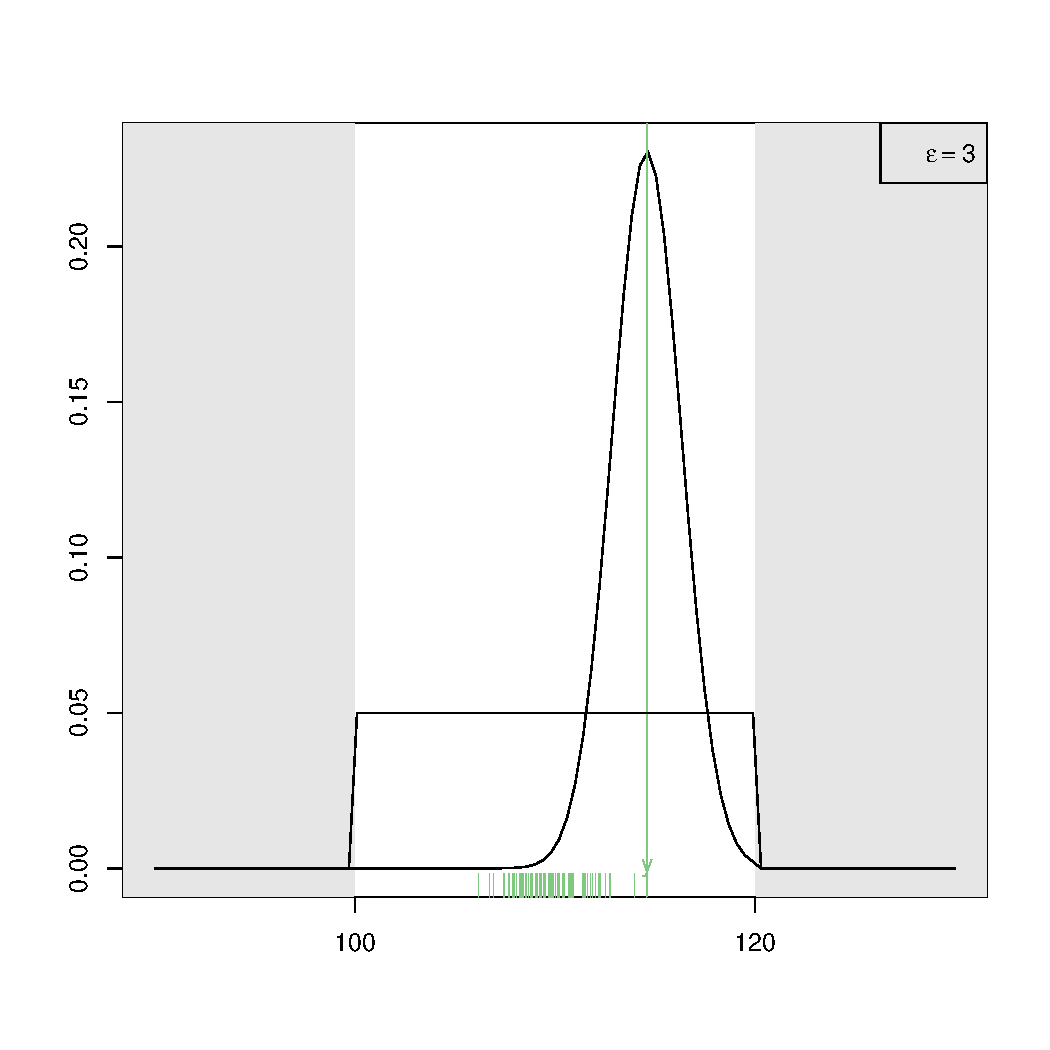
\includegraphics[scale=.35]{./Images/concentrate_0.pdf}}%
\only<2>{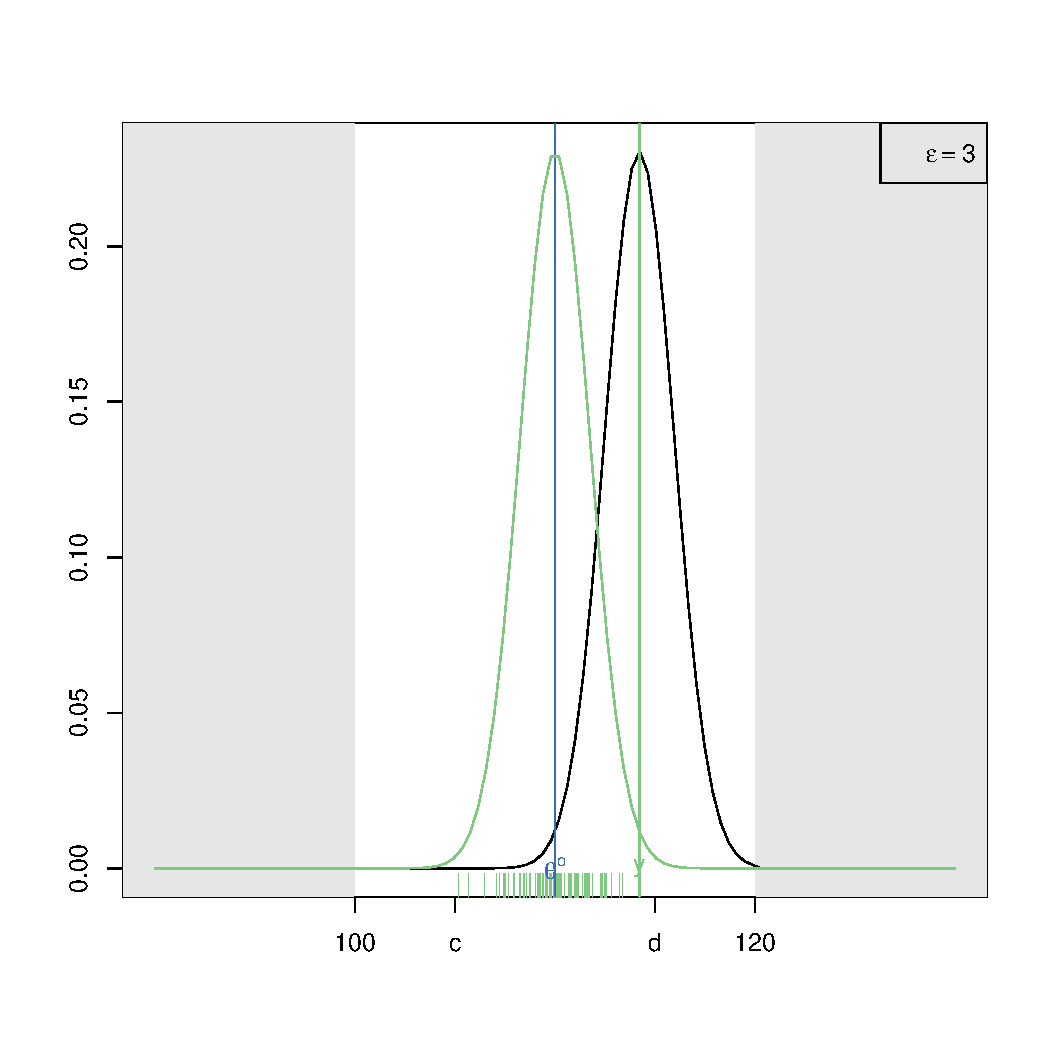
\includegraphics[scale=.35]{./Images/concentrate_1.pdf}}%
\only<3>{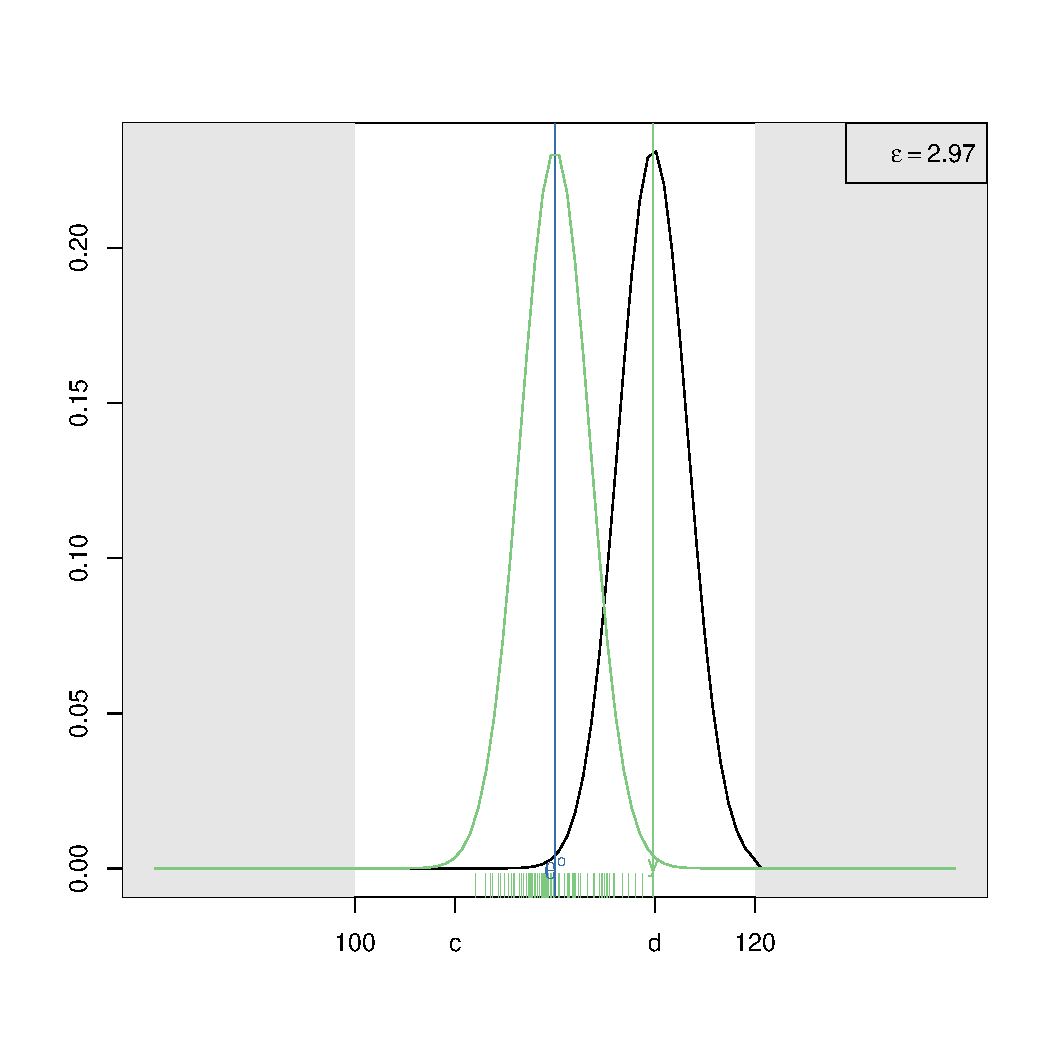
\includegraphics[scale=.35]{./Images/concentrate_2.pdf}}%
\only<4>{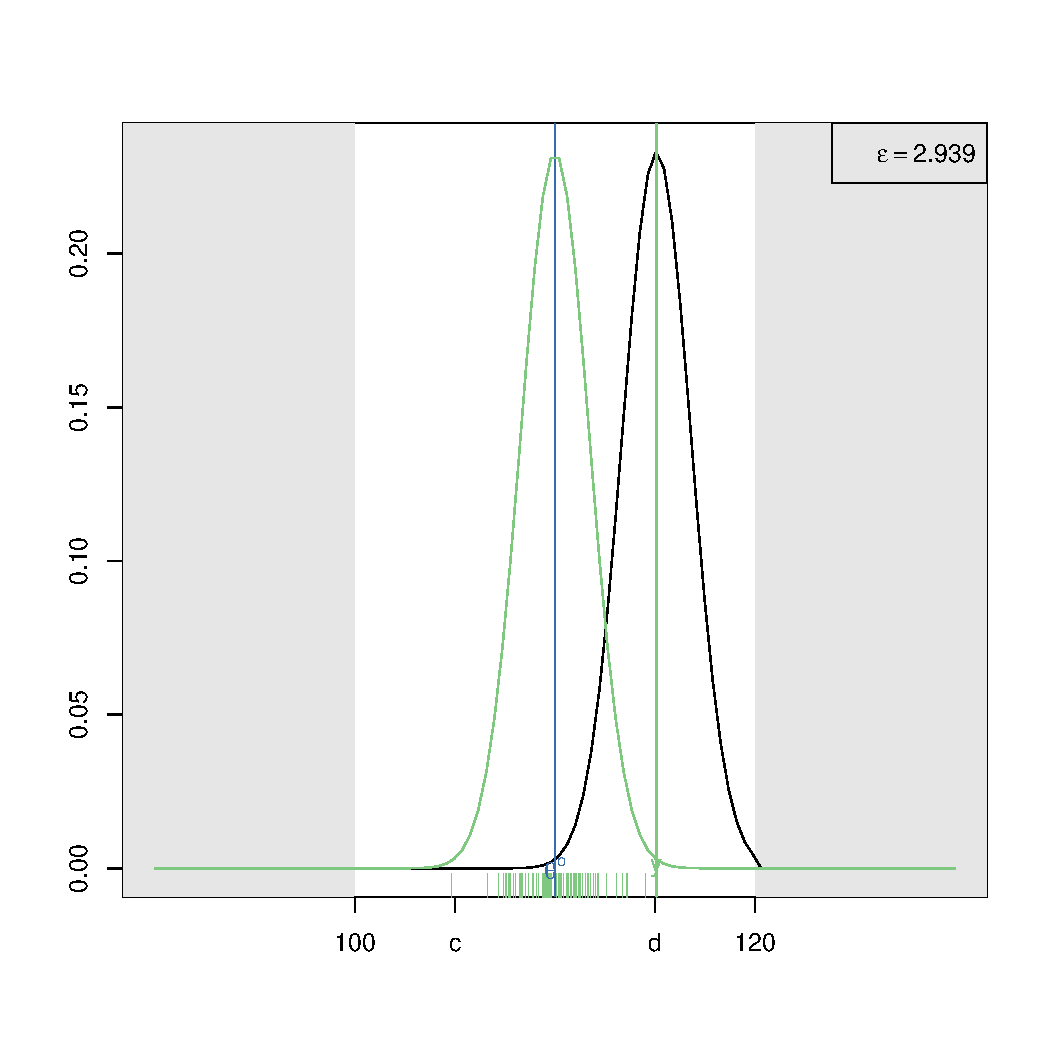
\includegraphics[scale=.35]{./Images/concentrate_3.pdf}}%
\only<5>{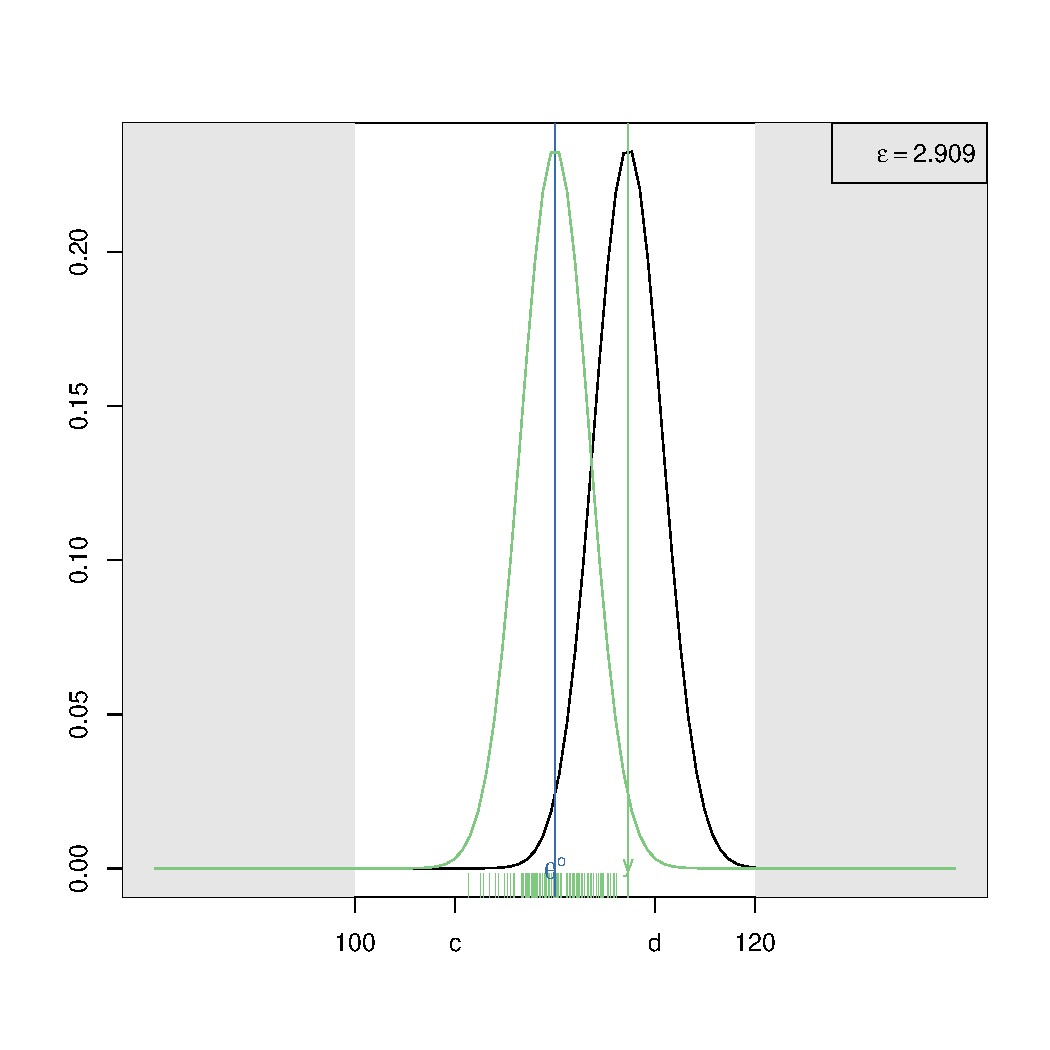
\includegraphics[scale=.35]{./Images/concentrate_4.pdf}}%
\only<6>{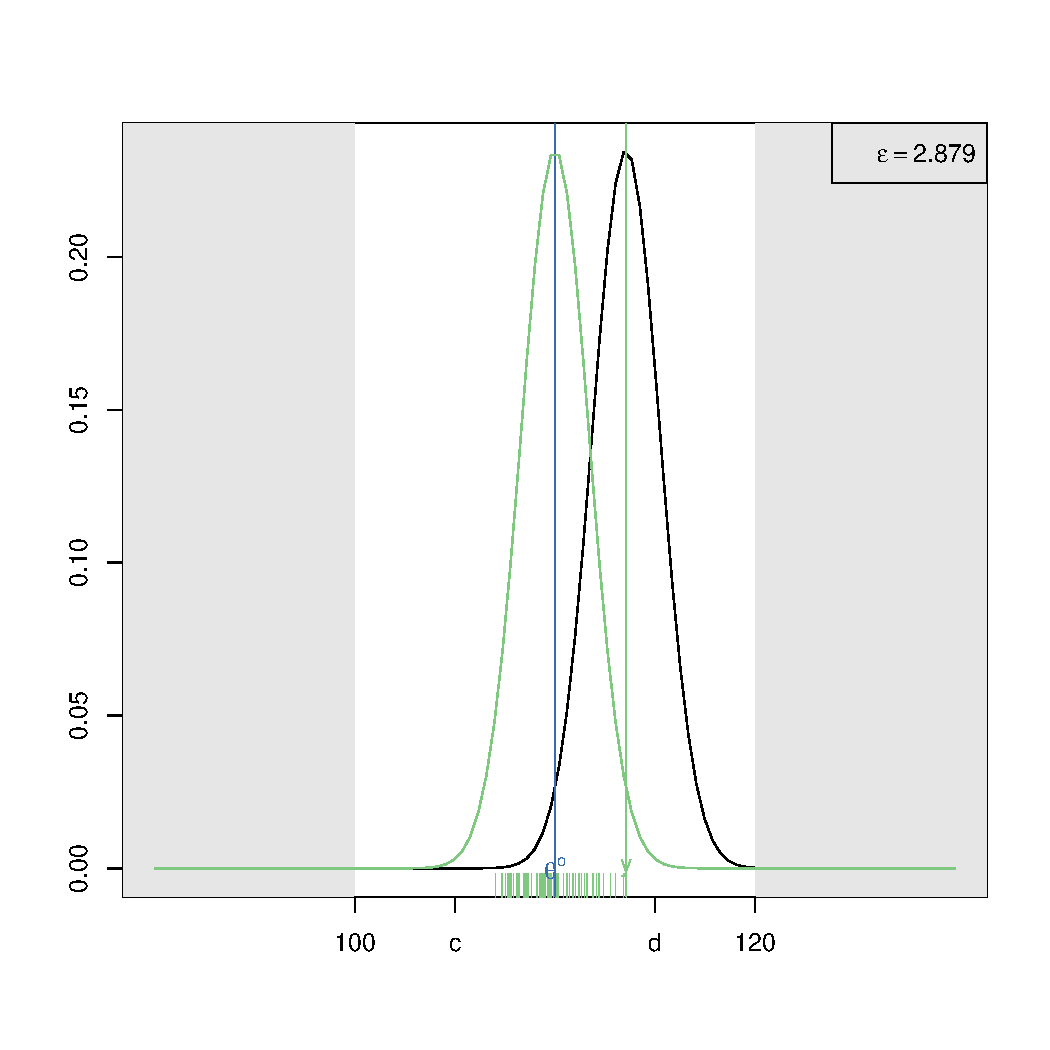
\includegraphics[scale=.35]{./Images/concentrate_5.pdf}}%
\only<7>{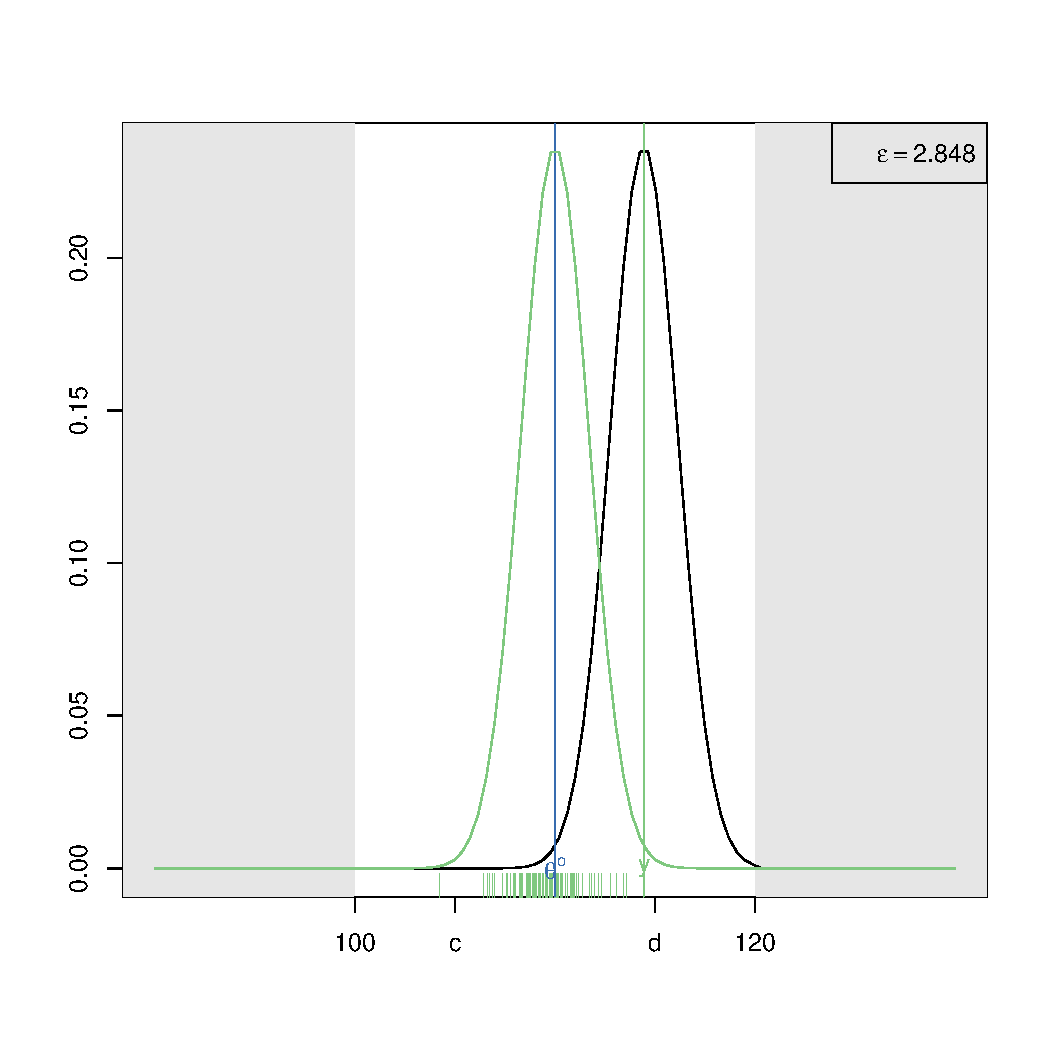
\includegraphics[scale=.35]{./Images/concentrate_6.pdf}}%
\only<8>{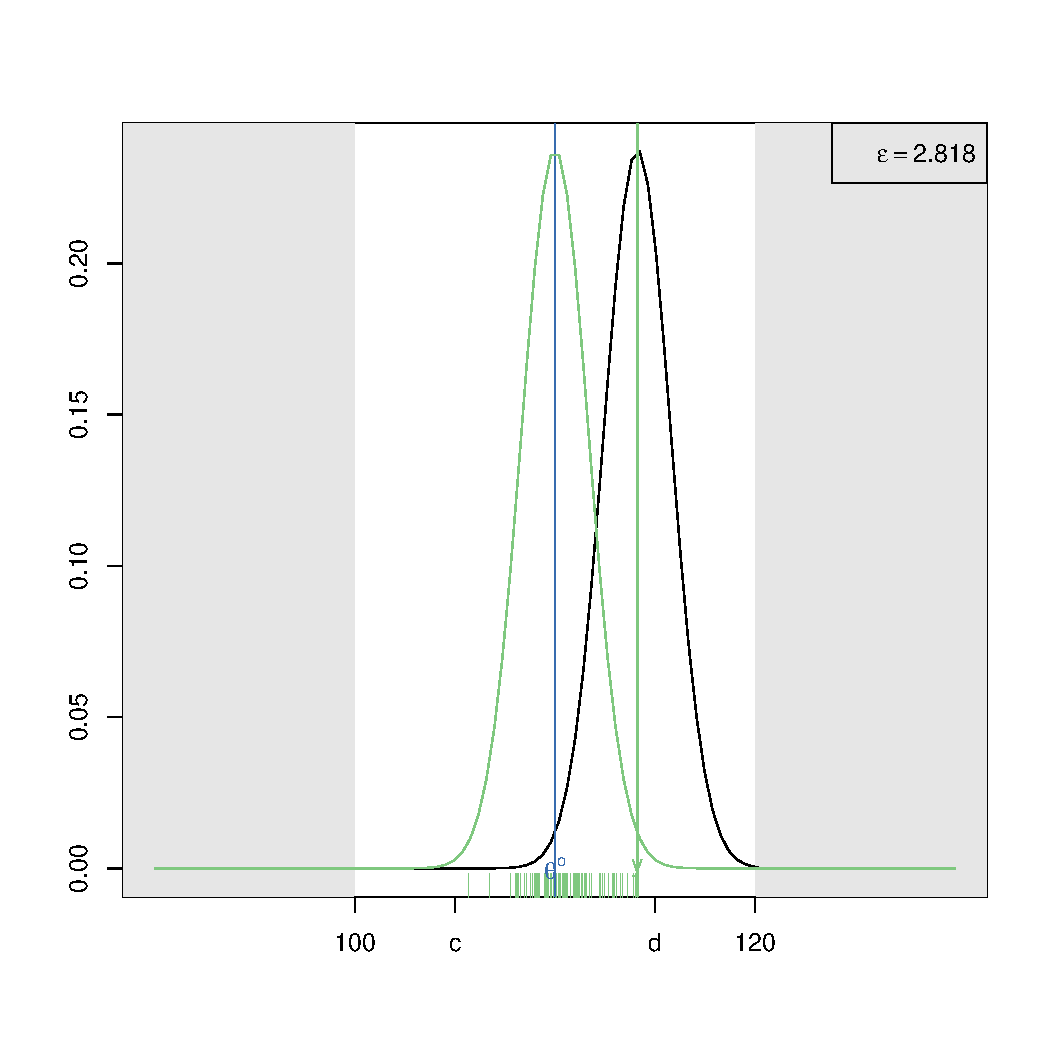
\includegraphics[scale=.35]{./Images/concentrate_7.pdf}}%
\only<9>{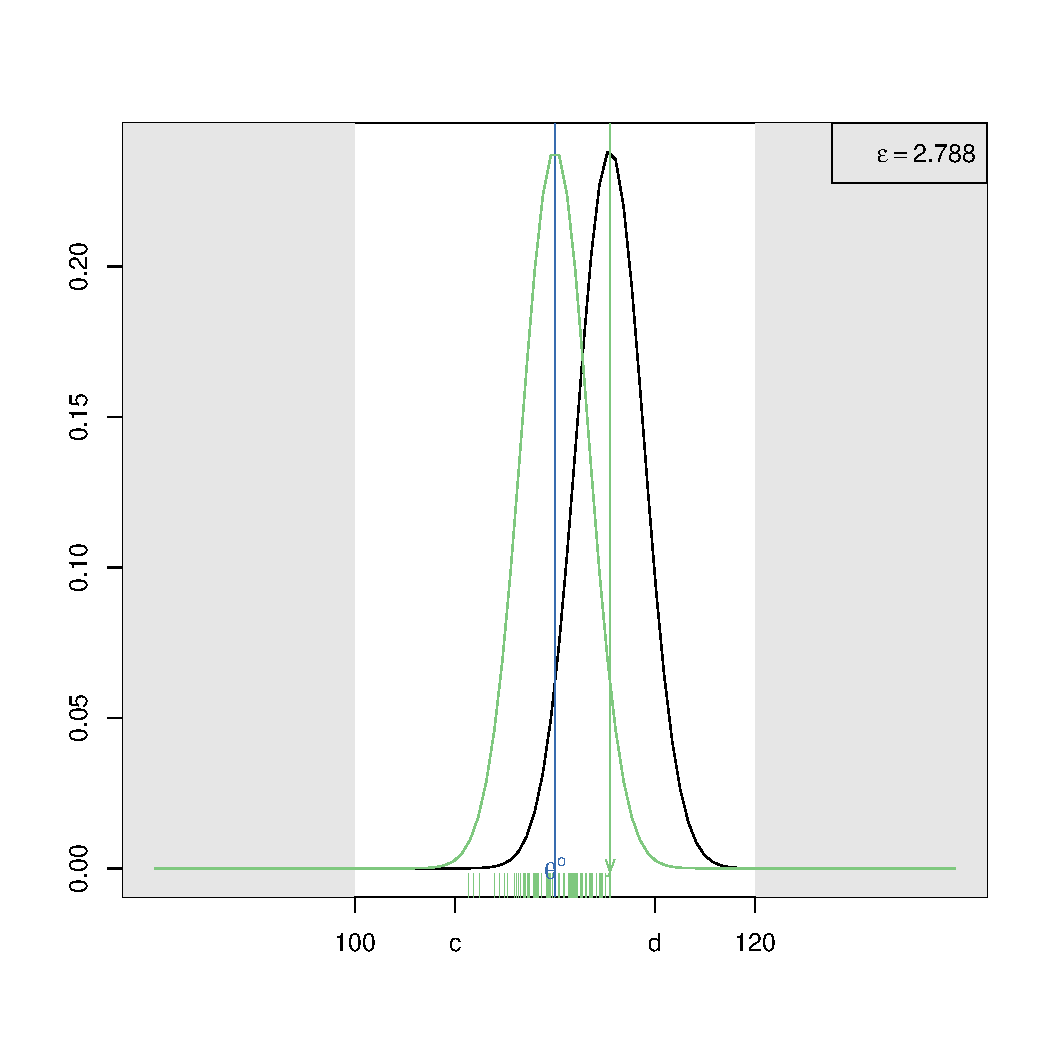
\includegraphics[scale=.35]{./Images/concentrate_8.pdf}}%
\only<10>{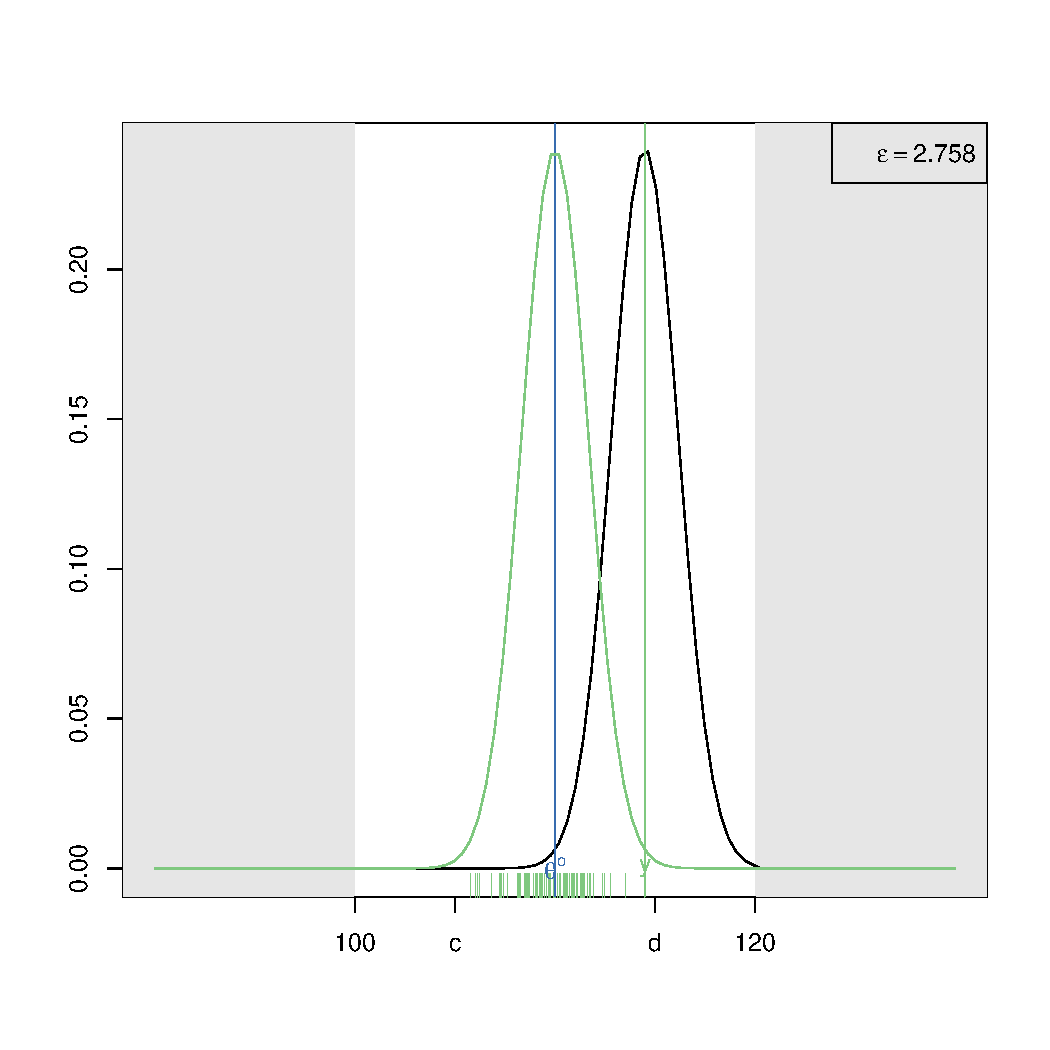
\includegraphics[scale=.35]{./Images/concentrate_9.pdf}}%
\only<11>{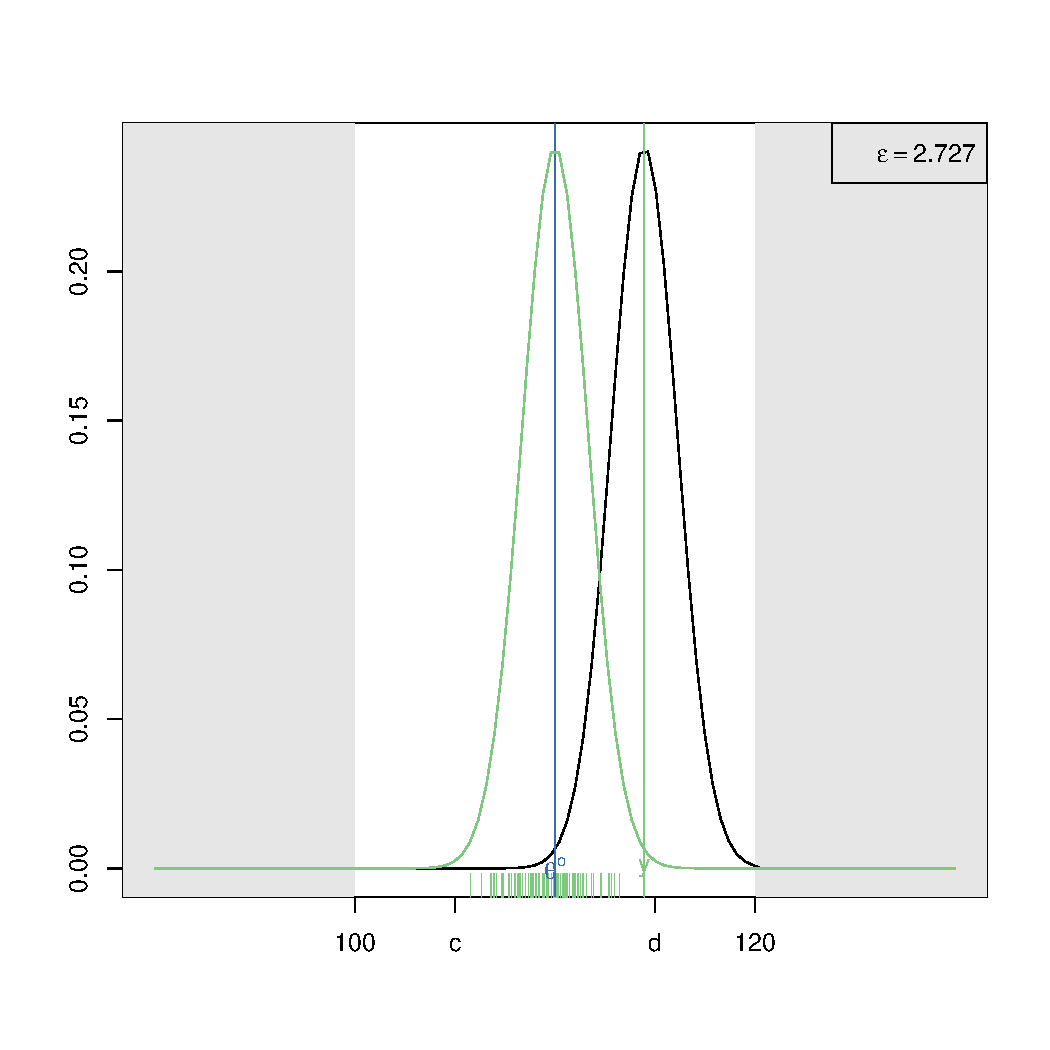
\includegraphics[scale=.35]{./Images/concentrate_10.pdf}}%
\only<12>{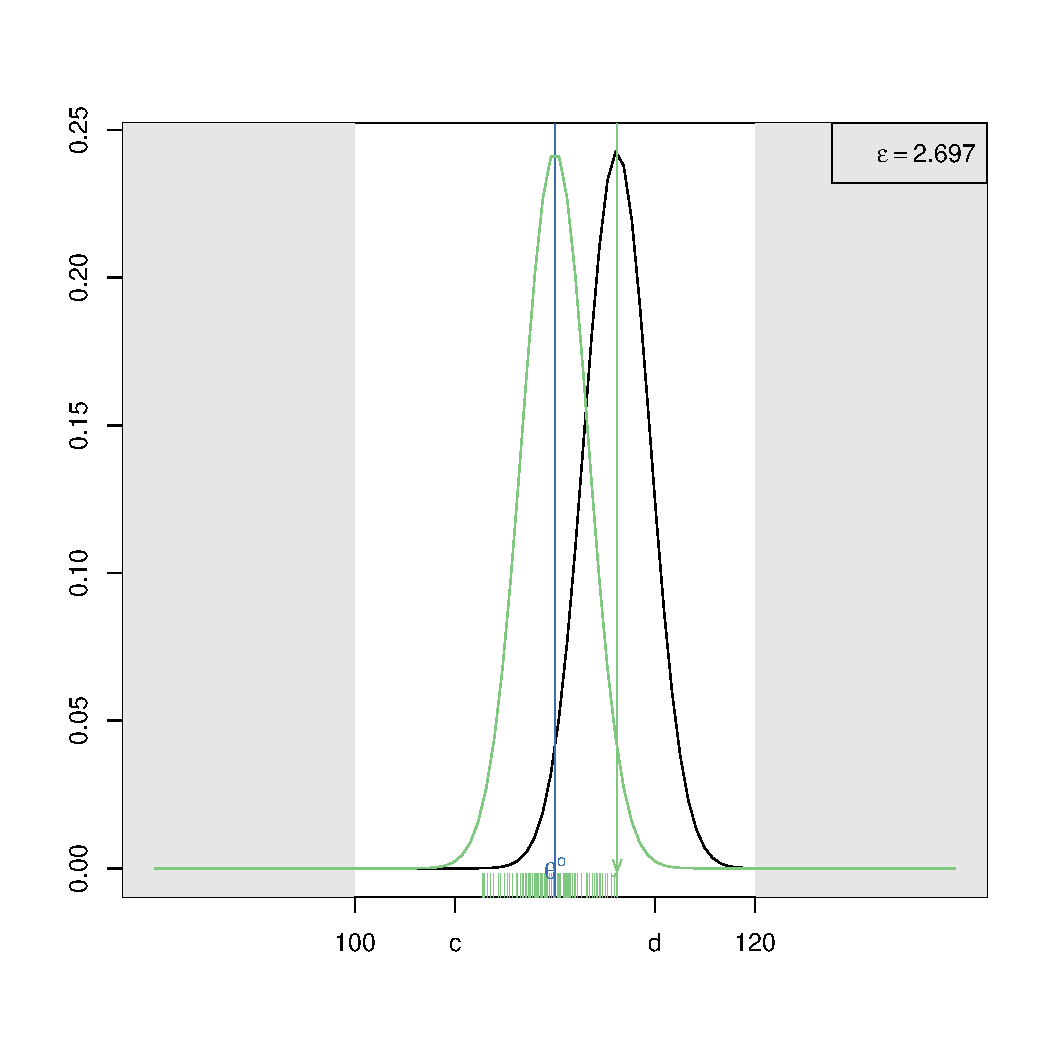
\includegraphics[scale=.35]{./Images/concentrate_11.pdf}}%
\only<13>{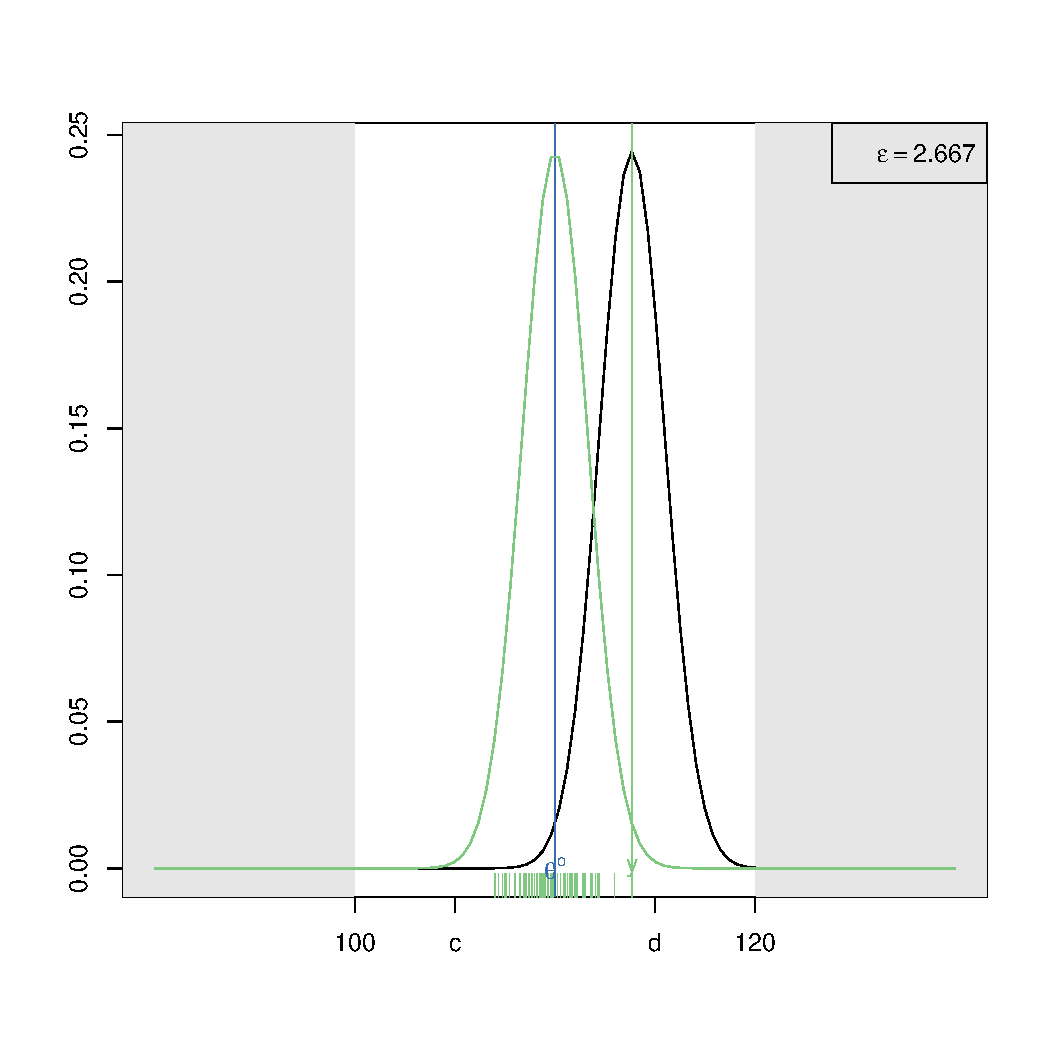
\includegraphics[scale=.35]{./Images/concentrate_12.pdf}}%
\only<14>{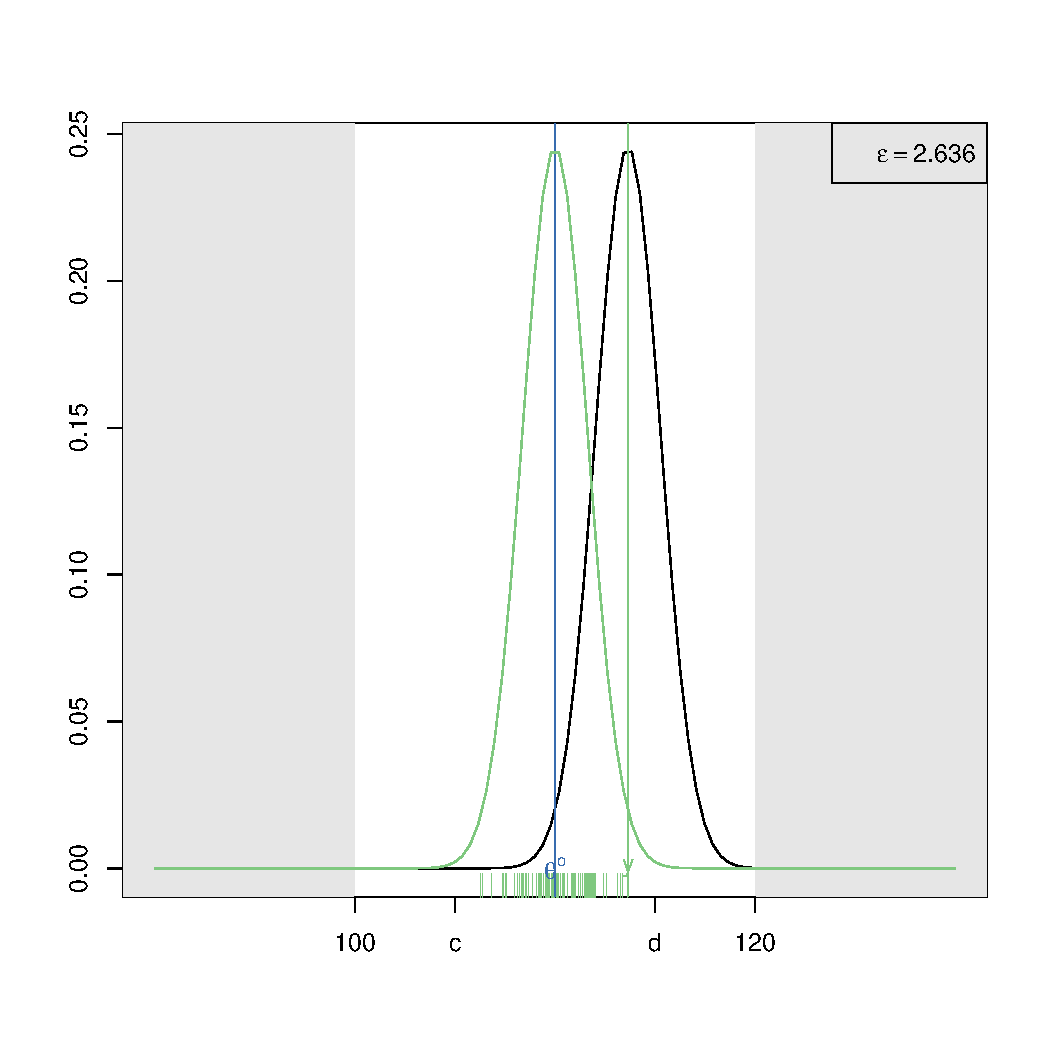
\includegraphics[scale=.35]{./Images/concentrate_13.pdf}}%
\only<15>{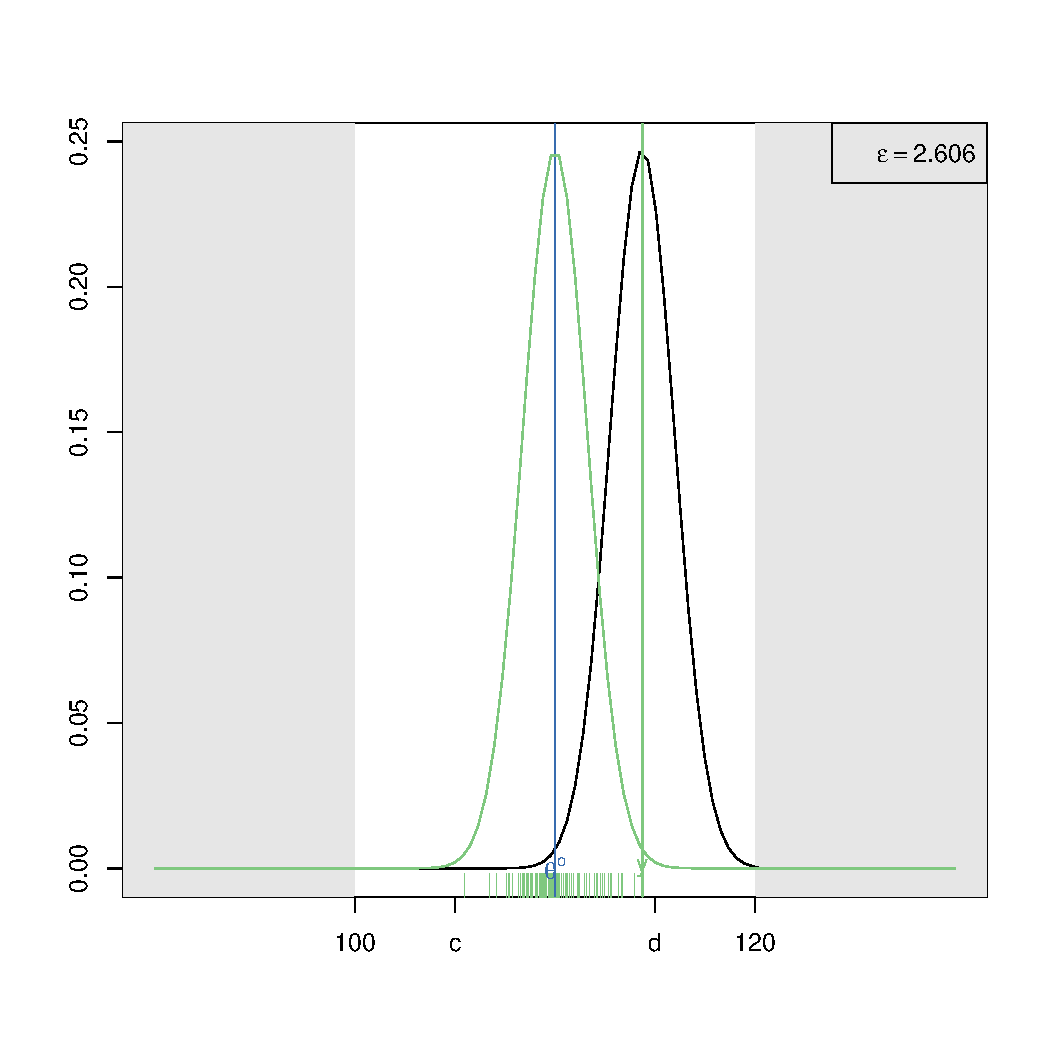
\includegraphics[scale=.35]{./Images/concentrate_14.pdf}}%
\only<16>{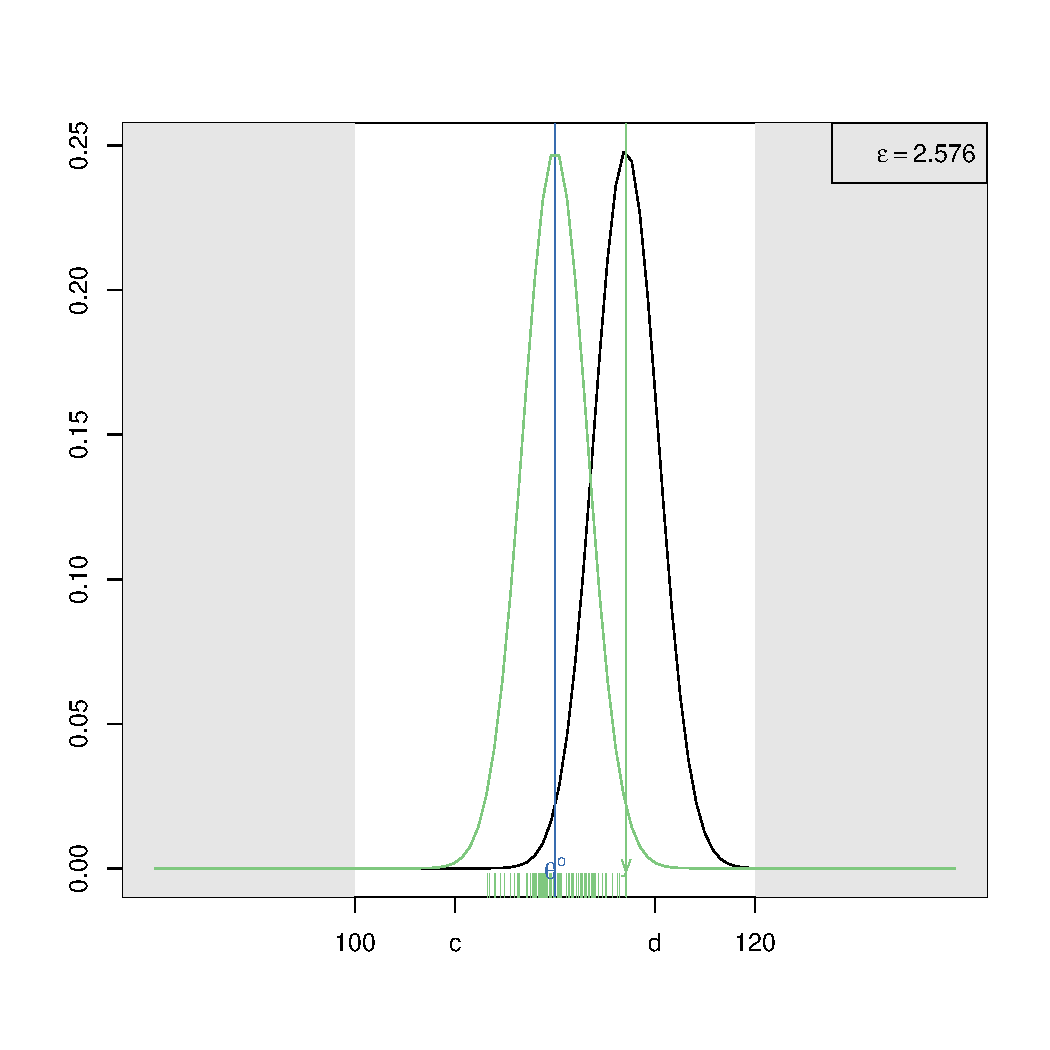
\includegraphics[scale=.35]{./Images/concentrate_15.pdf}}%
\only<17>{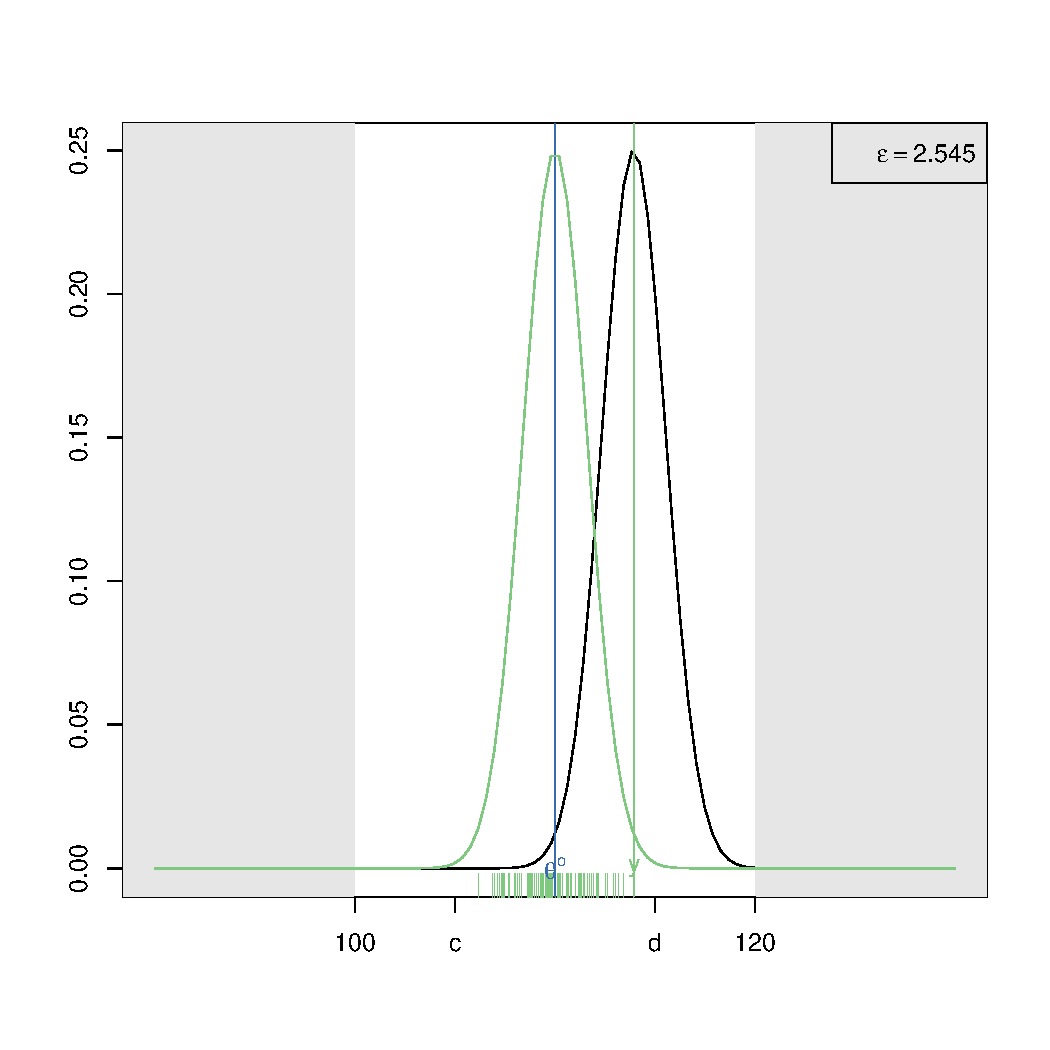
\includegraphics[scale=.35]{./Images/concentrate_16.pdf}}%
\only<18>{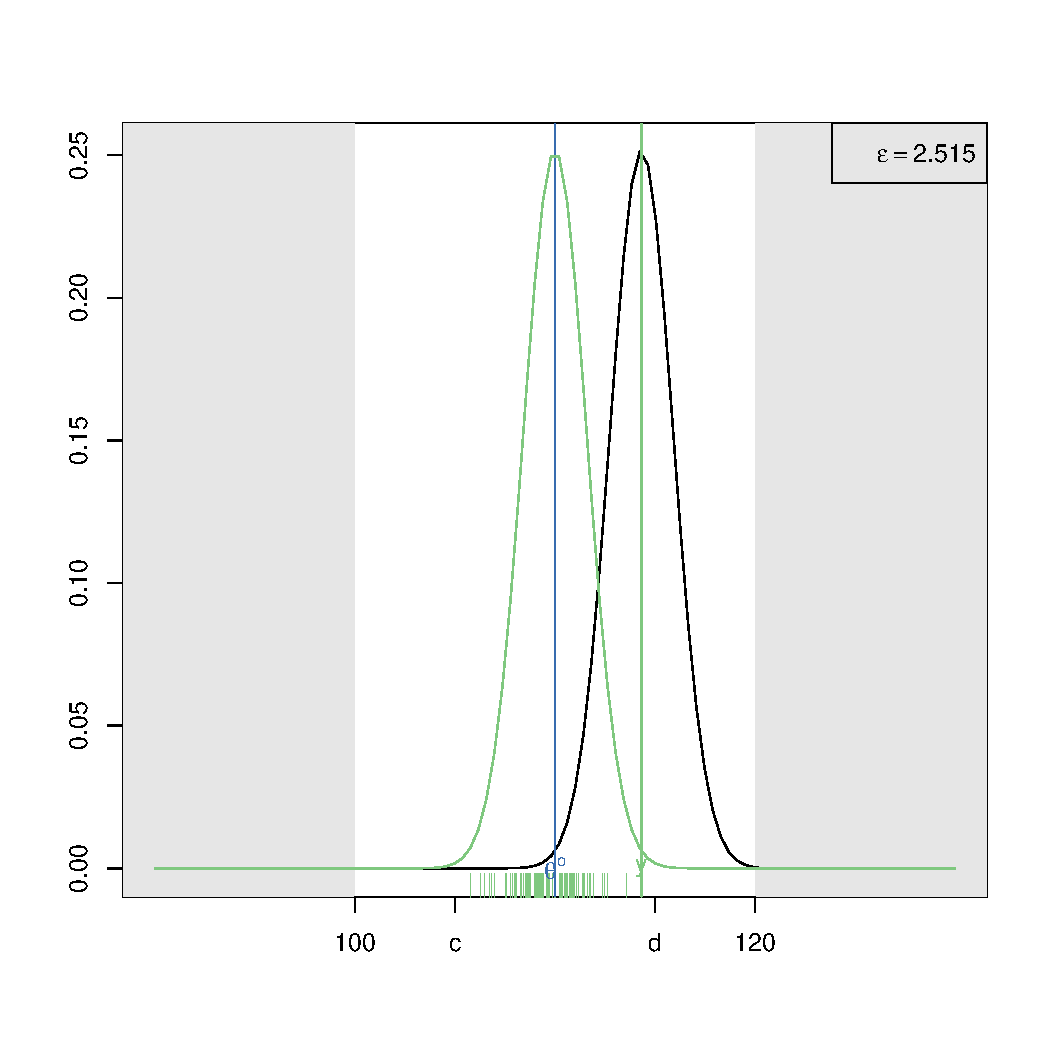
\includegraphics[scale=.35]{./Images/concentrate_17.pdf}}%
\only<19>{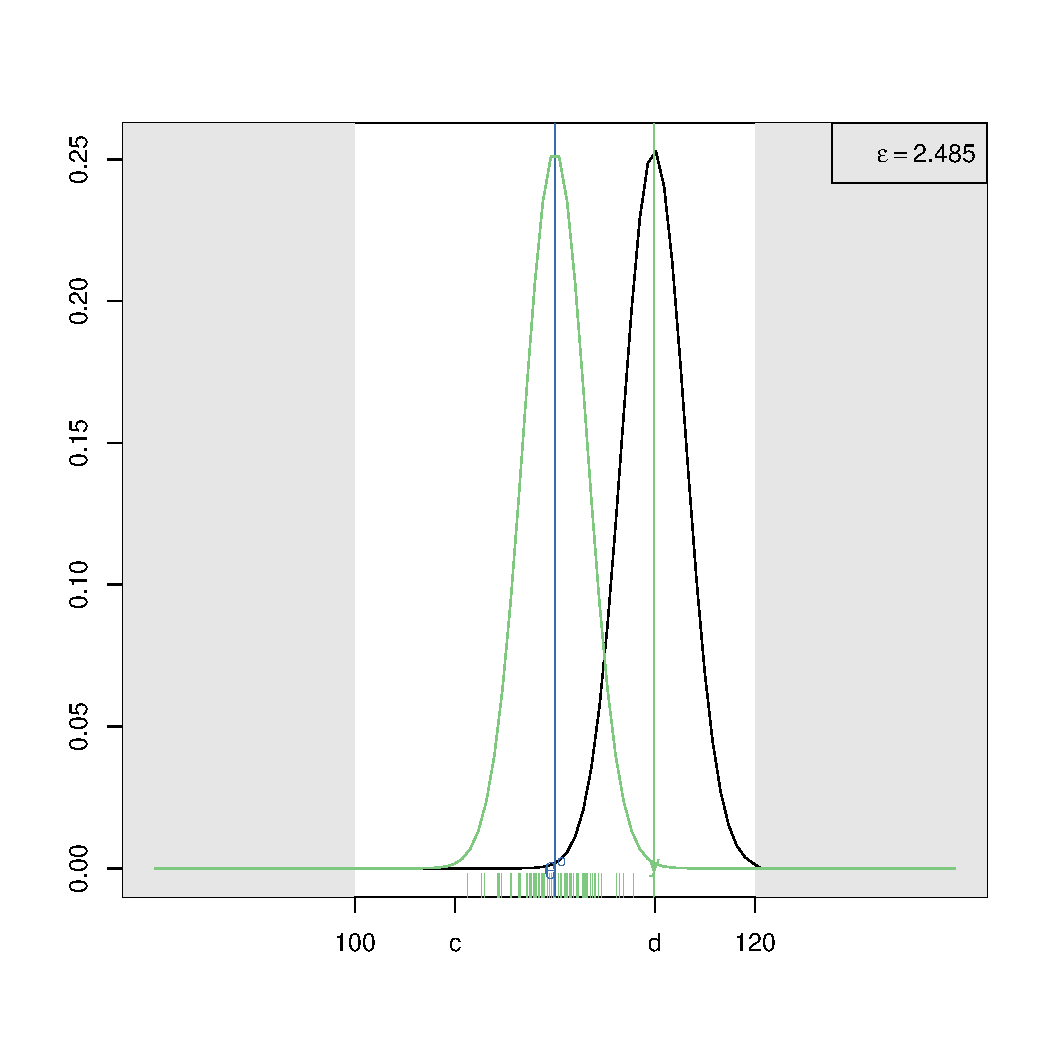
\includegraphics[scale=.35]{./Images/concentrate_18.pdf}}%
\only<20>{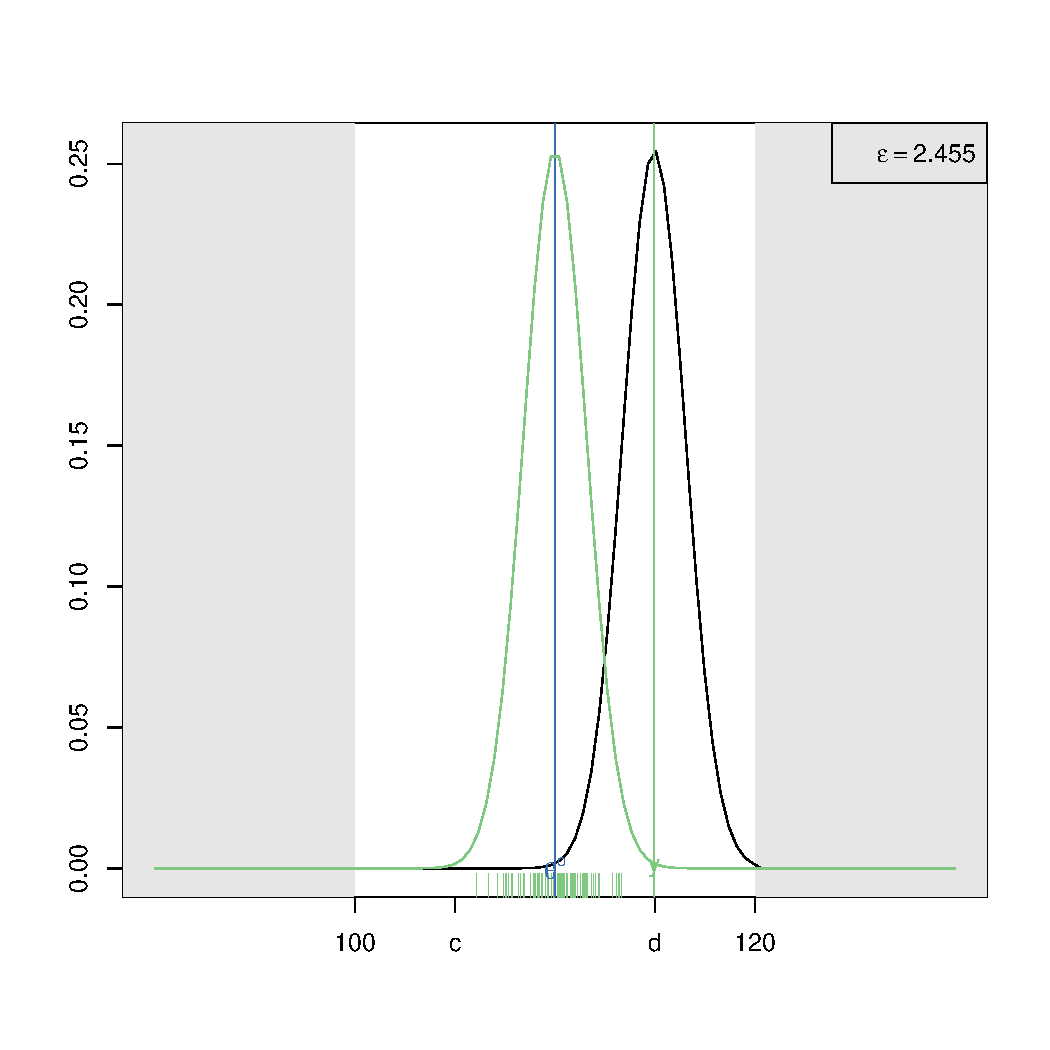
\includegraphics[scale=.35]{./Images/concentrate_19.pdf}}%
\only<21>{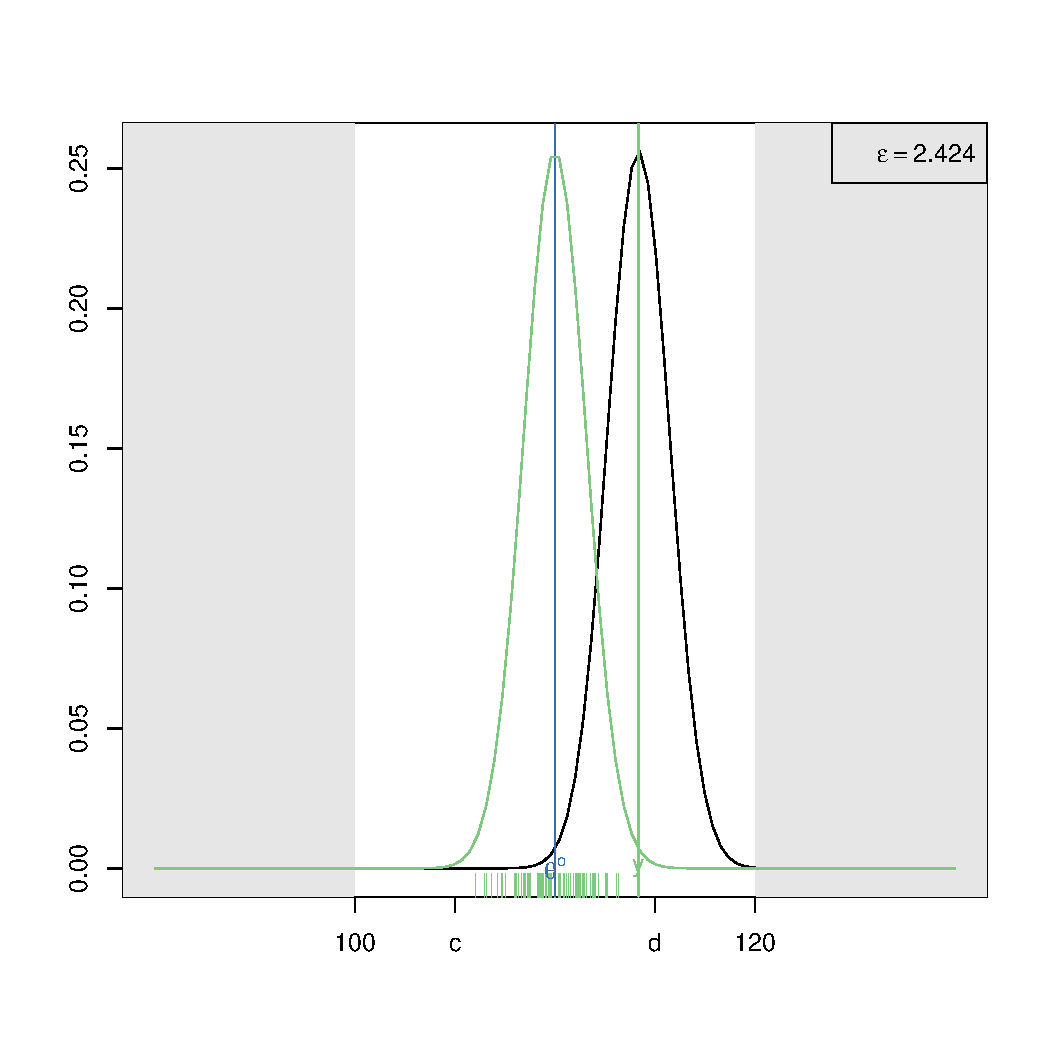
\includegraphics[scale=.35]{./Images/concentrate_20.pdf}}%
\only<22>{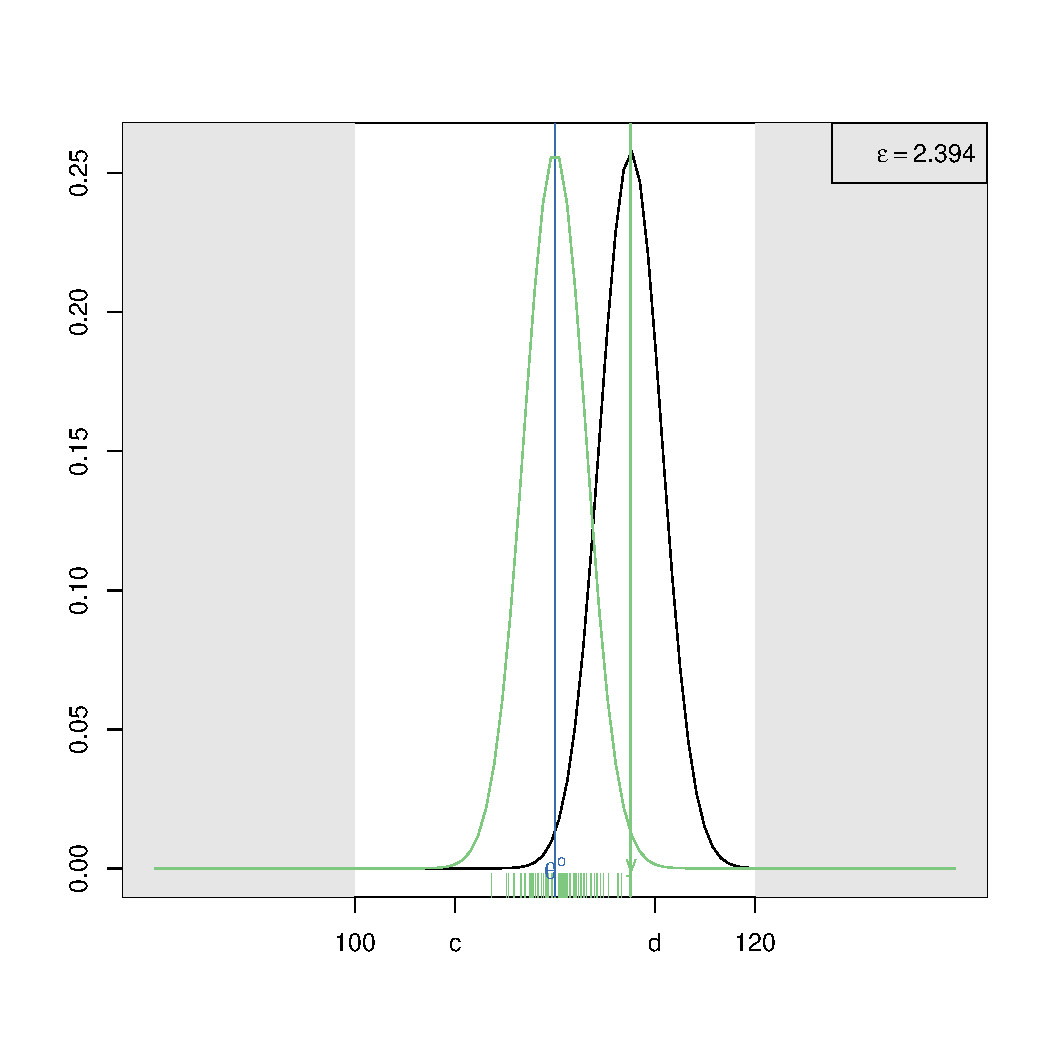
\includegraphics[scale=.35]{./Images/concentrate_21.pdf}}%
\only<23>{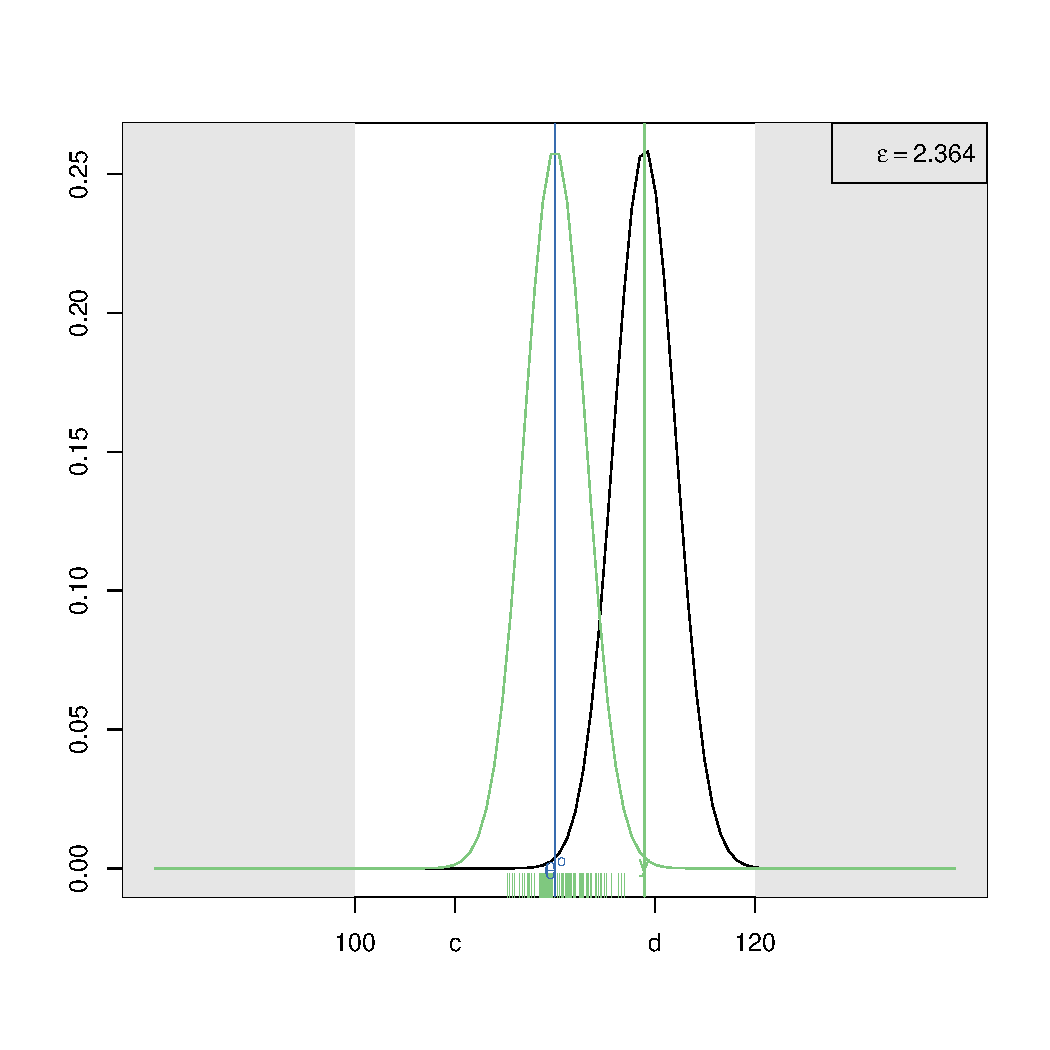
\includegraphics[scale=.35]{./Images/concentrate_22.pdf}}%
\only<24>{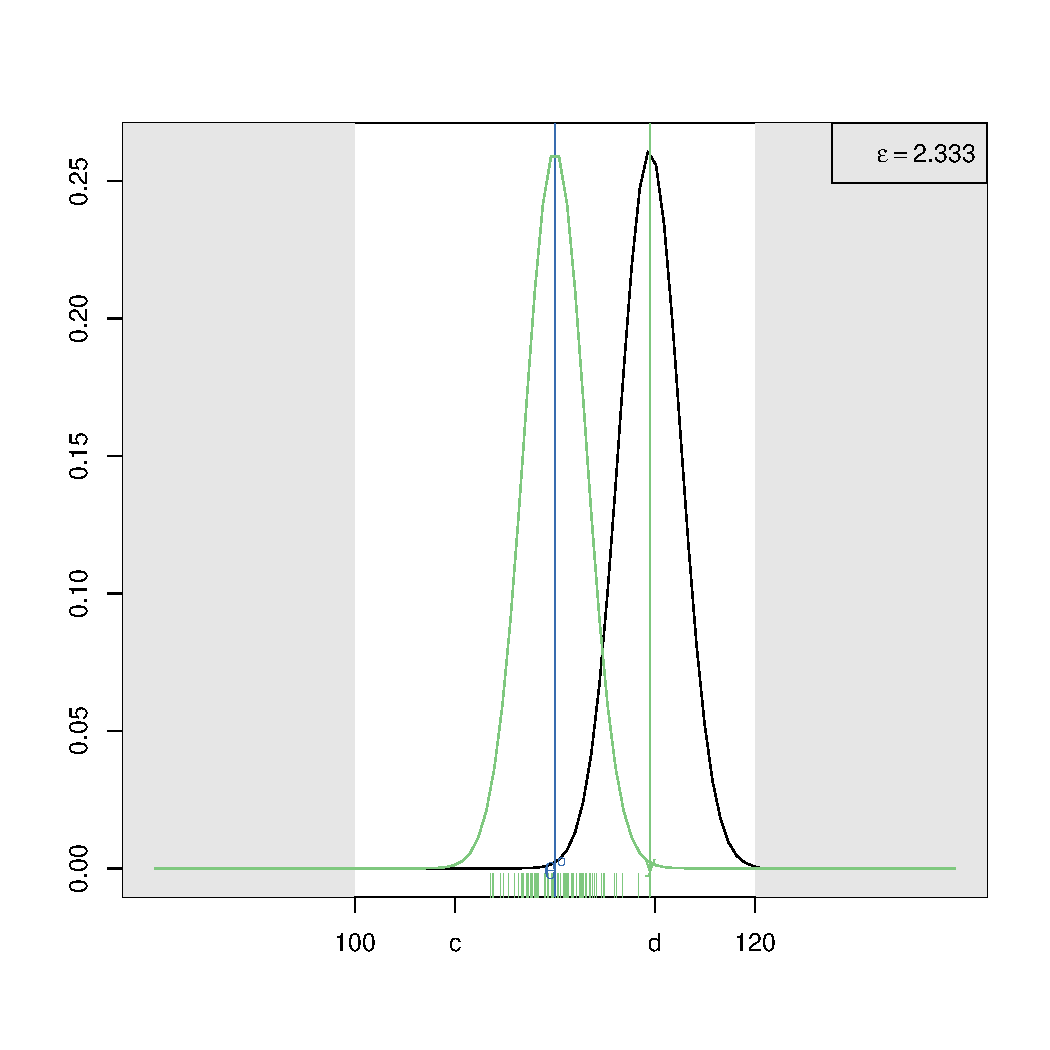
\includegraphics[scale=.35]{./Images/concentrate_23.pdf}}%
\only<25>{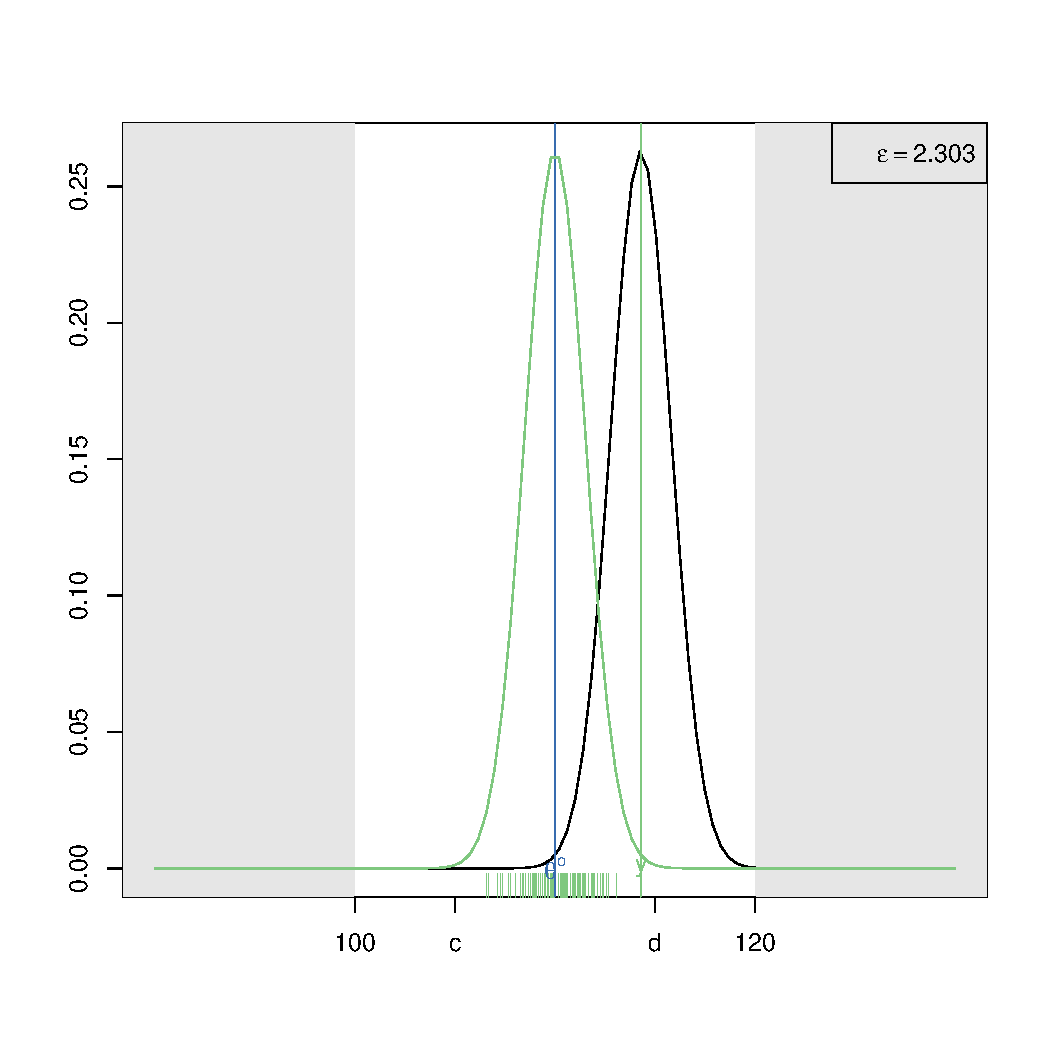
\includegraphics[scale=.35]{./Images/concentrate_24.pdf}}%
\only<26>{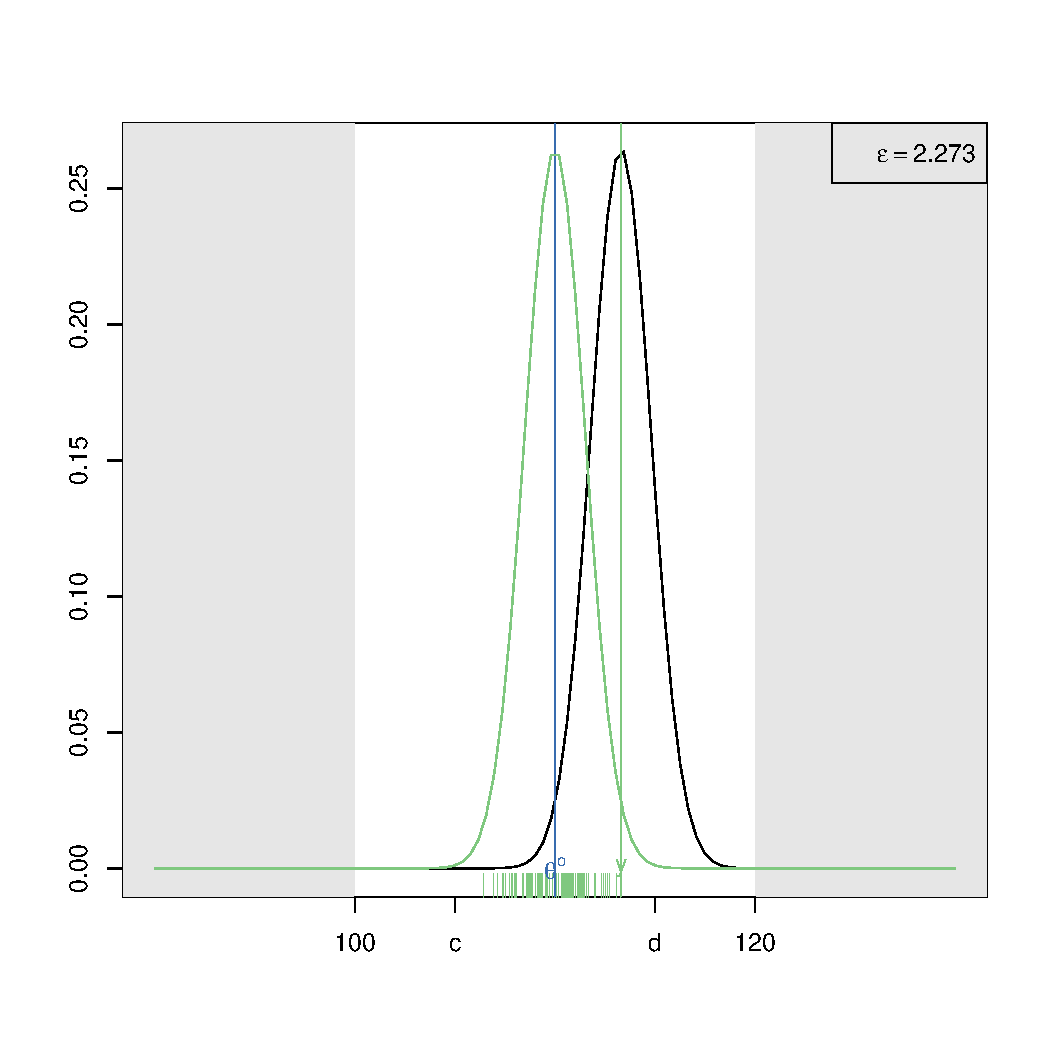
\includegraphics[scale=.35]{./Images/concentrate_25.pdf}}%
\only<27>{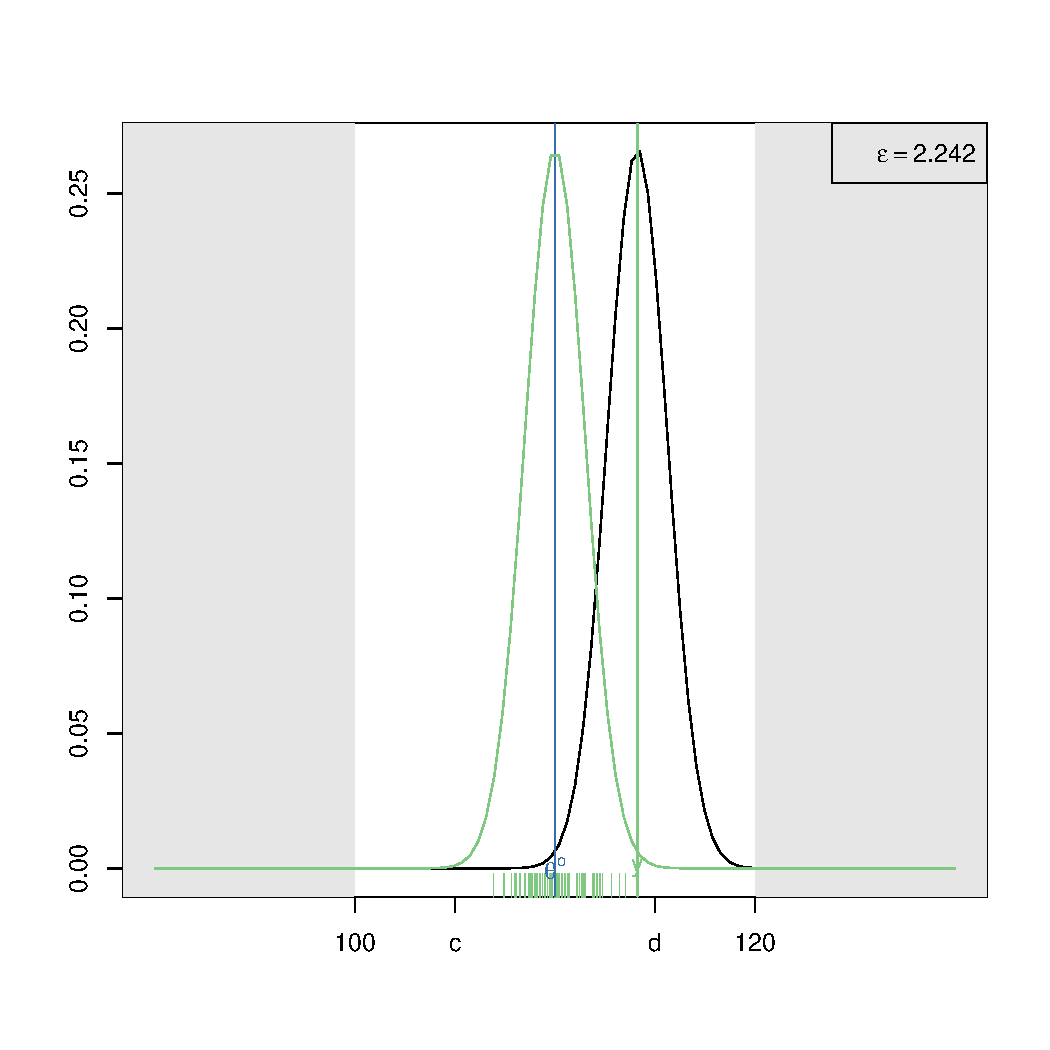
\includegraphics[scale=.35]{./Images/concentrate_26.pdf}}%
\only<28>{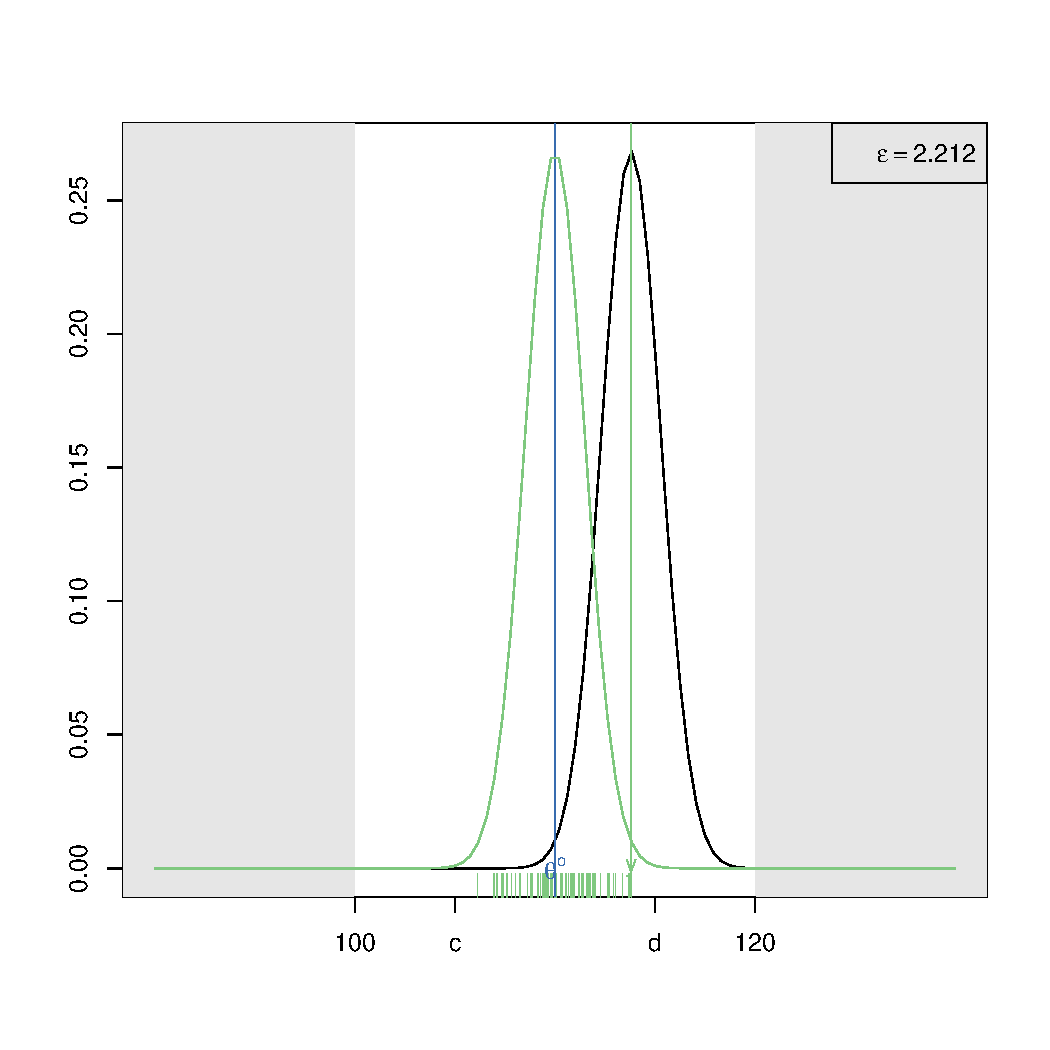
\includegraphics[scale=.35]{./Images/concentrate_27.pdf}}%
\only<29>{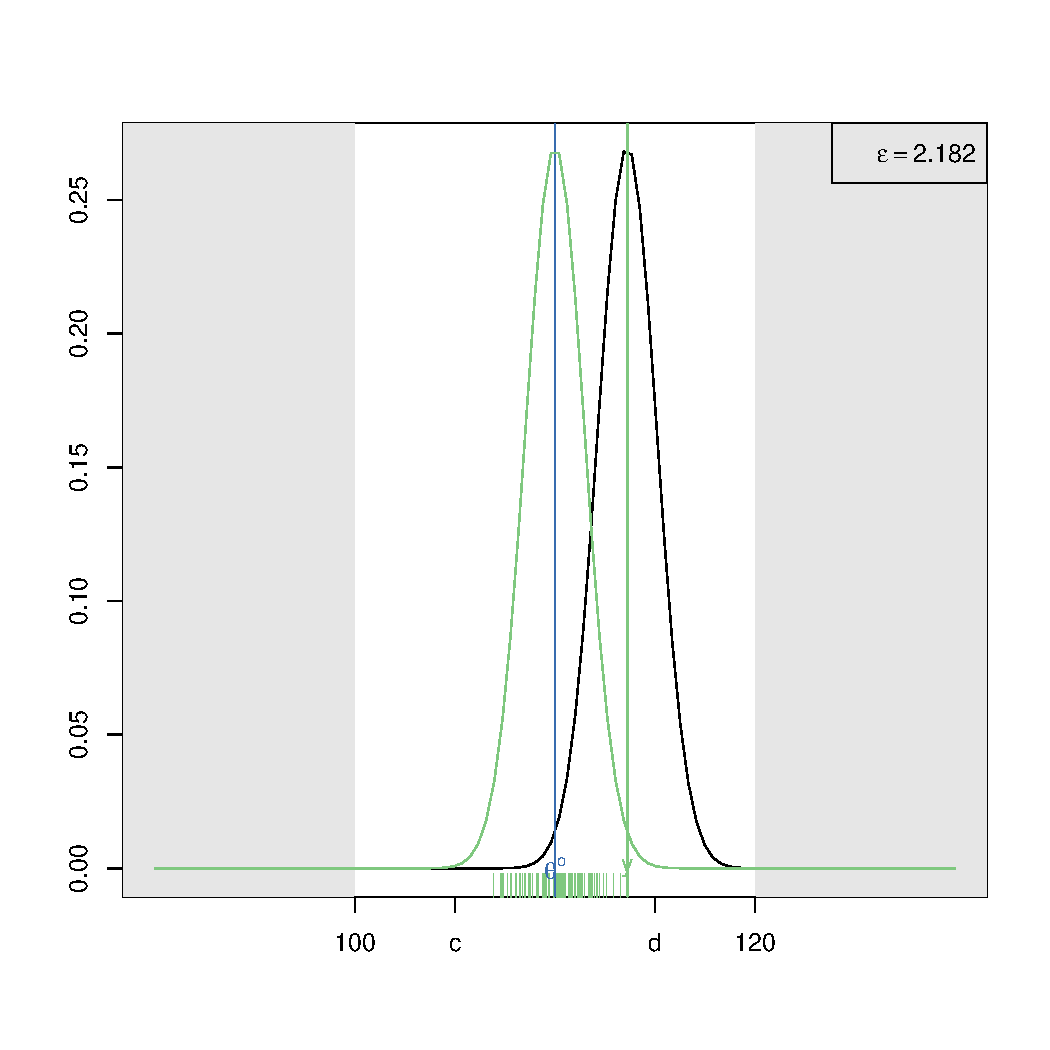
\includegraphics[scale=.35]{./Images/concentrate_28.pdf}}%
\only<30>{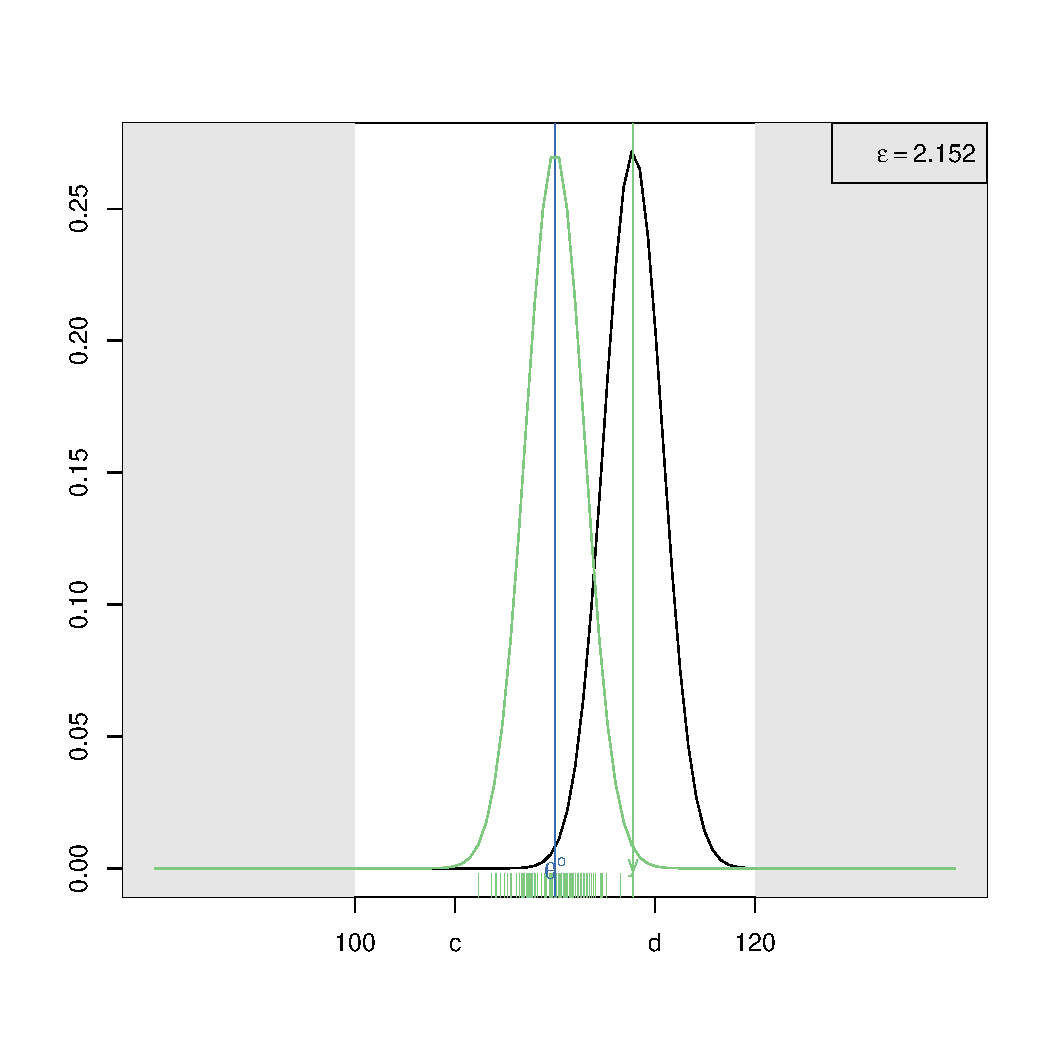
\includegraphics[scale=.35]{./Images/concentrate_29.pdf}}%
\only<31>{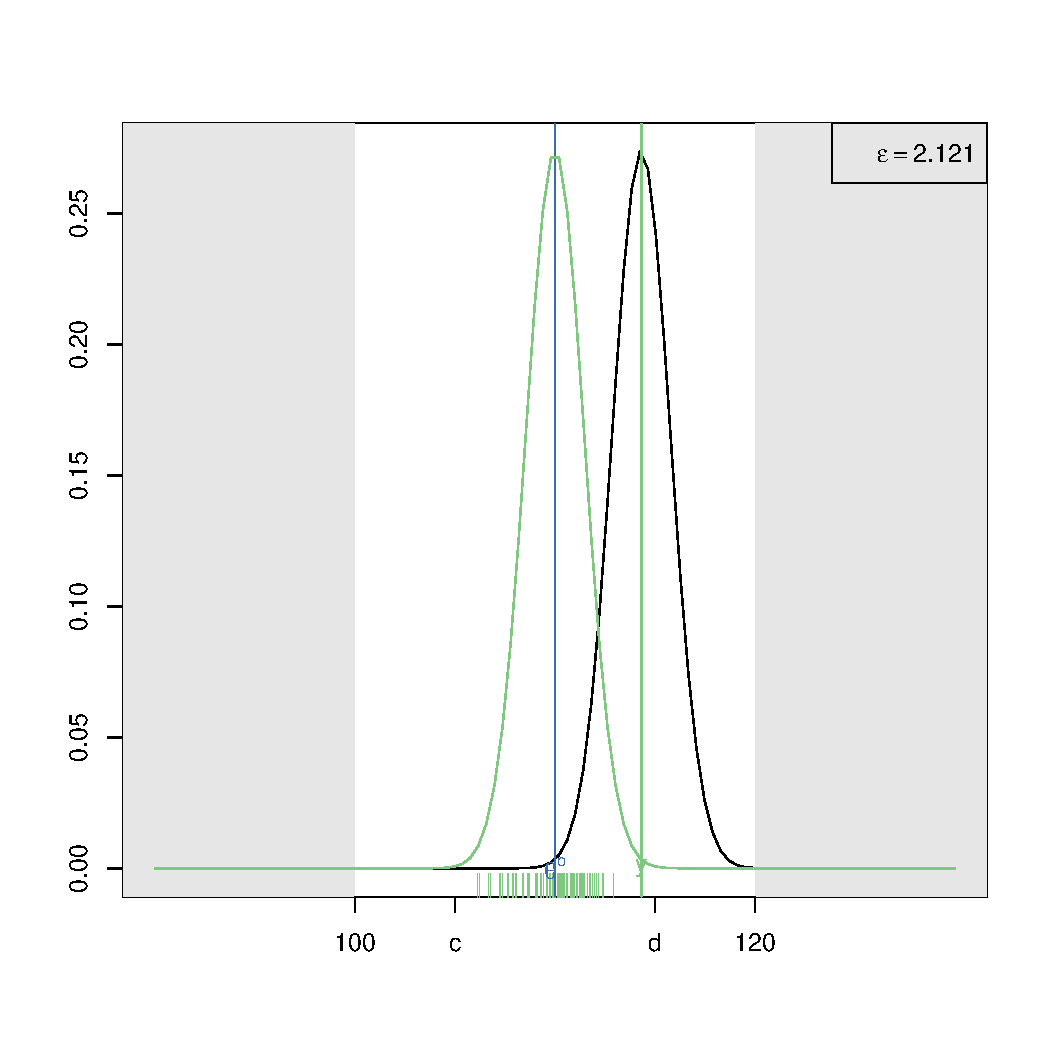
\includegraphics[scale=.35]{./Images/concentrate_30.pdf}}%
\only<32>{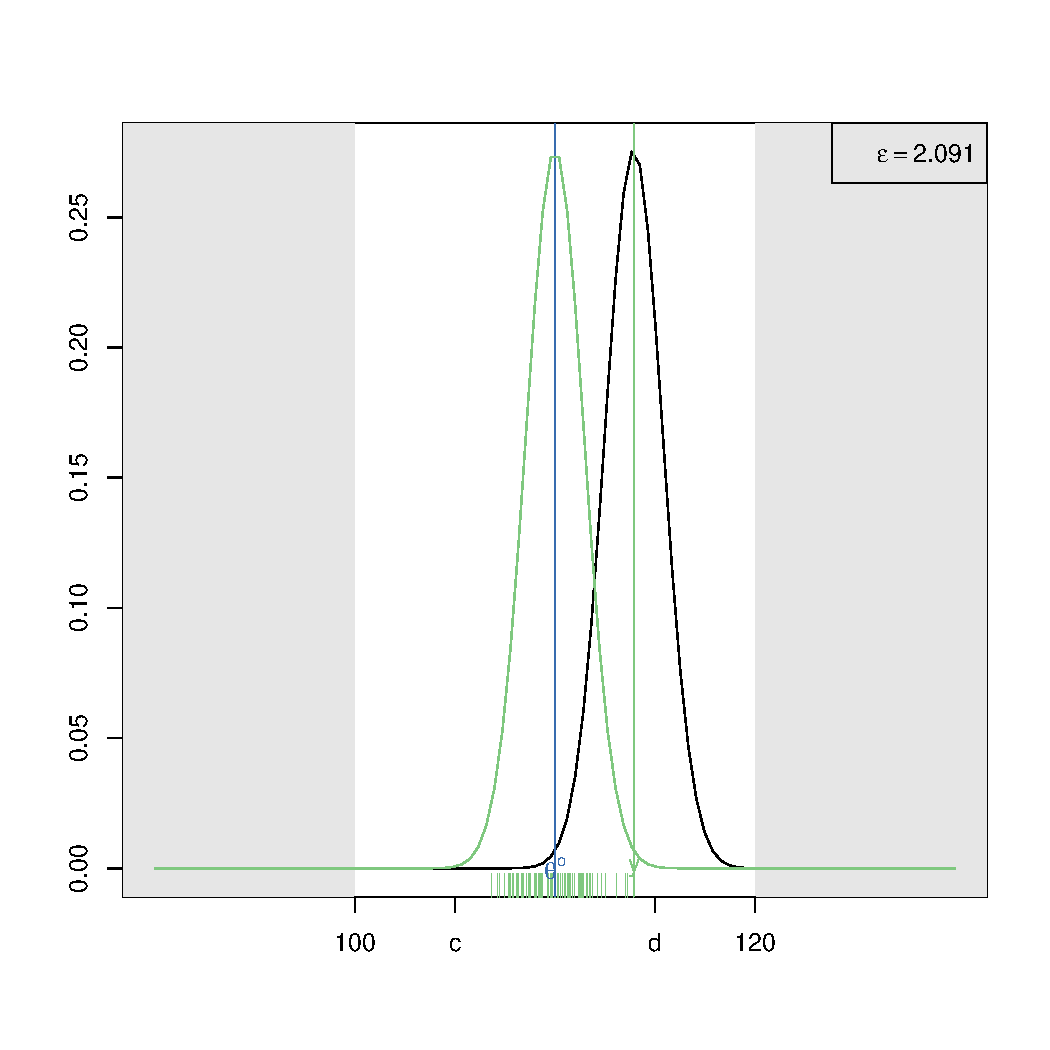
\includegraphics[scale=.35]{./Images/concentrate_31.pdf}}%
\only<33>{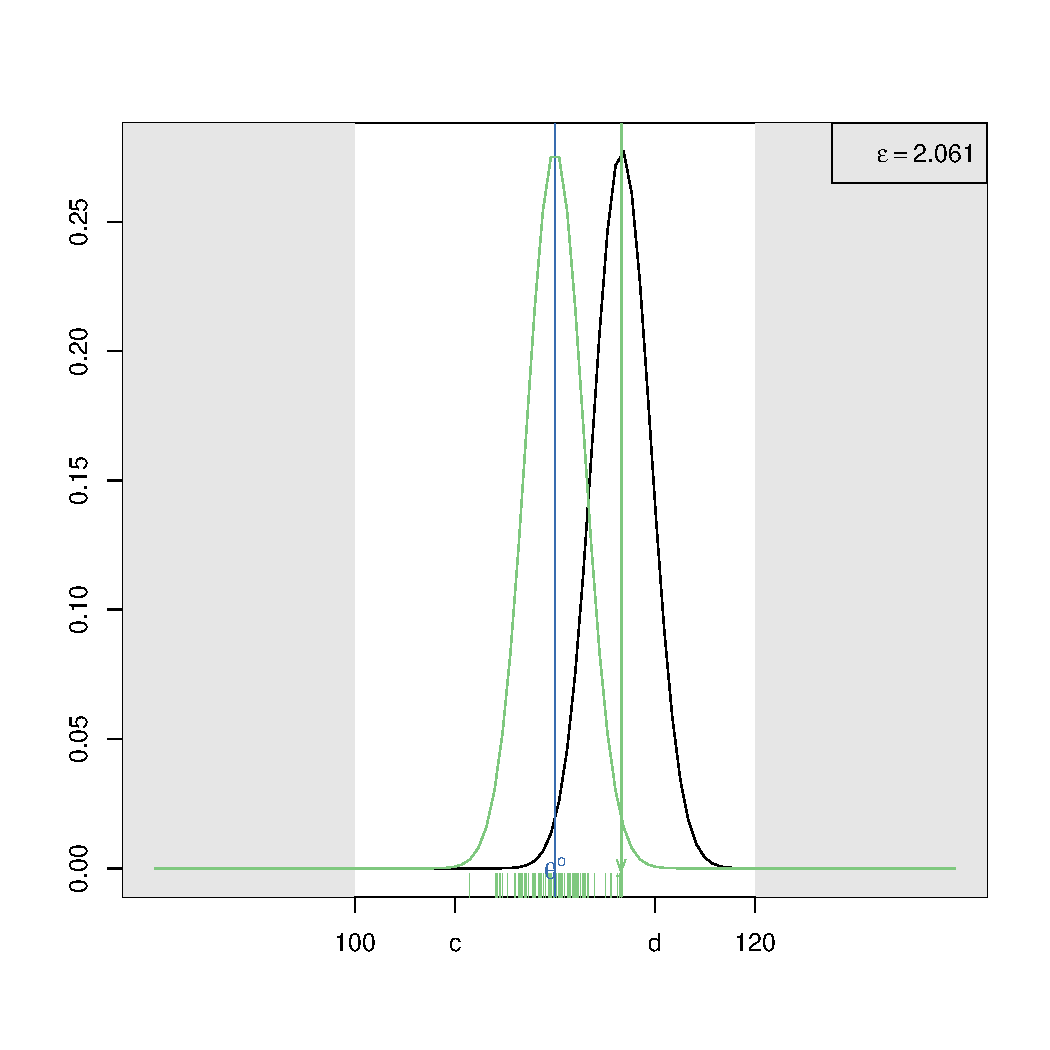
\includegraphics[scale=.35]{./Images/concentrate_32.pdf}}%
\only<34>{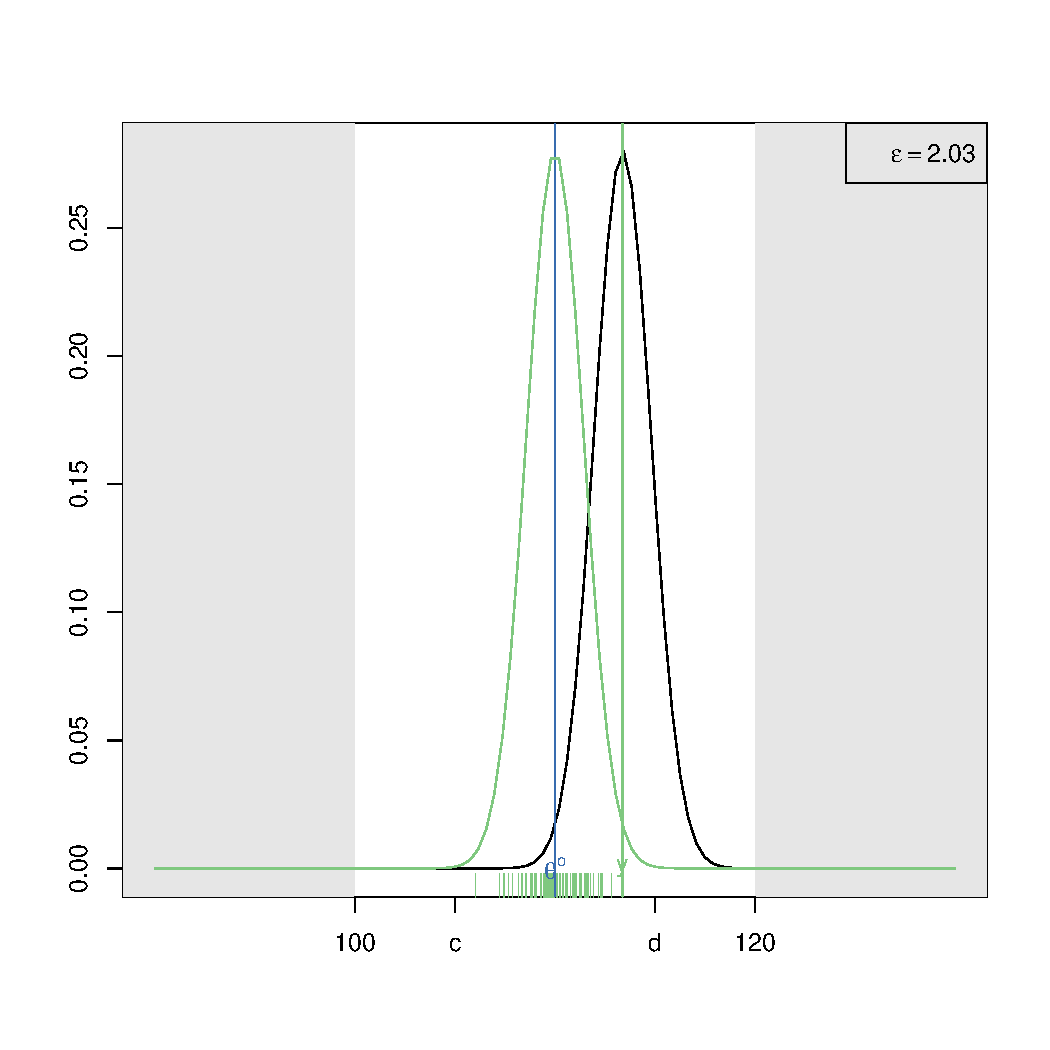
\includegraphics[scale=.35]{./Images/concentrate_33.pdf}}%
\only<35>{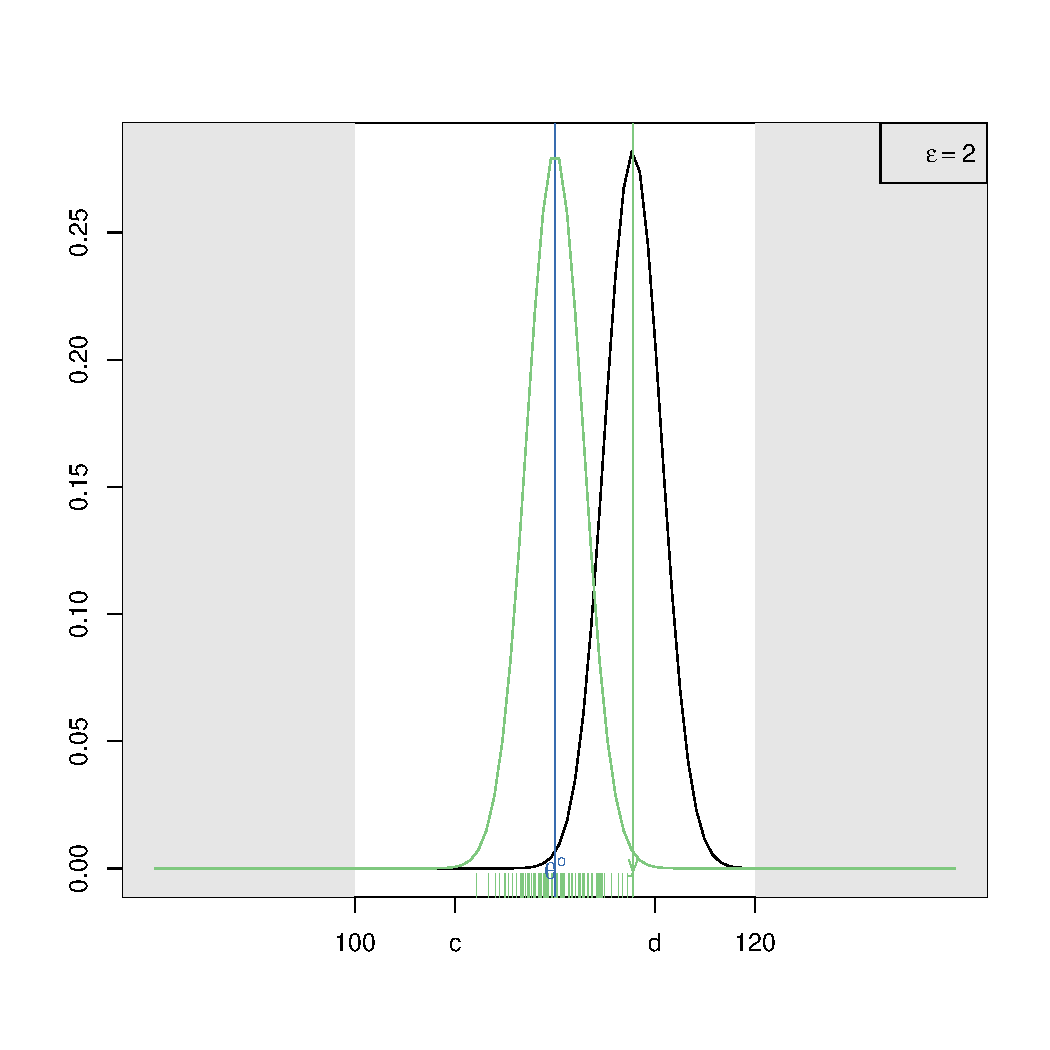
\includegraphics[scale=.35]{./Images/concentrate_34.pdf}}%
\only<36>{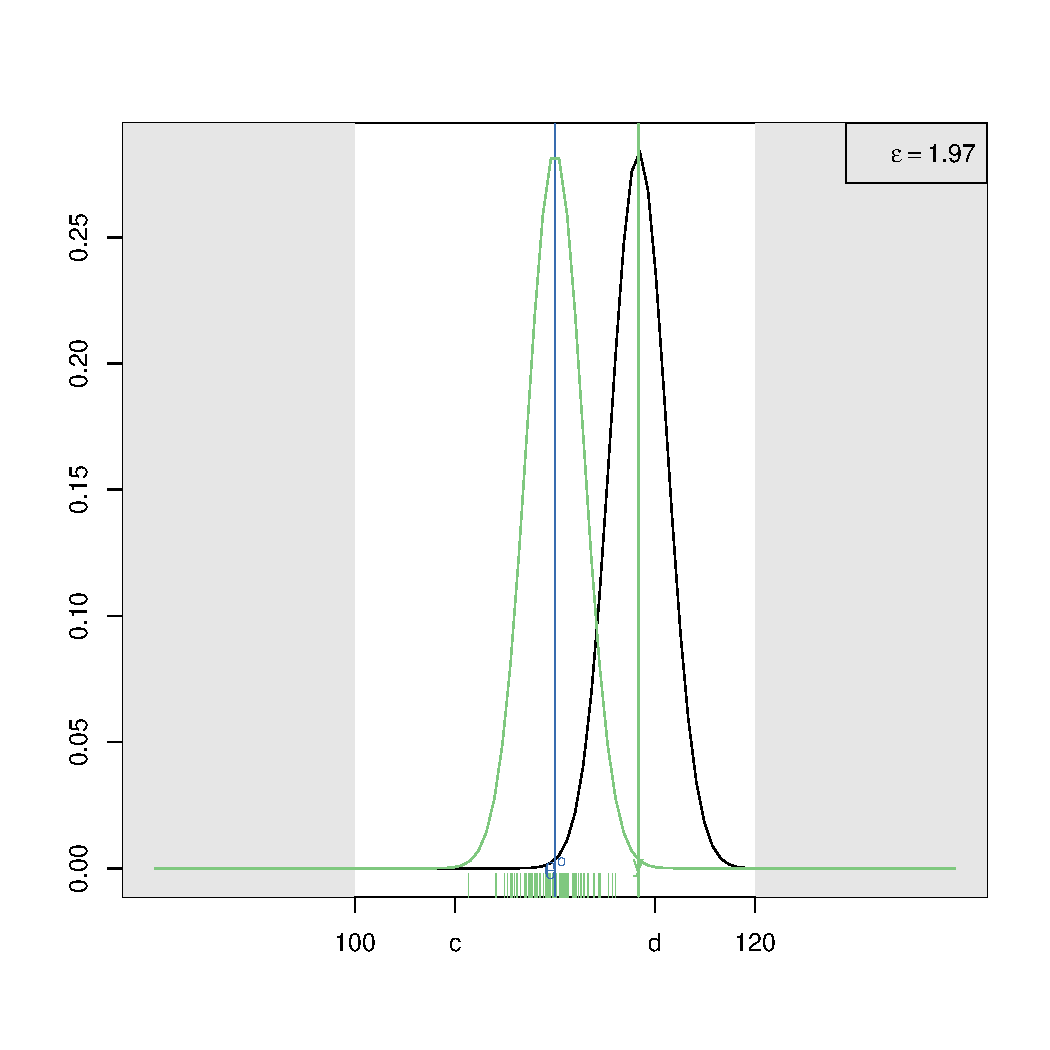
\includegraphics[scale=.35]{./Images/concentrate_35.pdf}}%
\only<37>{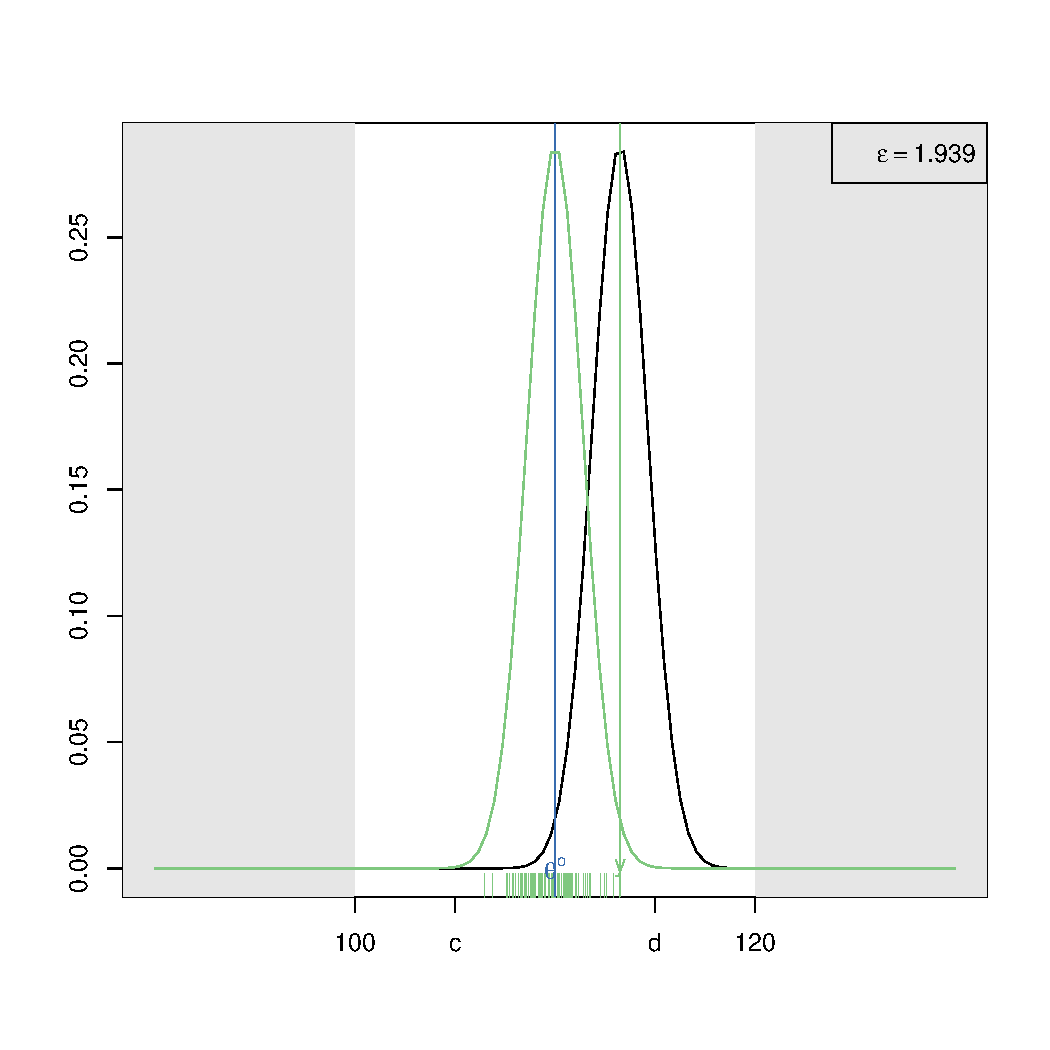
\includegraphics[scale=.35]{./Images/concentrate_36.pdf}}%
\only<38>{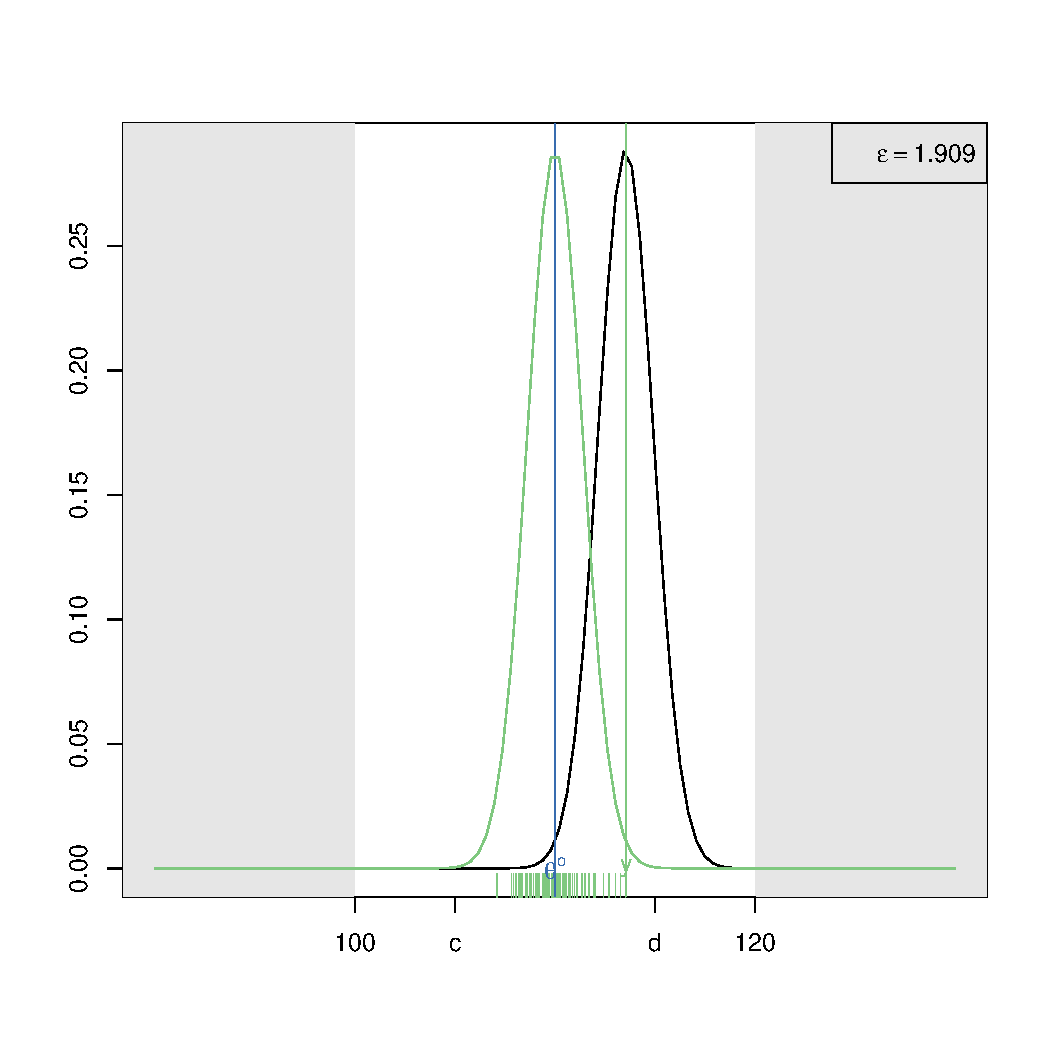
\includegraphics[scale=.35]{./Images/concentrate_37.pdf}}%
\only<39>{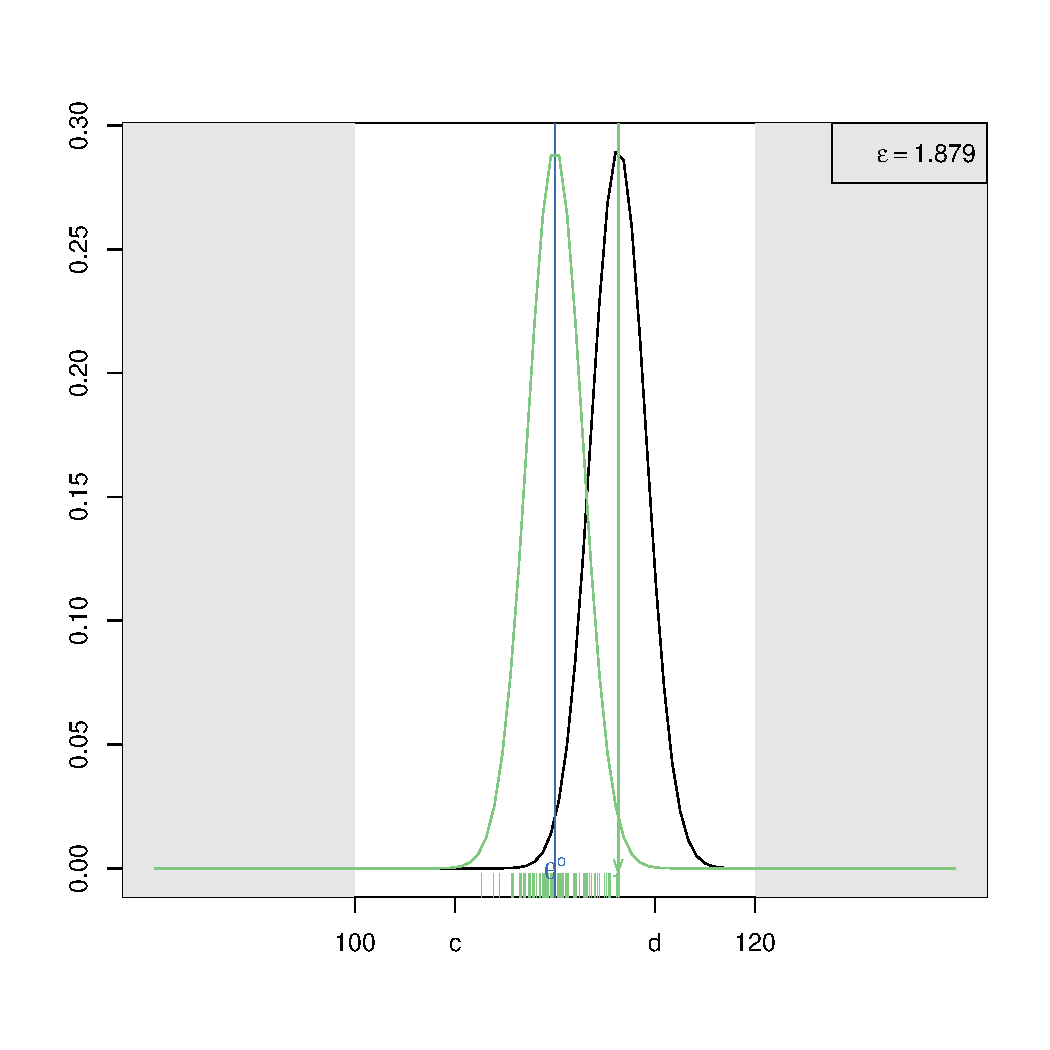
\includegraphics[scale=.35]{./Images/concentrate_38.pdf}}%
\only<40>{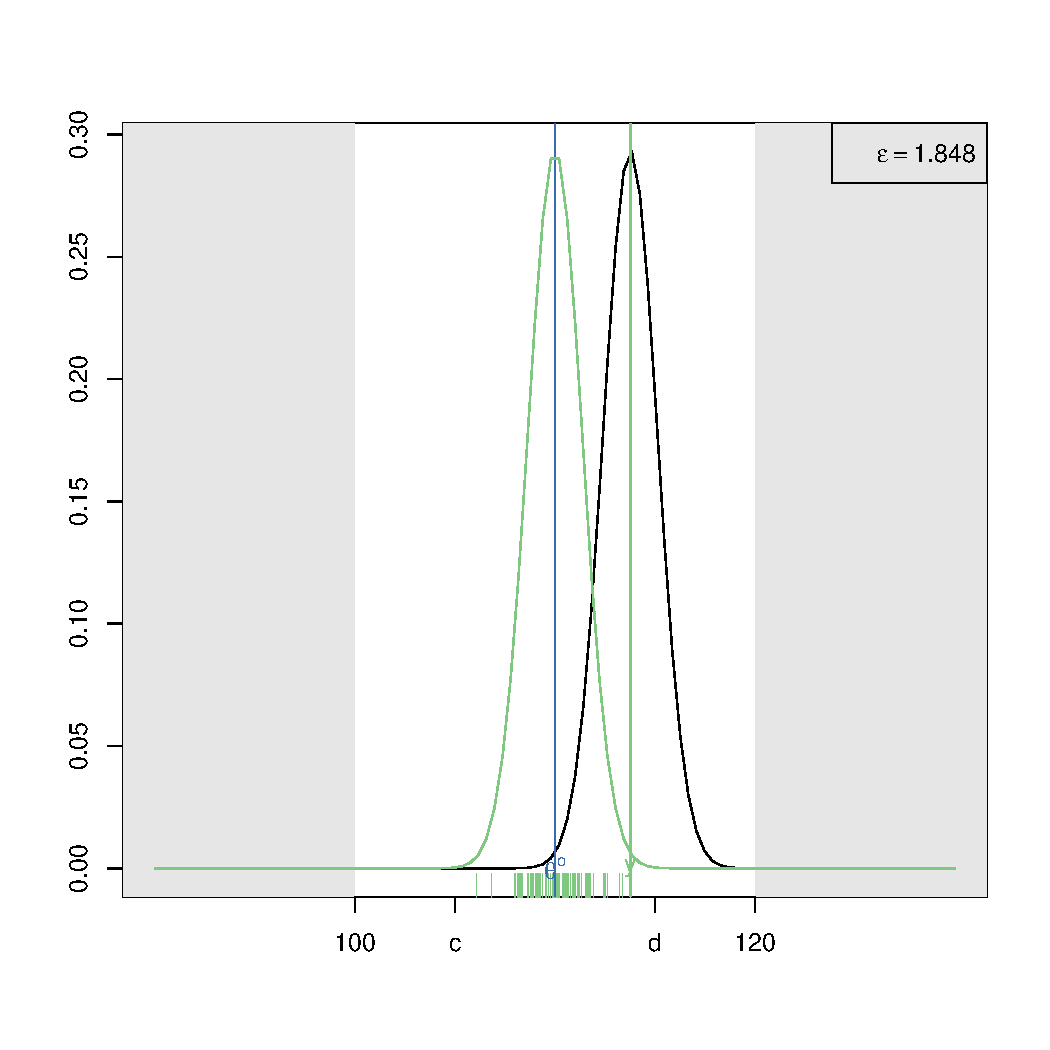
\includegraphics[scale=.35]{./Images/concentrate_39.pdf}}%
\only<41>{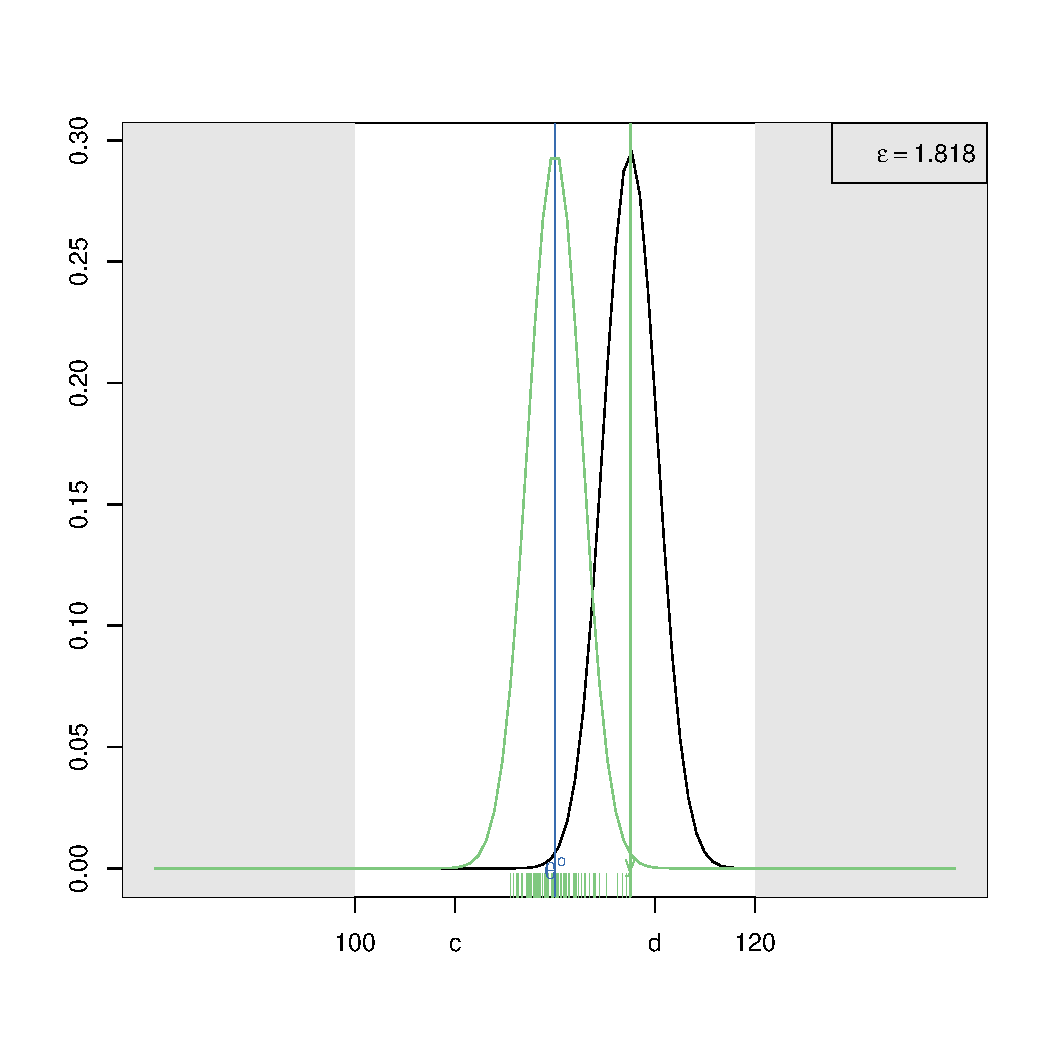
\includegraphics[scale=.35]{./Images/concentrate_40.pdf}}%
\only<42>{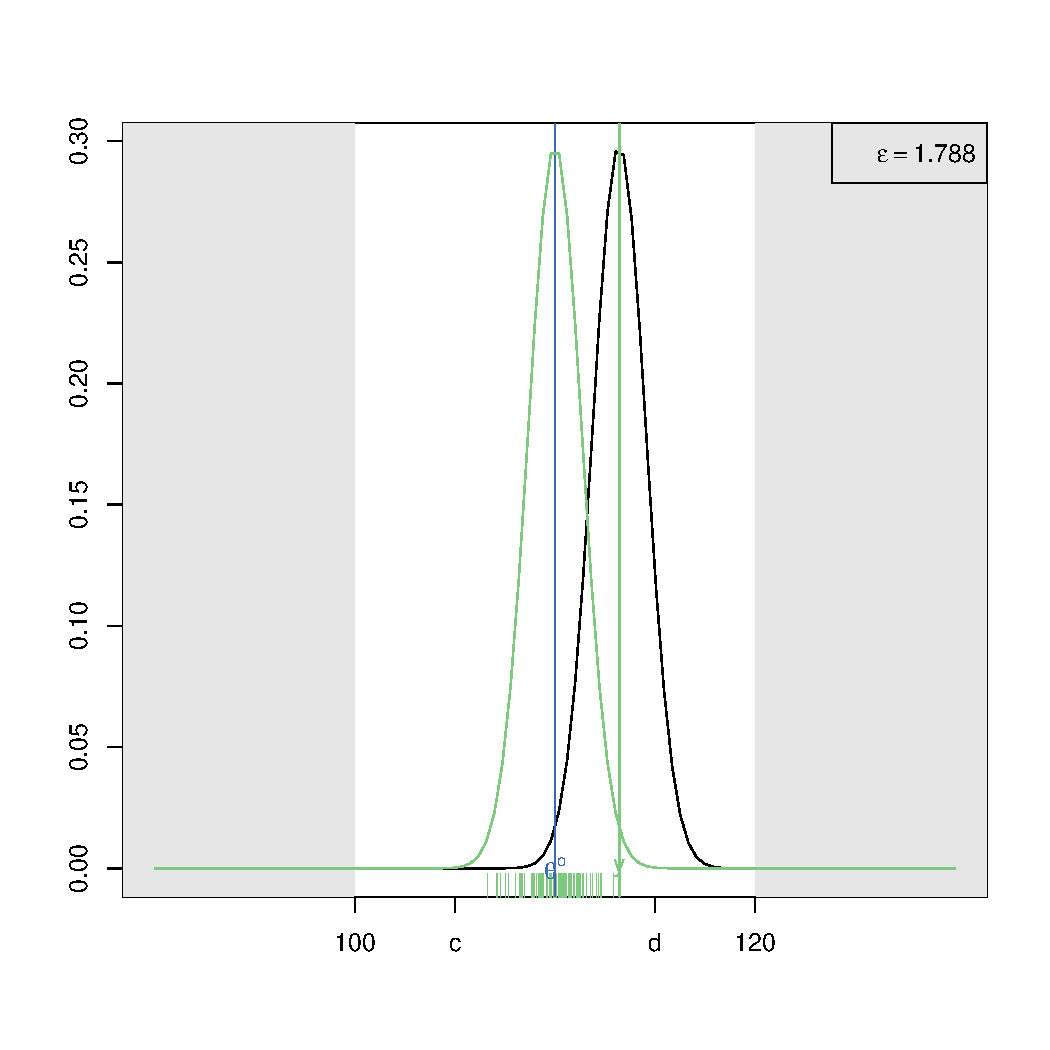
\includegraphics[scale=.35]{./Images/concentrate_41.pdf}}%
\only<43>{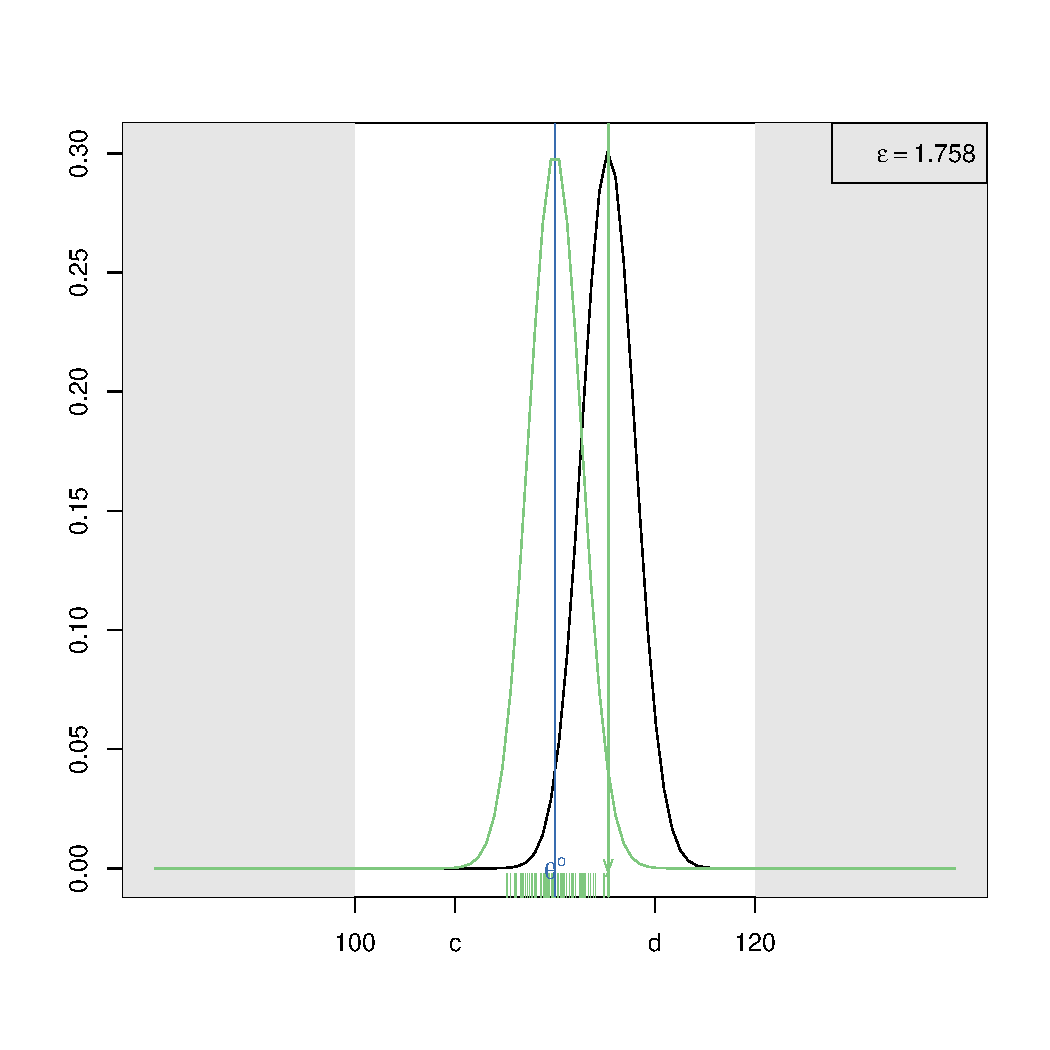
\includegraphics[scale=.35]{./Images/concentrate_42.pdf}}%
\only<44>{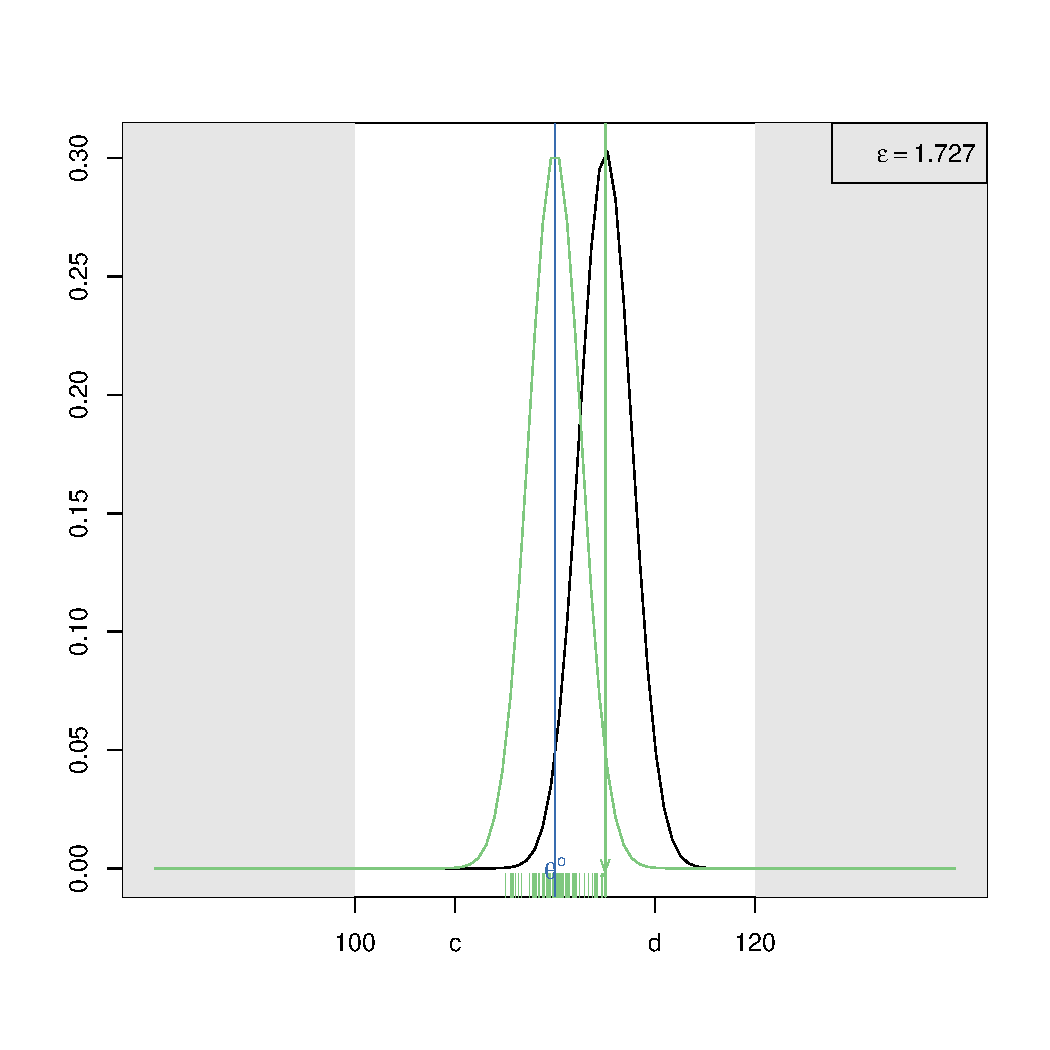
\includegraphics[scale=.35]{./Images/concentrate_43.pdf}}%
\only<45>{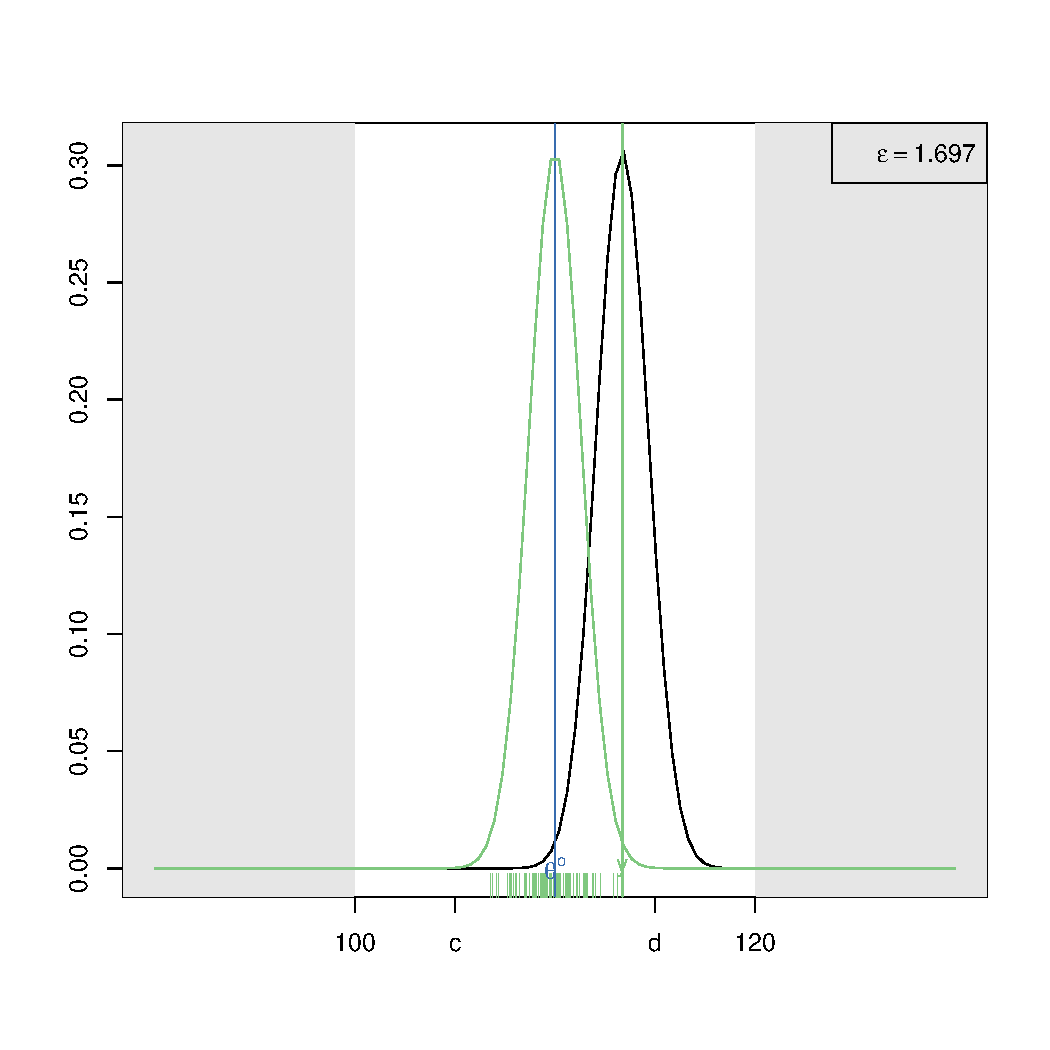
\includegraphics[scale=.35]{./Images/concentrate_44.pdf}}%
\only<46>{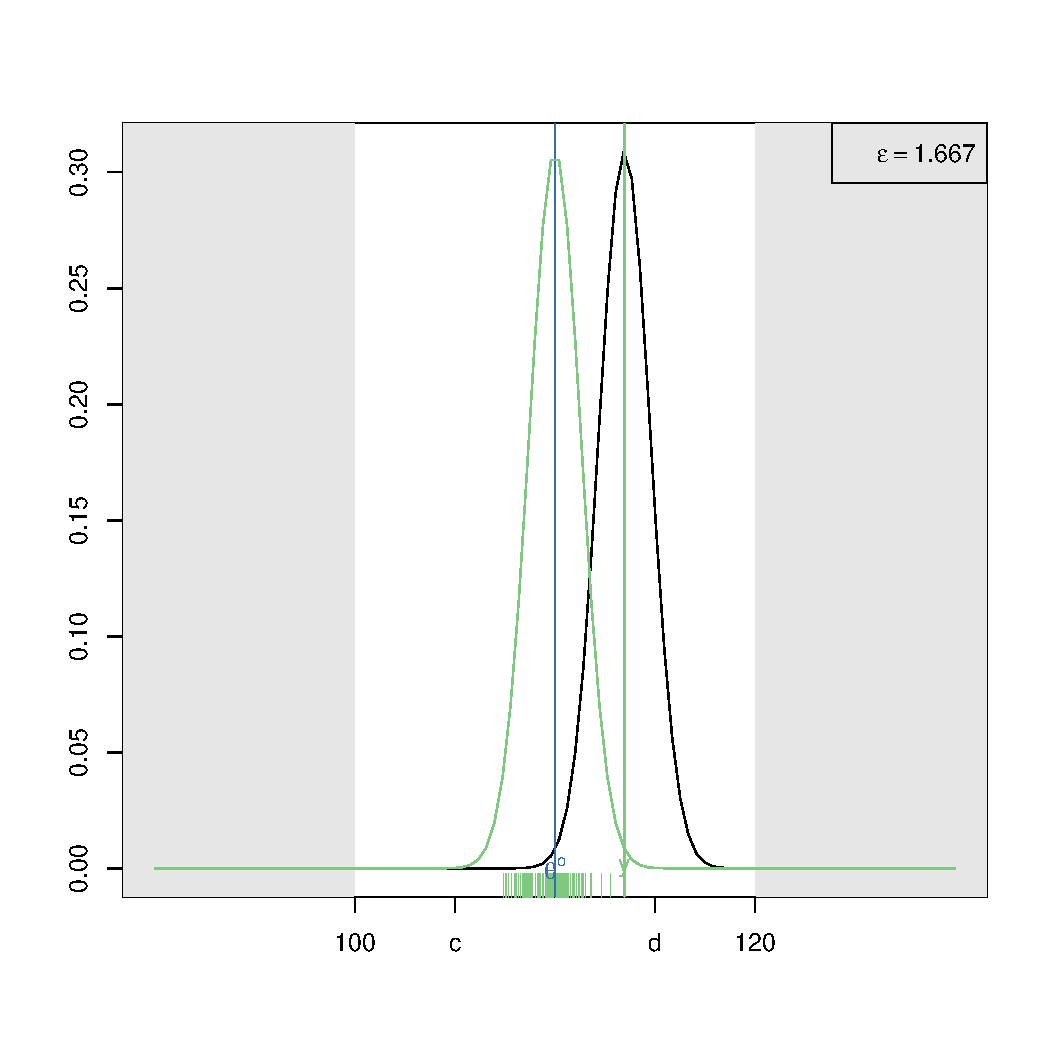
\includegraphics[scale=.35]{./Images/concentrate_45.pdf}}%
\only<47>{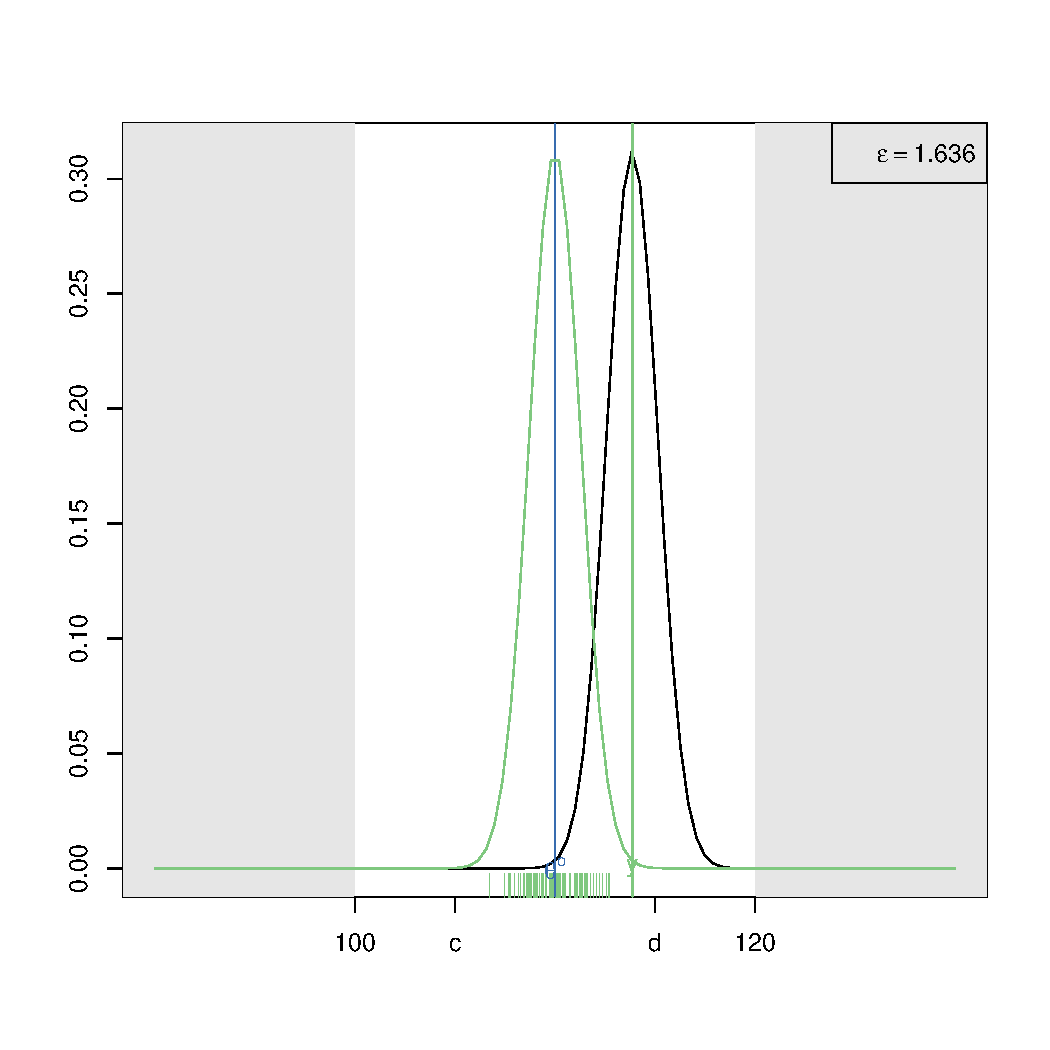
\includegraphics[scale=.35]{./Images/concentrate_46.pdf}}%
\only<48>{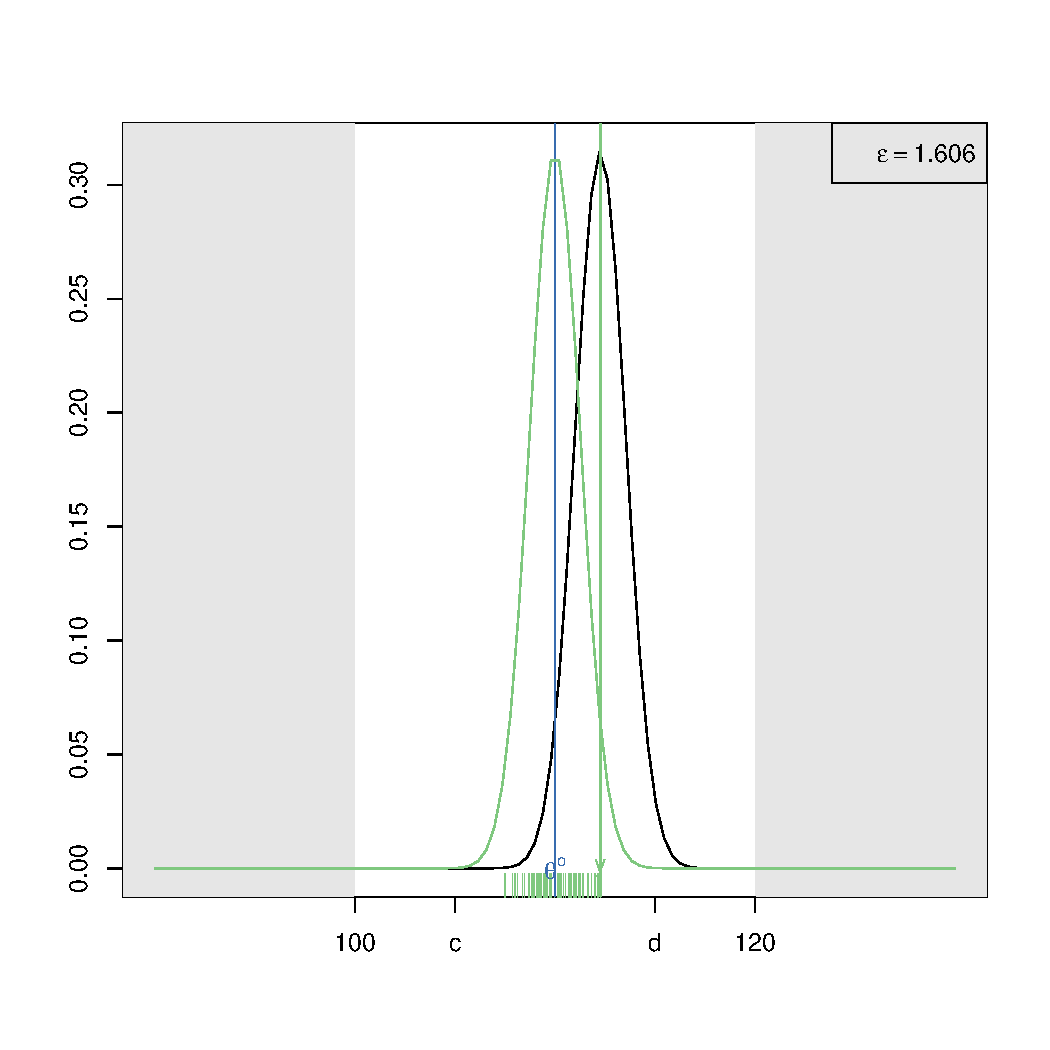
\includegraphics[scale=.35]{./Images/concentrate_47.pdf}}%
\only<49>{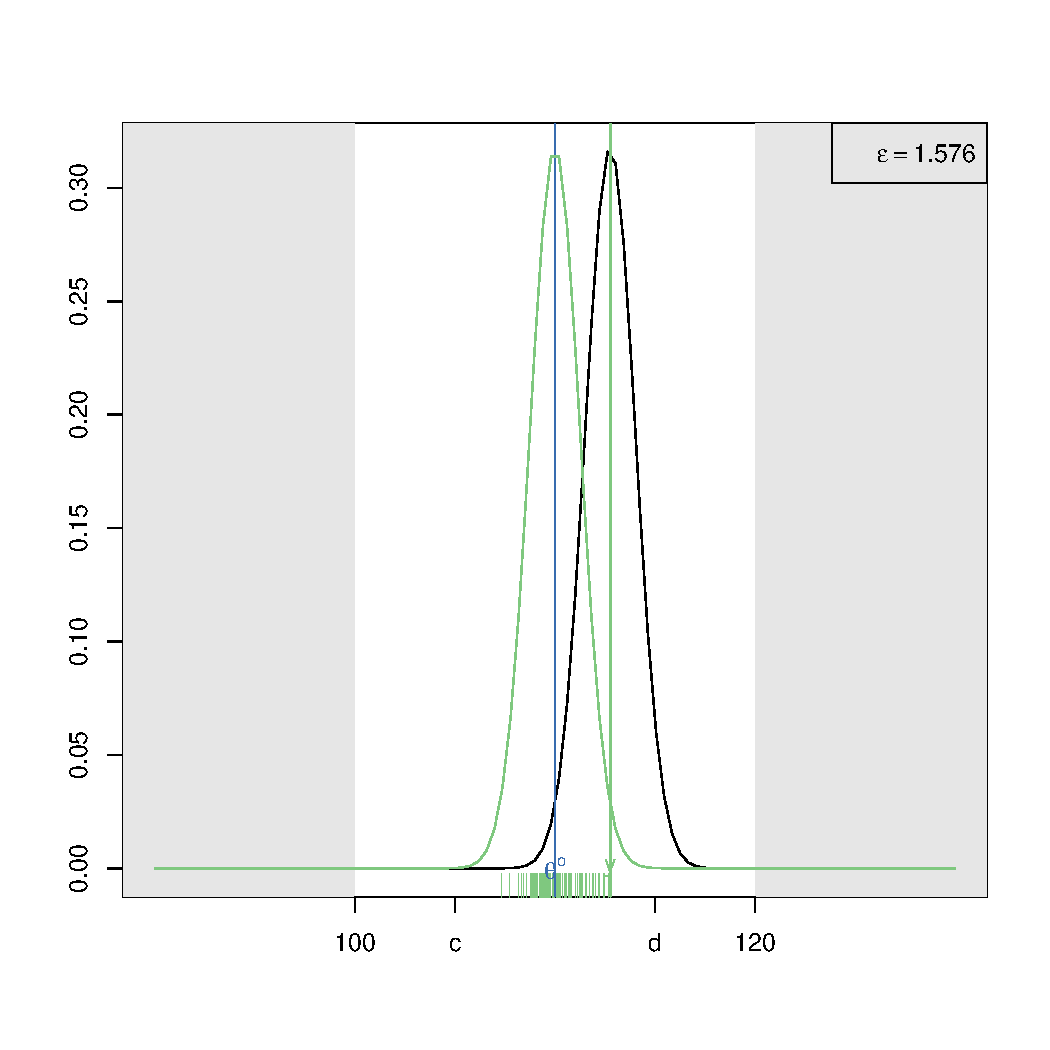
\includegraphics[scale=.35]{./Images/concentrate_48.pdf}}%
\only<50>{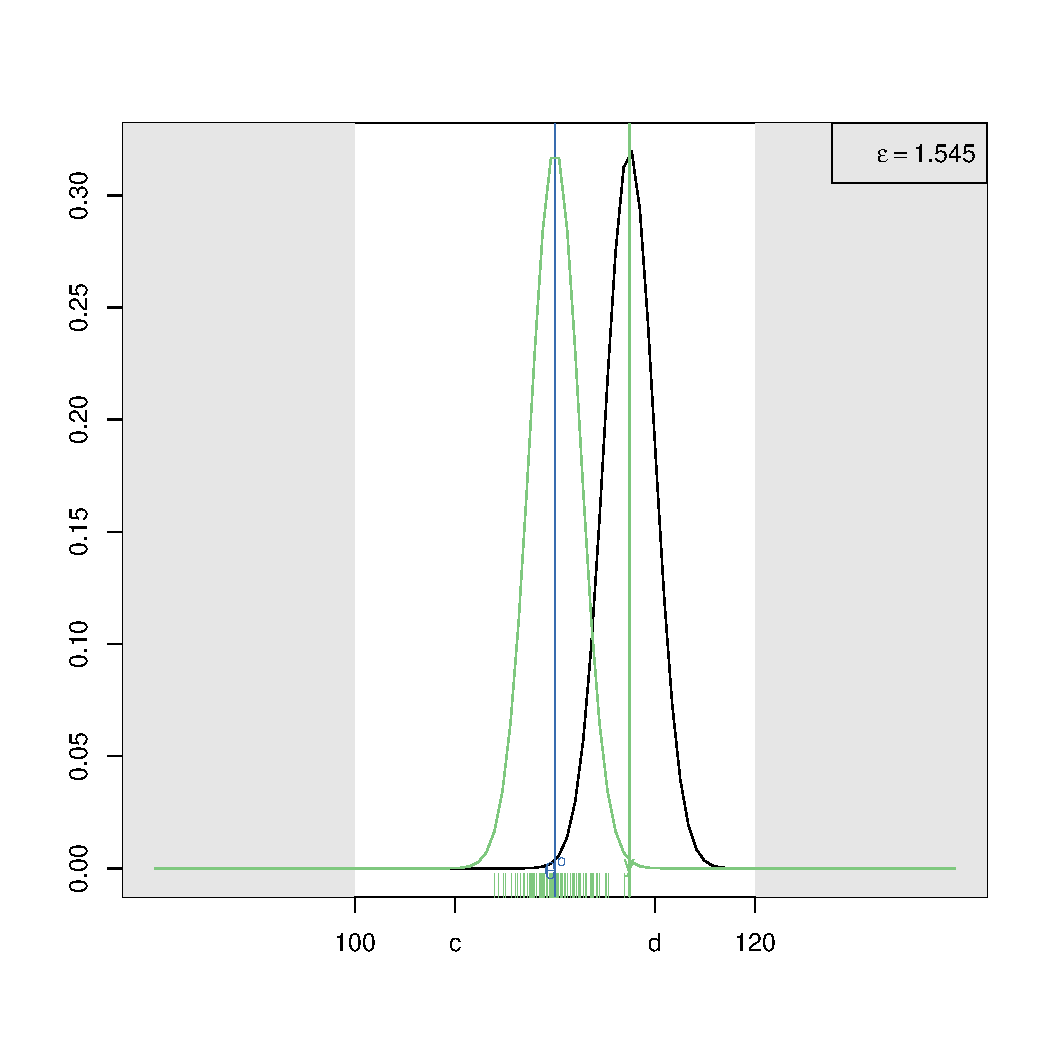
\includegraphics[scale=.35]{./Images/concentrate_49.pdf}}%
\only<51>{\includegraphics[scale=.35]{./Images/concentrate_50.pdf}}%
\only<52>{\includegraphics[scale=.35]{./Images/concentrate_51.pdf}}%
\only<53>{\includegraphics[scale=.35]{./Images/concentrate_52.pdf}}%
\only<54>{\includegraphics[scale=.35]{./Images/concentrate_53.pdf}}%
\only<55>{\includegraphics[scale=.35]{./Images/concentrate_54.pdf}}%
\only<56>{\includegraphics[scale=.35]{./Images/concentrate_55.pdf}}%
\only<57>{\includegraphics[scale=.35]{./Images/concentrate_56.pdf}}%
\only<58>{\includegraphics[scale=.35]{./Images/concentrate_57.pdf}}%
\only<59>{\includegraphics[scale=.35]{./Images/concentrate_58.pdf}}%
\only<60>{\includegraphics[scale=.35]{./Images/concentrate_59.pdf}}%
\only<61>{\includegraphics[scale=.35]{./Images/concentrate_60.pdf}}%
\only<62>{\includegraphics[scale=.35]{./Images/concentrate_61.pdf}}%
\only<63>{\includegraphics[scale=.35]{./Images/concentrate_62.pdf}}%
\only<64>{\includegraphics[scale=.35]{./Images/concentrate_63.pdf}}%
\only<65>{\includegraphics[scale=.35]{./Images/concentrate_64.pdf}}%
\only<66>{\includegraphics[scale=.35]{./Images/concentrate_65.pdf}}%
\only<67>{\includegraphics[scale=.35]{./Images/concentrate_66.pdf}}%
\only<68>{\includegraphics[scale=.35]{./Images/concentrate_67.pdf}}%
\only<69>{\includegraphics[scale=.35]{./Images/concentrate_68.pdf}}%
\only<70>{\includegraphics[scale=.35]{./Images/concentrate_69.pdf}}%
\only<71>{\includegraphics[scale=.35]{./Images/concentrate_70.pdf}}%
\only<72>{\includegraphics[scale=.35]{./Images/concentrate_71.pdf}}%
\only<73>{\includegraphics[scale=.35]{./Images/concentrate_72.pdf}}%
\only<74>{\includegraphics[scale=.35]{./Images/concentrate_73.pdf}}%
\only<75>{\includegraphics[scale=.35]{./Images/concentrate_74.pdf}}%
\only<76>{\includegraphics[scale=.35]{./Images/concentrate_75.pdf}}%
\only<77>{\includegraphics[scale=.35]{./Images/concentrate_76.pdf}}%
\only<78>{\includegraphics[scale=.35]{./Images/concentrate_77.pdf}}%
\only<79>{\includegraphics[scale=.35]{./Images/concentrate_78.pdf}}%
\only<80>{\includegraphics[scale=.35]{./Images/concentrate_79.pdf}}%
\only<81>{\includegraphics[scale=.35]{./Images/concentrate_80.pdf}}%
\only<82>{\includegraphics[scale=.35]{./Images/concentrate_81.pdf}}%
\only<83>{\includegraphics[scale=.35]{./Images/concentrate_82.pdf}}%
\only<84>{\includegraphics[scale=.35]{./Images/concentrate_83.pdf}}%
\only<85>{\includegraphics[scale=.35]{./Images/concentrate_84.pdf}}%
\only<86>{\includegraphics[scale=.35]{./Images/concentrate_85.pdf}}%
\only<87>{\includegraphics[scale=.35]{./Images/concentrate_86.pdf}}%
\only<88>{\includegraphics[scale=.35]{./Images/concentrate_87.pdf}}%
\only<89>{\includegraphics[scale=.35]{./Images/concentrate_88.pdf}}%
\only<90>{\includegraphics[scale=.35]{./Images/concentrate_89.pdf}}%
\only<91>{\includegraphics[scale=.35]{./Images/concentrate_90.pdf}}%
\only<92>{\includegraphics[scale=.35]{./Images/concentrate_91.pdf}}%
\only<93>{\includegraphics[scale=.35]{./Images/concentrate_92.pdf}}%
\only<94>{\includegraphics[scale=.35]{./Images/concentrate_93.pdf}}%
\only<95>{\includegraphics[scale=.35]{./Images/concentrate_94.pdf}}%
\only<96>{\includegraphics[scale=.35]{./Images/concentrate_95.pdf}}%
\only<97>{\includegraphics[scale=.35]{./Images/concentrate_96.pdf}}%
\only<98>{\includegraphics[scale=.35]{./Images/concentrate_97.pdf}}%
\only<99>{\includegraphics[scale=.35]{./Images/concentrate_98.pdf}}%
\only<100>{\includegraphics[scale=.35]{./Images/concentrate_99.pdf}}}
\end{frame}
% --------------------------------------------------------------------
% <<Intro-F9>>
% --------------------------------------------------------------------
\bframeVL{1-12}{12}
  \frametitle{{\dgrau A glimpse to the essential:} exact posterior  concentration}
\begin{overlayarea}{\textwidth}{.9\textheight}
\begin{columns}\begin{column}[T]{.6\textwidth}%
  Given prior $P_{\RvSo}$ {\dronly{1-}find $\Ra_\ObSoNoL\dwonly{1} \to 0$}\invisible<1>{ as $\ObSoNoL\to 0$ such that
  for $P_{\TrSo}=P_{\ObSo|\RvSo=\TrSo}$}
\begin{dbListeT}[\setListeL{2ex}{2ex}{5ex}{5ex}] 
   \item<2-> $P_{\RvSo|\ObSo} ( \normV{\RvSo-\TrSo}\lesssim {\dr\Ra_\ObSoNoL})\stackrel{P_{\TrSo}}{\to} 1$
   \item<6-> $P_{\RvSo|\ObSo} ( \normV{\RvSo-\TrSo}\gtrsim {\dr\Ra_\ObSoNoL})\stackrel{P_{\TrSo}}{\to} 1$
   \end{dbListeT}
\mywboxinvisible{-9}{{\dgrau Remarks:}
\begin{dshListeT}[\setListeL{2ex}{2ex}{5ex}{5ex}] 
 \item<10-> $\dr\Ra_\ObSoNoL$ depends on the prior
  \item<11-> $\dr\Ra_\ObSoNoL$ might be arbitrarily slow
  \item<12-> consistency could fail
  \end{dshListeT}}
\end{column}\begin{column}[T]{.4\textwidth}%
\hspace*{4ex}\includegraphics<1>[scale=.8]{./Images/reg.31}%
\includegraphics<2>[scale=.8]{./Images/reg.31}%
\includegraphics<3>[scale=.8]{./Images/reg.32}%
\includegraphics<4>[scale=.8]{./Images/reg.33}%
\includegraphics<5>[scale=.8]{./Images/reg.34}%
\includegraphics<6>[scale=.8]{./Images/reg.35}%
\includegraphics<7>[scale=.8]{./Images/reg.36}%
\includegraphics<8>[scale=.8]{./Images/reg.37}%
\includegraphics<9->[scale=.8]{./Images/reg.38}%
%\begin{textblock}{6}(2,14.5) \only<1->{{\db Parameter of interest}}\end{textblock} 
%\begin{textblock}{6}(9.5,14.5)\only<1->{{\db Transformed  parameter}}\end{textblock} 
\end{column}
\end{columns}
\end{overlayarea}
\end{frame}


% --------------------------------------------------------------------
% <<References>>
% --------------------------------------------------------------------
\begin{frame}
\frametitle{}
{\small{\begin{thebibliography}{10}       
\beamertemplatearticlebibitems

\bibitem{[1]}\dg {S. Ghosal, J.K. Ghosh and  A.W. Van Der Vaart} (2000)
{\ds\it Convergence rates of posterior distributions.}
{\ds The Annals of Statistics 28(2):500–531}

\bibitem{[2]}\dg {X. Shen and L. Wasserman.} (2001) 
{\ds\it Rates of convergence of posterior distributions.}
{\ds The Annals of Statistics, 29:687–714}


\bibitem{[3]}\dg {B. Knapik, A. Van der Vaart, and J. Van Zanten} (2011) 
{\ds\it Bayesian inverse problems with gaussian priors.}
{\ds The Annals of Statistics, 39:2626–2657}

\bibitem{[4]}\dg {J. Arbel, G. Gayraud and J. Rousseau} (2013) 
{\ds\it Bayesian optimal adaptive estimation using a sieve prior.}
 {\ds Scandinavian Jounral of Statistics, 40:549--570}

% \bibitem{[5]}\dg {B. Knapik, B. Szabó, A. Van der Vaart, and J. Van
%     Zanten} (2014)
% {\ds\it Bayes procedures for adaptive inference in inverse problems
%   for the white noise model.}
% {\ds Preprint, arXiv:1209.3628v2}

\bibitem{[6]}\dg {K. Ray} (2013)
{\ds\it Bayesian inverse problems with non-conjugate priors.} 
{\ds Electronic Journal of Statistics, 7: 2516–2549}

\bibitem{[7]}\dg {M. Hoffmann, J. Rousseau  and  J. Schmidt-Hieber} (2015) {\ds\it On adpative posterior concentration rates.} 
{\ds The Annals of Statistics, 43:5,2259--2295}

 \bibitem{[8]}\dg  {I. Castillo} (2008) 
{\ds \it Lower bounds for posterior rates with Gaussian process  priors.}
{\ds Electronic Journal of Statistics, 2:1281-1299}
\end{thebibliography}}}
\end{frame}


% --------------------------------------------------------------------
% <<Intro-F10>>
% --------------------------------------------------------------------
\bframeVL{1-3}{3}[label=Op]
\frametitle{{\rudicolor  Objective:} exact posterior concentration}
\begin{rudiListeS}[\setListeL{4ex}{2ex}{5ex}{5ex}] 
\item Construct   a family  $\{P_{\DiRvSo}\}_{\Di}$ of prior
  distributions with\\[1ex]
{\dr exact} posterior  concentration $\eRa^{\eDi}:=\eRa^{\eDi}(\TrSo)$ for $\TrSo\in\cSo$,
  i.e.,
\[\lim_{\ObSoNoL\to0} \Ex_{\TrSo}
P_{\hspace*{-.8ex}\DiRvSo[\eDi]|\ObSo}\Bigl(\eRa^{\eDi} \lesssim
\normV{\DiRvSo[\eDi]-\TrSo}^2\lesssim \eRa^{\eDi}\Bigr)=1;\]
\begin{rudiListeT}[\setListeL{2ex}{5ex}{2ex}{0ex}] 
\item<2-> Consider for a given $\TrSo\in\cSo$ the {\rudicolor oracle} rate
\[\treRa:=\treRa(\TrSo):=\inf_{\Di}\,\eRa^{\Di}(\TrSo).  \]
% \item<5-> Consider for a given $\cwSo\subset\cSo$  the {\rudicolor minimax} rate
% \[\oeRa:=\oeRa(\wSo):=\inf_{\tSo}\sup_{\TrSo\in\cwSo}\Ex_{\TrSo}\normV{\tSo-\TrSo}^2.  \]
\item<3-> Consider for a given $\cwSo\subset\cSo$  the {\rudicolor minimax} rate
\[\oeRa:=\oeRa(\wSo):=\inf_{\Di}\sup_{\TrSo\in\cwSo}\eRa^{\Di}(\TrSo).  \]
\end{rudiListeT}
\end{rudiListeS}
\end{frame}

% --------------------------------------------------------------------
% <<Intro-F11>>
% --------------------------------------------------------------------
\bframeVL{1-2}{2}[label=OPC]
\frametitle{{\rudicolor Objective:} optimal prior choice}
\begin{rudiListeS}[\setListeL{4ex}{2ex}{5ex}{5ex}] 
\item A  sub-family $\{P_{\hspace*{-.8ex}\DiRvSo[\treDi]}\}_{\treDi}$
  with {\rudicolor exact} posterior  concentration   $\treRa$, i.e.
\[\lim_{\ObSoNoL\to0} \Ex_{\TrSo} P_{\hspace*{-.8ex}\DiRvSo[\treDi]|\ObSo}\Bigl(\treRa \lesssim \normV{\DiRvSo[\treDi]-\TrSo}^2\lesssim \treRa  \Bigr)=1, \]  
is called {\rudicolor oracle} prior  and {\dr adaptive} if it
does not depend on $\TrSo$.
% \item<3-> and  a Bayes estimate
%   $\hDiSo[\treDi]:=\Ex[\DiRvSo[\treDi]|\ObSo]$ satisfying
%   \[  \Ex_{\TrSo}\normV{\hDiSo[\treDi]-\TrSo}^2\lesssim \treRa \]   
% is called ``oracle Bayes estimate''.
% \item Consider for given $\cwSo\subset\cSo$  the minimax rate
% \[\oeRa:=\oeRa(\wSo):=\inf_{\tSo}\sup_{\TrSo\in\cwSo}\Ex_{\TrSo}\normV{\tSo-\TrSo}^2.  \]
\item<2-> A sub-family $\{P_{\hspace*{-.8ex}\DiRvSo[\oeDi]}\}_{\oeDi}$
  with {\rudicolor exact} posterior
  concentration  $\oeRa$, i.e.
\[\lim_{\ObSoNoL\to0}  \inf_{\TrSo\in\cwSo} \Ex_{\TrSo}P_{\hspace*{-.8ex}\DiRvSo[\oeDi]|\ObSo}\Bigl(\oeRa\lesssim
  \normV{\DiRvSo[\oeDi]-\TrSo}^2\lesssim \oeRa  \Bigr)=1.
  \]  
is called {\rudicolor minimax} prior and {\dr adaptive} if it
depends not on $\cwSo$.
% \item<3-> and  a Bayes estimate
%   $\hDiSo[\oeDi]:=\Ex[\DiRvSo[\oeDi]|\ObSo]$ satisfying
%   \[ \sup_{\TrSo\in\cwSo} \Ex_{\TrSo}\normV{\hDiSo[\oeDi]-\TrSo}^2\lesssim \oeRa \]   
% is called ``minimax Bayes estimate''.
\end{rudiListeS}
\end{frame}



% % --------------------------------------------------------------------
% % <<Intro-F1>>
% % --------------------------------------------------------------------
% \bframeVL{22-34}{34}[label=IIP]
% \frametitle{\only<22-31>{{\dgrau A glimpse to the
%     essential:} {{\dwonly{22-27}statistical} {\dwonly{22-24}inverse
%     problem}}}\only<32-35>{{\dgrau Considered framework:} ill-posed
% inverse problem}}
% \centerline{%
% \includegraphics<22>[scale=.8]{./Images/inv.1}%
% \includegraphics<23>[scale=.8]{./Images/inv.2}%
% \includegraphics<24>[scale=.8]{./Images/inv.3}%
% \includegraphics<25>[scale=.8]{./Images/inv.4}%
% %\includegraphics<30>[scale=.9]{./Images/inv.5}
% \includegraphics<26>[scale=.8]{./Images/inv.6}%
% \includegraphics<27>[scale=.8]{./Images/inv.7}%
% \includegraphics<28>[scale=.8]{./Images/inv.8}%
% \includegraphics<29>[scale=.8]{./Images/inv.9}%
% \includegraphics<30>[scale=.8]{./Images/inv.10}%
% \includegraphics<31>[scale=.8]{./Images/inv.11}%
% \includegraphics<32>[scale=.8]{./Images/inv.12}%
% \includegraphics<33>[scale=.8]{./Images/inv.13}%
% \includegraphics<34,35>[scale=.8]{./Images/inv.14}%
% \includegraphics<35>[scale=.8]{./Images/inv.15}%
% }
% \begin{textblock}{6}(2,14.5) \only<22->{{\dgrau Function of interest}}\end{textblock} 
% \begin{textblock}{6}(9.5,14.5)\only<24->{{\dgrau Transformed  function}}\end{textblock} 
% \begin{textblock}{6}(7,4.5)\only<26>{{\db Existence
%       ?}}\only<27>{{\db Identified ?}}\only<29-31>{{\db Stability ?}}\end{textblock} 
% \begin{textblock}{6}(6.3,10.5)\only<32->{{\dr
%       Stability: no!}} \end{textblock} 
% \begin{textblock}{6}(6.3,6.9)\only<33->{{\dg Identified: assumed.}} \end{textblock} 
% \begin{textblock}{6}(6.3,4.5)\only<34>{{\dg Existence:
%       assumed.}} \end{textblock} 

% \begin{textblock}{6}(11.5,11)\small\only<28>{{\dgrau Estimator}}\end{textblock} 
% \begin{textblock}{6}(3,11)\small\only<28>{{\dgrau Estimator}}\end{textblock} 
% % \begin{textblock}{6}(2,14.5) \only<22->{{\dgrau Parameter of interest}}\end{textblock} 
% % \begin{textblock}{6}(9.5,14.5)\only<24->{{\dgrau Transformed  parameter}}\end{textblock} 
% % \begin{textblock}{6}(7,4.5)\only<26,34>{{\dgrau Existence ?}}\only<27,33>{{\dg Identified ?}}\only<29-32>{{\dg Stability ?}} \end{textblock} 
% % \begin{textblock}{6}(10.8,11)\small\only<28>{{\dg\lq\lq Measurement\rq\rq}}\end{textblock} 
% % \begin{textblock}{6}(3,11)\small\only<28>{{\dg Estimator}}\end{textblock} 
% \end{frame}
% % --------------------------------------------------------------------
% % <<Intro-F2>>
% % --------------------------------------------------------------------
% \bframeVL{1-5}{5}
% \frametitle{{\dgrau Background:} analytical inverse problem}
% Consider $(\colF,\skalar)$, $(\colG,\skalar)$ and
% $\colT:\colF\to\colG$ linear\\[1.5ex]
% \hspace*{5ex}{\xymatrix{
% \colf \ar@{|->}[r]^\colT\only<3->{\ar@{<->}[d]}& \colg \only<5->{\ar@{<->}[d]}\\
% \uncover<3->{(\alt<3>{\skalarV{\colf,\colbasF_j}}{\coltheta_j})_{j}}\only<5->{\ar@{|->}[r]^\collambda}& 
% \uncover<5->{(\collambda_j\coltheta_j)_{j}}}}\hfill\\[1.5ex]
% \mywboxinvisible{-1}{{special case}
%  $\colT$ permits a singular value decomposition  
% \begin{rudiListeS}[\setListeL{2ex}{2ex}{5ex}{5ex}] 
%   \item<2-> Singular values $\collambda:=(\collambda_j)_{j}$
%   \item<2-> Eigenfunctions $\{\colbasF_j\}_{j}$ and
%     $\{\colbasG_j\}_{j}$ ONB of $\colF$ and $\colG$, resp.
%   \end{rudiListeS}}

% \mywboxinvisible{-2}{{\rudicolor Representation}
% \begin{rudiListeS}[\setListeL{2ex}{2ex}{5ex}{5ex}] 
%   \item<3-> $ \colf\in \colF$\uncover<4->{$\leftrightarrow \coltheta \in \colTheta:=\ell^2  $ via $\coltheta_j =\skalarV{\colf,\colbasF_j}$} 
%   \item<5-> Operator $\colT \leftrightarrow$ Multiplication with $\collambda$
%   \end{rudiListeS}}
% \end{frame}

% % --------------------------------------------------------------------
% % <<Intro-F16>>
% % --------------------------------------------------------------------
% \bframeVL{1-4}{4}
% \frametitle{{\dgrau A glimpse to the essential:} posterior
%   concentration rate}
% \centerline{%
% \includegraphics<1>[scale=.8]{./Images/reg.15}%
% \includegraphics<2>[scale=.8]{./Images/reg.16}%
% \includegraphics<3>[scale=.8]{./Images/reg.17}%
% \includegraphics<4>[scale=.8]{./Images/reg.18}%
% }
% \begin{textblock}{6}(2,14.5) \only<1->{{\db Parameter of interest}}\end{textblock} 
% %\begin{textblock}{6}(9.5,14.5)\only<1->{{\db Transformed  parameter}}\end{textblock} 
% \end{frame}



% % --------------------------------------------------------------------
% % <<Intro-F6>>
% % --------------------------------------------------------------------
% \bframeVL{1-3}{3}
% \frametitle{{\dgrau Frequentist point of view:} upper bound}
% \centerline{%
% \includegraphics<1>[scale=.8]{./Images/gssm.10}%
% \includegraphics<2>[scale=.8]{./Images/gssm.11}%
% \includegraphics<3>[scale=.8]{./Images/gssm.12}%
% }
% \begin{textblock}{6}(2,14.5) \only<1->{{\dgrau Parameter of interest}}\end{textblock} 
% \begin{textblock}{6}(9.5,14.5)\only<1->{{\dgrau Transformed  parameter}}\end{textblock} 
% \end{frame}
% % --------------------------------------------------------------------
% % <<Intro-F5>>
% % --------------------------------------------------------------------
% \bframeVL{1-3}{3}
% \frametitle{{\dgrau Frequentist point of view:} lower bound}
% \centerline{%
% \includegraphics<1>[scale=.8]{./Images/gssm.13}%
% \includegraphics<2>[scale=.8]{./Images/gssm.14}%
% \includegraphics<3>[scale=.8]{./Images/gssm.15}%
% }
% \begin{textblock}{6}(2,14.5) \only<1->{{\dgrau Parameter of interest}}\end{textblock} 
% \begin{textblock}{6}(9.5,14.5)\only<1->{{\dgrau Transformed  parameter}}\end{textblock} 
% \end{frame}
% % --------------------------------------------------------------------
% % <<Intro-F7>>
% % --------------------------------------------------------------------
% \bframeVL{1-4}{1}
% \frametitle{{\dgrau Frequentist point of view:} adaptation}
% \centerline{%
% \includegraphics<1>[scale=.8]{./Images/gssm.20}%
% %\includegraphics<2>[scale=.8]{./Images/reg.20}%
% \includegraphics<2>[scale=.8]{./Images/gssm.22}%
% \includegraphics<3>[scale=.8]{./Images/gssm.23}%
% \includegraphics<4>[scale=.8]{./Images/gssm.24}%
% }
% \begin{textblock}{6}(2,14.5) \only<1->{{\dgrau Parameter of interest}}\end{textblock} 
% \begin{textblock}{6}(9.5,14.5)\only<1->{{\dgrau Transformed  parameter}}\end{textblock} 
% \begin{textblock}{6}(10.8,11)\small\only<1>{{\dgrau Estimator}}\end{textblock} 
% \begin{textblock}{6}(6.4,11)\small\only<1>{{\db Data-driven}}\end{textblock} 
% \begin{textblock}{6}(1.8,11)\small\only<1>{{\db Data-driven}}\end{textblock} 
% \end{frame}




% % --------------------------------------------------------------------
% % <<Intro-F9>>
% % --------------------------------------------------------------------
% %%%%%%%%%%%%%%%%%%%%%
% \bframeVL{1-6}{10}
% \frametitle{{\dgrau A glimpse to the essential:} dimension reduction}
% %\mywbox{\centerline{{\db Reconstruct $\So$} given $\db\oIm =\Op\So + \sqrt\lnIm \nIm$ and $\db\oOp = \Op+ \sqrt\lnOp \nOp$.}}
% Introduce a  sieves sequence  $\dbonly{1}\Uz_1\subset\Uz_2\subset\cdots\subset\Uz_m\subset\cdots\subset\Hspace$.
% \begin{dbListeT}[\setListeL{5ex}{5ex}{2ex}{2ex}] 
% \item<2->  Consider a theoretical approximation  $\dbonly{2}\fSo_m\in \mHspace$  of $\fSo\in\Hspace$ and let %associated approximation error
%   \[\dbonly{2}\gb_m:=\sup\nolimits_{k\geq m}\normV{\fSo_k-\fSo}^2.\]
% \item<3-> Construct an {\dbonly{3}estimator $\hfSo_m$} of $\fSo_m$ based on  $\dbonly{3}\widehat{g}$\dwonly{3}, where 
%   \[\dbonly{4}\Ex_{\fSo}\normV{{\dbonly{4}\hfSo_m}-\fSo}^2\lesssim \dbonly{4}\gb_m(\fSo) + \Ex_{\fSo}\normV{\fSo_m-\hfSo_m}^2.\]
% \item<5-> Derive $\dbonly{5}\gv_m\geq
%   \Ex_{\fSo}\normV{\fSo_m-\hfSo_m}^2$\dwonly{5}, then \[\dbonly{6}
% \Ex_{\fSo}\normV{{\dbonly{6}\hfSo_m}-\fSo}^2\dbonly{6}\lesssim [\gb_m\vee\gv_m]=\max(\gb_m,\gv_m)\text{ for }\dbonly{6}m\geq1.\]
% % \item<7-> Optimal choice $\dbonly{7}\mopte{}:=\argmin\nolimits_m\set{\max( b_m^2,v_m)}$  \dwonly{7}gives  
% % \[\dbonly{8}\Rifes[]{{\dbonly{8}\hSoGa[\mopte{\lnIm,\lnOp}]}}{\cSo,\cOp}\lesssim \dbonly{8}\min\nolimits_m\set{\max( b_m^2,v_m)}=:\oRifes[]{\cSo,\cOp}\]
% % \dwonly{-8}which  establishes {\dbonly{9}minimax-optimality of $\hSoGa[\mopte{}]$}, if \[\dbonly{9}\inf\nolimits_{\tSo}\Rifes[]{{\dbonly{9}\tSo}}{\cSo,\cOp}\gtrsim \dbonly{9}\oRifes[]{\cSo,\cOp}.\]
% \end{dbListeT}
% \end{frame}
% % --------------------------------------------------------------------
% % <<Intro-F10>>
% % --------------------------------------------------------------------
% %%%%%%%%%%%%%%%%%%%%%
% \bframeVL{6-9}{10}
% \frametitle{{\dgrau A glimpse to the essential:} oracle inequality}
% %\mywbox{\centerline{{\db Reconstruct $\So$} given $\db\oIm =\Op\So + \sqrt\lnIm \nIm$ and $\db\oOp = \Op+ \sqrt\lnOp \nOp$.}}
% Introduce a  sieves sequence  $\dbonly{1}\Uz_1\subset\Uz_2\subset\cdots\subset\Uz_m\subset\cdots\subset\Hspace$.
% \begin{dbListeT}[\setListeL{5ex}{5ex}{2ex}{2ex}] 
% \item<5-> Let $\dbonly{5}\gb_m:=\sup\nolimits_{k\geq m}\normV{\fSo_k-\fSo}^2$ and  $\dbonly{5}\gv_m\geq \Ex_{\fSo}\normV{\fSo_m-\hfSo_m}^2$\dwonly{5}, then \[\dbonly{6}\Ex_{\fSo}\normV{{\dbonly{6}\hfSo_m}-\fSo}^2\dbonly{6}\lesssim [\gb_m\vee\gv_m]\text{ for }\dbonly{6}m\geq1.\]
% \item<7-> The {\rudicolor oracle} choice $\dbonly{7}m^{\TrSy}:=\argmin\nolimits_m\set{[\gb_m\vee\gv_m]}$  \dwonly{7}gives  
% \[\dbonly{8}\Ex_{\fSo}\normV{{\dbonly{8}\hfSo_{m^{\TrSy}}}-\fSo}^2\lesssim \dbonly{8}\min\nolimits_m\set{[\gb_m\vee\gv_m]}=:\treRa[](\fSo)\]
% \dwonly{-8}which  establishes an {\only<9>{\rudicolor}oracle} inequality,
% if \[\dbonly{9}\inf\nolimits_{m}\Ex_{\fSo}\normV{{\dbonly{9}\hfSo_{m}}-\fSo}^2\gtrsim \dbonly{9}\treRa[](\fSo).\]
% \end{dbListeT}
% \end{frame}
% % --------------------------------------------------------------------
% % <<Intro-F11>>
% % --------------------------------------------------------------------
% %%%%%%%%%%%%%%%%%%%%%
% \bframeVL{5-9}{10}
% \frametitle{{\dgrau A glimpse to the essential:} minimax optimality}
% %\mywbox{\centerline{{\db Reconstruct $\So$} given $\db\oIm =\Op\So + \sqrt\lnIm \nIm$ and $\db\oOp = \Op+ \sqrt\lnOp \nOp$.}}
% Introduce a  sieves sequence  $\dbonly{1}\Uz_1\subset\Uz_2\subset\cdots\subset\Uz_m\subset\cdots\subset\Hspace_{\dbonly{5}\ga}$.
% \begin{dbListeT}[\setListeL{5ex}{5ex}{2ex}{2ex}] 
% \item<5-> Given $\mathcal{F}_{\dbonly{5}\ga}$ derive $\dbonly{5,6}\ga_m\geq \gb_m(\fSo)$\dwonly{5}
%   and  $\dbonly{6}\gv_m\geq
%   \Ex_{\fSo}\normV{\fSo_m-\hfSo_m}^2$\dwonly{5}, then \[\dbonly{6}\Ra[\,{\dbonly{6}\hfSo_m}\,|\,\mathcal{F}_{\ga}\,]
% \dbonly{6}\lesssim [\ga_m\vee\gv_m]\text{ for }\dbonly{6}m\geq1.\]
% \item<7-> The {\rudicolor minimax} choice $\dbonly{7}m^{\OpSy}:=\argmin\nolimits_m\set{[\ga_m\vee\gv_m]}$  \dwonly{7}gives  
% \[\dbonly{8}\Ra[\,{\dbonly{6}\hfSo_{m^{\OpSy}}}\,|\,\mathcal{F}_{\ga}\,]\lesssim \dbonly{8}\min\nolimits_m\set{[\ga_m\vee\gv_m]}=:\oeRa[](\ga)\]
% \dwonly{-8}which  establishes {\only<9>{\rudicolor minimax}} optimality of
%   $\hfSo_{m^{\OpSy}}$, if \[\dbonly{9}\inf\nolimits_{\tfSo}\Ra[\,{\dbonly{9}\tfSo}\,|\,\mathcal{F}_{\ga}\,]
% \gtrsim \dbonly{9}\oeRa[](\ga).\]
% \end{dbListeT}
% \end{frame}
% % --------------------------------------------------------------------
% % <<Intro-F12>>
% % --------------------------------------------------------------------
% %%%%%%%%%%%%%%%%%%%%%
% \bframeVL{1-4,6}{7}
% \frametitle{{\dgrau A glimpse to the essential:} adaptation}
% Introduce a  sieves sequence $\Uz_1\subset\Uz_2\subset\cdots\subset\Uz_m\subset\cdots\subset\Hspace$.
% \begin{dbListeT}[\setListeL{5ex}{5ex}{2ex}{2ex}] 
% % \item  Let $\dbonly{1}\SoGa\in \mHspace$ be a theoretical approximation of $\So\in\Hspace$.%  with %associated approximation error
% %   % \[\bias_m(\So):=\sup\nolimits_{k\geq m}\dist(\SoGa[k],\So).\]
% \item Construct an {\dbonly{1}estimator $\hfSo_{\dbonly{2}m}$} of $\fSo_{\dbonly{2}m}\in \mHspace$ based on  $\dbonly{1}\widehat{g}$.
% \item<2-> Select  $\dbonly{2}\only<1-2>{m}\only<3->{\whm}$ by using a {\dbonly{2}penalised minimum contrast criterion}\dwonly{2}%\\[.7ex]%
% $${\dbonly{3,7}\whm}:=\argmin_{1\leq m\leq \dbonly{3}\dronly{6}M}  \big\{\only<3>{\mbox{\dbonly{3,5,7}Contrast}_m}\only<4->{{\dbonly{4,7}-\normV{\hfSo_{m}}^2}}+{\dbonly{3}\dronly{6}\pen}_m\big\}.$$
% % \item<4-> Measure its performance: $\dbonly{4,7} \Ex_{\fSo}{\dbonly{5}\normV{\hfSo_{\whm}-\fSo}^2}$ \dwonly{4}then%\\[1ex]
% % $$\mbox{\dbonly{5,7}Contrast}_m:=\max_{m\leq k\leq \dronly{6}M}  \set{ {\dbonly{5,7}\normV{\hfSo_k-\hfSo_m}^2} - {\dronly{6}\pen}_k}$$
% % {\scriptsize which  is inspired by a recent work of Goldenshluger and Lepski [2011].}
% \end{dbListeT}
% \end{frame}
% % % --------------------------------------------------------------------
% % % <<Intro-F13>>
% % % --------------------------------------------------------------------
% % \setbeamertemplate{footline} 
% % {% 
% % \begin{beamercolorbox}[ht=2.5ex,dp=1.5ex]{footbox} 
% % %\hspace*{2ex} Jan \textbf{\sc Johannes} (UCL)\hfill\bf\insertframenumber/\inserttotalframenumber\hspace*{2ex}
% % \hspace*{2ex} \dnav\hfill\bf{\tiny\hyperlink{SkipProof1}{\insertskipsymbol}}\insertframenumber/\inserttotalframenumber\hspace*{2ex}
% % \end{beamercolorbox}% 
% % }
% % %%%%%%%%%%%%%%%%%%%%%
% % \bframeVL{1-11}{7}
% % \frametitle{\dgrau Key argument}
% % \hfill\\[-7ex]
% % \begin{overlayarea}{\textwidth}{.25\textheight}%
% % \begin{multline*}%
% % {\dronly{8-9 }\whm:=\argmin_{1\leq m\leq {M}}\big\{\mbox{Contrast}_m + \pen_m\big\}}\\[-2ex]
% % \hfill {\dronly{5,7}Contrast_m:=\max_{m\leq k\leq {M}}  \set{
% %   {\dronly{1}\normV{\widehat{f}_{k}-\widehat{f}_{m}}^2} -\pen_k}}
% % \end{multline*}
% % \end{overlayarea}
% % \begin{overlayarea}{\textwidth}{.8\textheight}%
% % \hrule\vspace{.5em}
% % \dwonly{1}For all $\dronly{10,11}1\leq m\leq M$ holds\dgronly{11}
% % \begin{multline*}
% % \only<1-3>{%
% % {\dronly{1}\normV{\widehat{f}_{{\dronly{2}\whm}}-f}^{{\dwonly{1-2}\dronly{3}2}}}\dwonly{1}\leq
% % {\dwonly{1-2}\dronly{3}3\Bigl(}\normV{\widehat{f}_{{\dronly{2}\whm}}-\widehat{f}_{{\dronly{2}\whm\wedge m}}}^{{\dwonly{-2}\dronly{3}2}} +
% % \normV{\widehat{f}_{{\dronly{2}m}}-\widehat{f}_{{\dronly{2}\whm\wedge m}}}^{{\dwonly{-2}\dronly{3}2}} + \normV{\widehat{f}_{{\dronly{2}m}}-f}^{{\dwonly{-2}\dronly{3}2}}{\dwonly{-2}\dronly{3}\Bigr)}}
% % \only<4->{%
% % {\dronly{10}\normV{\widehat{f}_{{\whm}}-f}^2}\leq
% % 3\Bigl(
% % {\dronly{4-5}\underbrace{\normV{\widehat{f}_{\whm}-\widehat{f}_{{\whm\wedge m}}}^2}_{{\dronly{4}\pm\pen_{\whm}}}} 
% % +\only<4-5>{\normV{\widehat{f}_{{m}}-\widehat{f}_{{\whm\wedge m}}}^2}
% % \only<6->{{\dronly{6-7}\underbrace{
% % \normV{\widehat{f}_{{m}}-\widehat{f}_{{\whm\wedge m}}}^2}_{{\dronly{3}\pm\pen_m}}}}
% % \Bigr) +3\,\normV{\widehat{f}_{{m}}-f}^2}
% % \hfill\\\hfill
% % \only<5-7>{\leq 3\Bigl({\dronly{5}\mbox{Contrast}_m + \pen_{\whm}}{\dwonly{-6}\dronly{7}+\mbox{Contrast}_{\whm} + \pen_m}\Bigr) + 3\,\normV{\widehat{f}_{{\dronly{2}m}}-f}^2}
% % \only<8->{\leq  3\Bigl(\mbox{Contrast}_m +
% %   {\dronly{8-9}\pen_{\whm}+\mbox{Contrast}_{\whm}} + \pen_m\Bigr) +
% %   3\,\normV{\widehat{f}_{{m}}-f}^2
% % \\\hfill\dwonly{1-8}
% % \leq 3\Bigl({\dronly{9}2\big\{}\mbox{Contrast}_{{\dronly{10}m}}+ \pen_{{\dronly{10}m}}{\dronly{9}\big\}}\Bigr) +
% %   3\,\normV{\widehat{f}_{{\dronly{10}m}}-f}^2}
% % \end{multline*}
% % \dwonly{-10}\dsonly{11}and applying several times the triangular inequality\\[-4ex]
% % \begin{equation*}
% % \dronly{11}
% % \normV{\widehat{f}_{{\whm}}-f}^{2}\lesssim [\gb_{{m}}\vee\pen_m]+\max_{m\leq k\leq M}\vectp{\normV{\widehat{f}_{k}-f_k}^2 -\tfrac{1}{6}\pen_k }
% % \end{equation*}
% % \end{overlayarea}
% % \end{frame}
% % \setbeamertemplate{footline} 
% % {% 
% % \begin{beamercolorbox}[ht=2.5ex,dp=1.5ex]{footbox} 
% % %\hspace*{2ex} Jan \textbf{\sc Johannes} (UCL)\hfill\bf\insertframenumber/\inserttotalframenumber\hspace*{2ex}
% % \hspace*{2ex} \dnav\hfill\bf\insertframenumber/\inserttotalframenumber\hspace*{2ex}
% % \end{beamercolorbox}% 
% % }
% % \hypertarget{SkipProof1}{}
% % --------------------------------------------------------------------
% % <<Intro-F14>>
% % --------------------------------------------------------------------
% %%%%%%%%%%%%%%%%%%%%%
% \bframeVL{1-4}{4}
% \frametitle{\dgrau Key argument}
% \hfill\\[-7ex]
% \begin{overlayarea}{\textwidth}{.25\textheight}%
% \begin{multline*}%
% {\dronly{0}\whm:=\argmin_{1\leq m\leq {M}}\big\{{-\normV{\hfSo_{m}}^2} + \pen_m\big\}}\hfill\\[-2ex]
% % \hfill {\dronly{0}Contrast_m:=\max_{m\leq k\leq {M}}  \set{
% %   {\dronly{0}\normV{\widehat{f}_{k}-\widehat{f}_{m}}^2} -\pen_k}}
% \end{multline*}
% \end{overlayarea}
% \begin{overlayarea}{\textwidth}{.8\textheight}%
% \hrule\vspace{.5em}
% For all $\dgonly{3-}1\leq m\leq M$ holds
% \begin{equation*}
% {\dsonly{1}\Ex_{\fSo}}\normV{\widehat{f}_{{\whm}}-f}^{2}\lesssim [\gb_{{m}}\vee{\dbonly{3-} \pen_m}]\dgronly{2-}+{\dsonly{1}\Ex_{\fSo}}\max_{m\leq k\leq M}\vectp{\normV{\widehat{f}_{k}-f_k}^2 -\tfrac{1}{6}\pen_k }
% \end{equation*}
% \begin{dbListeT}[\setListeL{3ex}{5ex}{2ex}{2ex}] 
% \item<3->\dgronly{4} where the {\rudicolor oracle} choice
%   $m^{\TrSy}:=\argmin\nolimits_{m}\set{[\gb_m\vee\gv_m]}$  \dwonly{7}gives  
% \[\Ex_{\fSo}\normV{{\dbonly{8}\hfSo_{m^{\TrSy}}}-\fSo}^2\lesssim \dbonly{8}\min\nolimits_{{\dgonly{3} m\geq 1}}\set{[\gb_m\vee{\dbonly{3}\gv_m}]}% =:\treRa[](\fSo)
% \]
% \item<4-> where {\rudicolor minimax} choice $\dbonly{7}m^{\OpSy}:=\argmin\nolimits_{{m\geq 1}}\set{[\ga_m\vee\gv_m]}$  \dwonly{7}gives  
% \[\dbonly{8}\Ra[\,{\dbonly{6}\hfSo_{m^{\OpSy}}}\,|\,\mathcal{F}_{{\ga}}\,]\lesssim \dbonly{8}\min\nolimits_{{\dg m\geq 1}}\set{[\ga_m\vee{\db\gv_m}]}% =:\oeRa[](\mathcal{F}_{\ga})
% \]
% \end{dbListeT}
% \end{overlayarea}
% \end{frame}
% % --------------------------------------------------------------------
% % <<Intro-F15>>
% % --------------------------------------------------------------------
% %%%%%%%%%%%%%%%%%%%%%
% \bframeVL{1-3,7}{7}
% \frametitle{{\dgrau A glimpse to the essential:} Bayesian perspective}
% \begin{dbListeT}[\setListeL{2ex}{2ex}{5ex}{5ex}] 
% \item<1-> $\So$ outcome of $\cSo$-valued r.v.\ $\RvSo$
% %\item<2-> $\rvSoObs_j\vert\rvSo_j={\coltheta}_j\sim\cN\big(\Ev_j{\coltheta}_j,\SoObsNoL\big),\quad \text{ independent,}\quad j\geq 1$,
% \item<2-> likelihood: $P_{\ObSo|\RvSo}$ with density $p_{\ObSo|\RvSo}$
% \item<3-> prior distribution: $P_{\RvSo}  $ on $\cSo$ with density $p_{\RvSo}  $
% \item<4-> posterior distribution $P_{\RvSo|\ObSo}$ with density:
% \[p_{\RvSo|\ObSo}(\So|y ) 
% \only<4>{= \frac{p_{\ObSo,\RvSo}(y,\So)}{p_{\ObSo}(y)}}%
% \only<5>{= \frac{p_{\ObSo|\RvSo}(y|\So) p_{\RvSo}(\So)}{p_{\ObSo}(y)}}%
% \only<6->{=\frac{p_{\ObSo|\RvSo}(y|\So) p_{\RvSo}(\So) }{\int_{\cSo} p_{\ObSo|\RvSo}(y|\So) p_{\RvSo}(\So)d\So}}
% \]
% \item<7-> ``posterior is proportional to likelihood times prior''
% \end{dbListeT}
% \end{frame}
% % --------------------------------------------------------------------
% % <<Intro-F16>>
% % --------------------------------------------------------------------
% %%%%%%%%%%%%%%%%%%%%%
% \bframeVL{1-5,10-15,20-25,40-45,50-55,70-75,80-85,100}{100}
% %\bframeVL{1}{1}
% %\bframeVL{100}{100}
%  \frametitle{\rudicolor Illustration} 
% \begin{rudiListeT}[\setListeL{0ex}{0ex}{5ex}{5ex}] 
%  \item likelihood $\ObSo|\RvSo=\So\sim \mathcal{N}(\So,\ObSoNoL) $
%  \item prior $\RvSo \sim \mathcal{U}[a,b]$
%  \item posterior  density:
% $p_{\RvSo|\ObSo}(\So|y )  
% = \frac{\ObSoNoL^{-1/2}
% \phi\left(
%  \frac{\So-y}{ \sqrt{\ObSoNoL} }
% \right)
% }{\Phi\left(\frac{b-y}{\sqrt{\ObSoNoL}}\right)
% - \Phi\left(\frac{a-y}{\sqrt{\ObSoNoL}}\right) }\1_{[a,b]}(\So)
% $
% \end{rudiListeT}
% \only<1>{\includegraphics[scale=.35]{./Images/concentrate_0.pdf}}
% \only<2>{\includegraphics[scale=.35]{./Images/concentrate_1.pdf}}
% \only<3>{\includegraphics[scale=.35]{./Images/concentrate_2.pdf}}
% \only<4>{\includegraphics[scale=.35]{./Images/concentrate_3.pdf}}
% \only<5>{\includegraphics[scale=.35]{./Images/concentrate_4.pdf}}
% \only<6>{\includegraphics[scale=.35]{./Images/concentrate_5.pdf}}
% \only<7>{\includegraphics[scale=.35]{./Images/concentrate_6.pdf}}
% \only<8>{\includegraphics[scale=.35]{./Images/concentrate_7.pdf}}
% \only<9>{\includegraphics[scale=.35]{./Images/concentrate_8.pdf}}
% \only<10>{\includegraphics[scale=.35]{./Images/concentrate_9.pdf}}
% \only<11>{\includegraphics[scale=.35]{./Images/concentrate_10.pdf}}
% \only<12>{\includegraphics[scale=.35]{./Images/concentrate_11.pdf}}
% \only<13>{\includegraphics[scale=.35]{./Images/concentrate_12.pdf}}
% \only<14>{\includegraphics[scale=.35]{./Images/concentrate_13.pdf}}
% \only<15>{\includegraphics[scale=.35]{./Images/concentrate_14.pdf}}
% \only<16>{\includegraphics[scale=.35]{./Images/concentrate_15.pdf}}
% \only<17>{\includegraphics[scale=.35]{./Images/concentrate_16.pdf}}
% \only<18>{\includegraphics[scale=.35]{./Images/concentrate_17.pdf}}
% \only<19>{\includegraphics[scale=.35]{./Images/concentrate_18.pdf}}
% \only<20>{\includegraphics[scale=.35]{./Images/concentrate_19.pdf}}
% \only<21>{\includegraphics[scale=.35]{./Images/concentrate_20.pdf}}
% \only<22>{\includegraphics[scale=.35]{./Images/concentrate_21.pdf}}
% \only<23>{\includegraphics[scale=.35]{./Images/concentrate_22.pdf}}
% \only<24>{\includegraphics[scale=.35]{./Images/concentrate_23.pdf}}
% \only<25>{\includegraphics[scale=.35]{./Images/concentrate_24.pdf}}
% \only<26>{\includegraphics[scale=.35]{./Images/concentrate_25.pdf}}
% \only<27>{\includegraphics[scale=.35]{./Images/concentrate_26.pdf}}
% \only<28>{\includegraphics[scale=.35]{./Images/concentrate_27.pdf}}
% \only<29>{\includegraphics[scale=.35]{./Images/concentrate_28.pdf}}
% \only<30>{\includegraphics[scale=.35]{./Images/concentrate_29.pdf}}
% \only<31>{\includegraphics[scale=.35]{./Images/concentrate_30.pdf}}
% \only<32>{\includegraphics[scale=.35]{./Images/concentrate_31.pdf}}
% \only<33>{\includegraphics[scale=.35]{./Images/concentrate_32.pdf}}
% \only<34>{\includegraphics[scale=.35]{./Images/concentrate_33.pdf}}
% \only<35>{\includegraphics[scale=.35]{./Images/concentrate_34.pdf}}
% \only<36>{\includegraphics[scale=.35]{./Images/concentrate_35.pdf}}
% \only<37>{\includegraphics[scale=.35]{./Images/concentrate_36.pdf}}
% \only<38>{\includegraphics[scale=.35]{./Images/concentrate_37.pdf}}
% \only<39>{\includegraphics[scale=.35]{./Images/concentrate_38.pdf}}
% \only<40>{\includegraphics[scale=.35]{./Images/concentrate_39.pdf}}
% \only<41>{\includegraphics[scale=.35]{./Images/concentrate_40.pdf}}
% \only<42>{\includegraphics[scale=.35]{./Images/concentrate_41.pdf}}
% \only<43>{\includegraphics[scale=.35]{./Images/concentrate_42.pdf}}
% \only<44>{\includegraphics[scale=.35]{./Images/concentrate_43.pdf}}
% \only<45>{\includegraphics[scale=.35]{./Images/concentrate_44.pdf}}
% \only<46>{\includegraphics[scale=.35]{./Images/concentrate_45.pdf}}
% \only<47>{\includegraphics[scale=.35]{./Images/concentrate_46.pdf}}
% \only<48>{\includegraphics[scale=.35]{./Images/concentrate_47.pdf}}
% \only<49>{\includegraphics[scale=.35]{./Images/concentrate_48.pdf}}
% \only<50>{\includegraphics[scale=.35]{./Images/concentrate_49.pdf}}
% \only<51>{\includegraphics[scale=.35]{./Images/concentrate_50.pdf}}
% \only<52>{\includegraphics[scale=.35]{./Images/concentrate_51.pdf}}
% \only<53>{\includegraphics[scale=.35]{./Images/concentrate_52.pdf}}
% \only<54>{\includegraphics[scale=.35]{./Images/concentrate_53.pdf}}
% \only<55>{\includegraphics[scale=.35]{./Images/concentrate_54.pdf}}
% \only<56>{\includegraphics[scale=.35]{./Images/concentrate_55.pdf}}
% \only<57>{\includegraphics[scale=.35]{./Images/concentrate_56.pdf}}
% \only<58>{\includegraphics[scale=.35]{./Images/concentrate_57.pdf}}
% \only<59>{\includegraphics[scale=.35]{./Images/concentrate_58.pdf}}
% \only<60>{\includegraphics[scale=.35]{./Images/concentrate_59.pdf}}
% \only<61>{\includegraphics[scale=.35]{./Images/concentrate_60.pdf}}
% \only<62>{\includegraphics[scale=.35]{./Images/concentrate_61.pdf}}
% \only<63>{\includegraphics[scale=.35]{./Images/concentrate_62.pdf}}
% \only<64>{\includegraphics[scale=.35]{./Images/concentrate_63.pdf}}
% \only<65>{\includegraphics[scale=.35]{./Images/concentrate_64.pdf}}
% \only<66>{\includegraphics[scale=.35]{./Images/concentrate_65.pdf}}
% \only<67>{\includegraphics[scale=.35]{./Images/concentrate_66.pdf}}
% \only<68>{\includegraphics[scale=.35]{./Images/concentrate_67.pdf}}
% \only<69>{\includegraphics[scale=.35]{./Images/concentrate_68.pdf}}
% \only<70>{\includegraphics[scale=.35]{./Images/concentrate_69.pdf}}
% \only<71>{\includegraphics[scale=.35]{./Images/concentrate_70.pdf}}
% \only<72>{\includegraphics[scale=.35]{./Images/concentrate_71.pdf}}
% \only<73>{\includegraphics[scale=.35]{./Images/concentrate_72.pdf}}
% \only<74>{\includegraphics[scale=.35]{./Images/concentrate_73.pdf}}
% \only<75>{\includegraphics[scale=.35]{./Images/concentrate_74.pdf}}
% \only<76>{\includegraphics[scale=.35]{./Images/concentrate_75.pdf}}
% \only<77>{\includegraphics[scale=.35]{./Images/concentrate_76.pdf}}
% \only<78>{\includegraphics[scale=.35]{./Images/concentrate_77.pdf}}
% \only<79>{\includegraphics[scale=.35]{./Images/concentrate_78.pdf}}
% \only<80>{\includegraphics[scale=.35]{./Images/concentrate_79.pdf}}
% \only<81>{\includegraphics[scale=.35]{./Images/concentrate_80.pdf}}
% \only<82>{\includegraphics[scale=.35]{./Images/concentrate_81.pdf}}
% \only<83>{\includegraphics[scale=.35]{./Images/concentrate_82.pdf}}
% \only<84>{\includegraphics[scale=.35]{./Images/concentrate_83.pdf}}
% \only<85>{\includegraphics[scale=.35]{./Images/concentrate_84.pdf}}
% \only<86>{\includegraphics[scale=.35]{./Images/concentrate_85.pdf}}
% \only<87>{\includegraphics[scale=.35]{./Images/concentrate_86.pdf}}
% \only<88>{\includegraphics[scale=.35]{./Images/concentrate_87.pdf}}
% \only<89>{\includegraphics[scale=.35]{./Images/concentrate_88.pdf}}
% \only<90>{\includegraphics[scale=.35]{./Images/concentrate_89.pdf}}
% \only<91>{\includegraphics[scale=.35]{./Images/concentrate_90.pdf}}
% \only<92>{\includegraphics[scale=.35]{./Images/concentrate_91.pdf}}
% \only<93>{\includegraphics[scale=.35]{./Images/concentrate_92.pdf}}
% \only<94>{\includegraphics[scale=.35]{./Images/concentrate_93.pdf}}
% \only<95>{\includegraphics[scale=.35]{./Images/concentrate_94.pdf}}
% \only<96>{\includegraphics[scale=.35]{./Images/concentrate_95.pdf}}
% \only<97>{\includegraphics[scale=.35]{./Images/concentrate_96.pdf}}
% \only<98>{\includegraphics[scale=.35]{./Images/concentrate_97.pdf}}
% \only<99>{\includegraphics[scale=.35]{./Images/concentrate_98.pdf}}
% \only<100>{\includegraphics[scale=.35]{./Images/concentrate_99.pdf}}
% \end{frame}
% % --------------------------------------------------------------------
% % <<Intro-F17>>
% % --------------------------------------------------------------------
% \bframeVL{1-12}{12}
%   \frametitle{{\dgrau A glimpse to the essential:} posterior
%     concentration rate}
% \begin{overlayarea}{\textwidth}{.9\textheight}
% \begin{columns}\begin{column}[T]{.6\textwidth}%
%   Given prior $P_{\RvSo}$ {\dronly{1-}find $\Ra_\ObSoNoL\dwonly{1} \to 0$}\invisible<1>{ as $\ObSoNoL\to 0$ such that
%   for $P_{\TrSo}=P_{\ObSo|\RvSo=\TrSo}$}
% \begin{dbListeT}[\setListeL{2ex}{2ex}{5ex}{5ex}] 
%    \item<2-> $P_{\RvSo|\ObSo} ( \normV{\RvSo-\TrSo}\lesssim {\dr\Ra_\ObSoNoL})\stackrel{P_{\TrSo}}{\to} 1$
%    \item<6-> $P_{\RvSo|\ObSo} ( \normV{\RvSo-\TrSo}\gtrsim {\dr\Ra_\ObSoNoL})\stackrel{P_{\TrSo}}{\to} 1$
%    \end{dbListeT}
% \mywboxinvisible{-9}{{\dgrau Remarks:}
% \begin{dshListeT}[\setListeL{2ex}{2ex}{5ex}{5ex}] 
%  \item<10-> $\dr\Ra_\ObSoNoL$ depends on the prior
%   \item<11-> $\dr\Ra_\ObSoNoL$ might be arbitrarily slow
%   \item<12-> consistency could fail
%   \end{dshListeT}}
% \end{column}\begin{column}[T]{.4\textwidth}%
% \hspace*{4ex}\includegraphics<1>[scale=.8]{./Images/reg.31}%
% \includegraphics<2>[scale=.8]{./Images/reg.31}%
% \includegraphics<3>[scale=.8]{./Images/reg.32}%
% \includegraphics<4>[scale=.8]{./Images/reg.33}%
% \includegraphics<5>[scale=.8]{./Images/reg.34}%
% \includegraphics<6>[scale=.8]{./Images/reg.35}%
% \includegraphics<7>[scale=.8]{./Images/reg.36}%
% \includegraphics<8>[scale=.8]{./Images/reg.37}%
% \includegraphics<9->[scale=.8]{./Images/reg.38}%
% %\begin{textblock}{6}(2,14.5) \only<1->{{\db Parameter of interest}}\end{textblock} 
% %\begin{textblock}{6}(9.5,14.5)\only<1->{{\db Transformed  parameter}}\end{textblock} 
% \end{column}
% \end{columns}
% \end{overlayarea}
% \end{frame}

% % % --------------------------------------------------------------------
% % % <<Intro-F16>>
% % % --------------------------------------------------------------------
% % \bframeVL{1-4}{4}
% % \frametitle{{\dgrau A glimpse to the essential:} posterior
% %   concentration rate}
% % \centerline{%
% % \includegraphics<1>[scale=.8]{./Images/reg.15}%
% % \includegraphics<2>[scale=.8]{./Images/reg.16}%
% % \includegraphics<3>[scale=.8]{./Images/reg.17}%
% % \includegraphics<4>[scale=.8]{./Images/reg.18}%
% % }
% % \begin{textblock}{6}(2,14.5) \only<1->{{\db Parameter of interest}}\end{textblock} 
% % %\begin{textblock}{6}(9.5,14.5)\only<1->{{\db Transformed  parameter}}\end{textblock} 
% % \end{frame}
% % --------------------------------------------------------------------
% % <<Intro-F17>>
% % --------------------------------------------------------------------
% \bframeVL{1-5}{5}[label=Op]
% \frametitle{{\rudicolor  Objective:} optimality}
% \begin{rudiListeS}[\setListeL{4ex}{2ex}{5ex}{5ex}] 
% \item Construct   a family  $\{P_{\DiRvSo}\}_{\Di}$ of prior
%   distributions \dwonly{1}with
% \begin{rudiListeT}[\setListeL{2ex}{1ex}{2ex}{0ex}] 
% \item<2->posterior
%   concentration rate   $\eRa^{\Di}:=\eRa^{\Di}(\TrSo)$ for $\TrSo\in\cSo$,
%   i.e.,
% \[\lim_{\ObSoNoL\to0} \Ex_{\TrSo}
% P_{\hspace*{-.8ex}\DiRvSo[\eDi]|\ObSo}\Bigl(\eRa^{\eDi} \lesssim
% \normV{\DiRvSo[\eDi]-\TrSo}^2\lesssim \eRa^{\eDi}\Bigr)=1;\]
% \item<3->associated Bayes estimator $\hDiSo:=\Ex[\DiRvSo|\ObSo]$ satisfying
% \[\eRa^{\eDi} \lesssim \Ex_{\TrSo}\normV{\hDiSo[\eDi]-\TrSo}^2\lesssim
% \eRa^{\eDi}.\]
% \null\hfill\\[-10ex]\null\hfill
% \end{rudiListeT}
% \item<4-> Consider for a given $\TrSo\in\cSo$ the {\rudicolor oracle} rate
% \[\treRa:=\treRa(\TrSo):=\inf_{\Di}\,\eRa^{\Di}(\TrSo).  \]
% \item<5-> Consider for a given $\cwSo\subset\cSo$  the {\rudicolor minimax} rate
% \[\oeRa:=\oeRa(\wSo):=\inf_{\tSo}\sup_{\TrSo\in\cwSo}\Ex_{\TrSo}\normV{\tSo-\TrSo}^2.  \]
% \end{rudiListeS}
% \end{frame}
% % --------------------------------------------------------------------
% % <<Intro-F18>>
% % --------------------------------------------------------------------
% \bframeVL{1-2}{2}[label=OPC]
% \frametitle{{\rudicolor Objective:} optimal prior choice}
% \begin{rudiListeS}[\setListeL{4ex}{2ex}{5ex}{5ex}] 
% \item A  sub-family $\{P_{\hspace*{-.8ex}\DiRvSo[\treDi]}\}_{\treDi}$   with posterior
%   concentration rate   $\treRa$, i.e.
% \[\lim_{\ObSoNoL\to0} \Ex_{\TrSo} P_{\hspace*{-.8ex}\DiRvSo[\treDi]|\ObSo}\Bigl(\treRa \lesssim \normV{\DiRvSo[\treDi]-\TrSo}^2\lesssim \treRa  \Bigr)=1, \]  
% is called {\rudicolor oracle} prior  and {\dr adaptive} if it
% does not depend on $\TrSo$.
% % \item<3-> and  a Bayes estimate
% %   $\hDiSo[\treDi]:=\Ex[\DiRvSo[\treDi]|\ObSo]$ satisfying
% %   \[  \Ex_{\TrSo}\normV{\hDiSo[\treDi]-\TrSo}^2\lesssim \treRa \]   
% % is called ``oracle Bayes estimate''.
% % \item Consider for given $\cwSo\subset\cSo$  the minimax rate
% % \[\oeRa:=\oeRa(\wSo):=\inf_{\tSo}\sup_{\TrSo\in\cwSo}\Ex_{\TrSo}\normV{\tSo-\TrSo}^2.  \]
% \item<2-> A sub-family $\{P_{\hspace*{-.8ex}\DiRvSo[\oeDi]}\}_{\oeDi}$ with posterior
%   concentration rate   $\oeRa$, i.e.
% \[\lim_{\ObSoNoL\to0}  \inf_{\TrSo\in\cwSo} \Ex_{\TrSo}P_{\hspace*{-.8ex}\DiRvSo[\oeDi]|\ObSo}\Bigl(\oeRa\lesssim
%   \normV{\DiRvSo[\oeDi]-\TrSo}^2\lesssim \oeRa  \Bigr)=1.
%   \]  
% is called {\rudicolor minimax} prior and {\dr adaptive} if it
% depends not on $\cwSo$.
% % \item<3-> and  a Bayes estimate
% %   $\hDiSo[\oeDi]:=\Ex[\DiRvSo[\oeDi]|\ObSo]$ satisfying
% %   \[ \sup_{\TrSo\in\cwSo} \Ex_{\TrSo}\normV{\hDiSo[\oeDi]-\TrSo}^2\lesssim \oeRa \]   
% % is called ``minimax Bayes estimate''.
% \end{rudiListeS}
% \end{frame}
% % % --------------------------------------------------------------------
% % % <<Intro-F19>>
% % % --------------------------------------------------------------------
% % \bframeVL{1-5}{5}
% % \frametitle{~}
% % \mywboxinvisible{-0}{{\rudicolor Objective:}
% % \begin{rudiListeS}[\setListeL{2ex}{2ex}{5ex}{2ex}] 
% %  \item<1-> Construct ``optimal'' prior
% %    $\{P_{\DiRvSo[\xeDi]}\}_{\xeDi}$ for $\TrSo\in\cSo$ or $ \cwSo\subset \cSo$
% % \begin{rudiListeS}[\setListeL{2ex}{2ex}{3ex}{0ex}] 
% %  \item<2-> $\lim_{\SoObsNoL\to0}\Ex_{\colthetao}
% % P_{\rvSo^{\colmm}|\rvSoObs}(  R_\epsilon \lesssim \normV{\rvSo^{\colmm}-\colthetao}^2\lesssim  R_\epsilon)=1$
% % \item<3-> $R_\epsilon\to 0$ close to the minimax rate $R_\epsilon^*$
% % \end{rudiListeS}
% % \item<4-> the prior is called \emph{\dr adaptive} if it does not depend on $\colThetaa$ 
% % \end{rudiListeS}}
% % \mywboxinvisible{-4}{{\rudicolor Remark:}
% % \begin{rudiListeS}[\setListeL{2ex}{2ex}{5ex}{5ex}] 
% % \item<5-> Adaptation often comes at the price of rate loss.
% % \end{rudiListeS}}
% % \end{frame}


%%% Local Variables:
%%% mode: latex
%%% TeX-master: "_2016-02-CIRM-Marseille"
%%% End:
